\chapter{Results}\label{ch:results}

In chapters \ref{ch:burnupEquations}, \ref{ch:matrixEXPMethods}, \ref{ch:application} the theoretical framework and application for solving mass transport problems in MSRs were developed on a finite volume mesh. Components of the solution strategy are broken in to three general categories:

\begin{enumerate}
    \item Diffusion operator
    \item Convection operator
    \item Time integration
\end{enumerate}

\noindent The first two categories deal with the spatial discretization of the PDE. The third involves the time variance in the solution as its ability to handle volumetric source terms. A number of test are conducted to access the numerical solution of libowski with these three key features in mind. These test aim to explore the accuracy of the libowski and the computation time required to solve such problems. A set of progression problems are defined which explore, diffusion, convection, linear source terms and the combination of each. After this small case studies are performed with a nuclear reactor design in mind which looks at libowskis' ability to handle the types of problems which arrive in the field. These problems include the set of neutron precursors as well as depletion and mass transport with a small selection of radio nuclides. 

In order to test the validity of libowski, the problems which are conducted must have reference solutions to test against. Many of the problems do in fact have analytical solutions while some do not. For those that do not MATLAB is utilized in generating the reference solution. In these cases the transition matrix and initial condition that is generated in libowski is save to a CSV file and read by a MATLAB script. This script then uses the Symbolic tool box to calculate the exponential of the transition matrix using variable precision arithmetic with 64 digits of accuracy. The solution is then converted to IEEE double precision and read in to libowski as the reference solution. While this method is not able to test the accuracy of the diffusion or convection operators, it is able to access the time integration thus overall accuracy of the matrix exponential algorithms. 

Many of the case studies involve a set of isotopes that are referred to as the small and large sets. These set of isotopes were chosen based on their inclusion in TRITON for cross section evaluation with depletion \cite{scaleManual}. The small case corresponds to \textit{addnux} = -2 and the large case to \textit{addnux} = 2. Additional isotopes are added to both of these sets to fully include the initial condition for the MSRE salt \cite{MSREbenchmark}. The list of isotopes for the small and medium cases are shown in Appendix , Tables  . One important note about these tables is that indicate which species will have addition mass transport models for wall deposition and gas sparging. In some cases no mass transport is included, resulting in a subset of nuclides which do not include the additional isotopes required to model addition mass transport models. For example if one were to model three species, ${}^{235}$U, ${}^{135}$Xe and ${}^{109}$Ag with no mass transport then the system would only contain these three isotopes. If wall deposition and gas sparging is added for Ag and Xe then the system would contain two addition species ${}^{135}$XeGas and ${}^{109}$AgWall. Making the total number of species five. 

All problems show an error based on a reference solution. For the following results the relative errors are defined as:

\begin{equation*}
    E_{\infty} = \max\bigg(|\hat{u}_{i} - u_{i}|\bigg),  \quad \quad E_{1} = \frac{1}{N}\sum_{i=1}^{N}|\hat{u}_{i} - u_{i}|, \quad \quad E_{2} = \frac{1}{N}\sqrt{\sum_{i=1}^{N}\bigg(|\hat{u}_{i} - u_{i}|\bigg)^{2}},
\end{equation*}


\noindent where $N$ is the number of elements in the solution domain. Some times it is more meaningful to shown an absolute error instead of a relative error. It is explicitly stated in the results weather a relative or absolute difference is used. Run time is also reported for some test and is reported as the wall time for calling the \textit{solve} function. This includes the time to build the matrix, run the solution algorithm and unpack the solution. For problems where multiple time steps are taken, the matrix is rebuilt before each time step to update the deferred correction source term. While these run times are reported with no standard deviation, some changes are to be expected by running the problems multiple times or on different machines. 

Earlier, it was discussed that substepping can increase the accuracy of Cauchy based solvers. The default orders for the CRAM, Hyperbolic and Parabolic solvers in libowski are 16, 32 and 32 respectively. 

\section{Progression Problems}
\subsection{Problem 1}
The first diffusion problem consist of a 2-D system shown as:

\begin{equation}
    \frac{\partial U}{\partial t} = k\frac{\partial^{2}U}{\partial x^{2}} + k\frac{\partial^{2}U}{\partial y^{2}},
\end{equation}

\noindent on the domain $x \in [0,1]$, $y \in [0,1]$, subject to periodic boundary conditions and initial condition,


\begin{equation}
    U(x,y,0) = \sin(2\pi x)\sin(2\pi y),
\end{equation}

\noindent and solution,

\begin{equation}
    U(x,y,t) = e^{-t}\sin(2\pi x)\sin(2\pi y),
\end{equation}

\noindent with $k = 1/(8\pi^{2}$). The Problem is ran for a total time of 2.0 seconds with the number of cells in the x and y direction being the same [10, 20, 40, 80]. These results are shown in Table \ref{tab:diffusion_problem1_results}. These results show good convergence rates for the $l_{\infty}$ and $l_{1}$ error functions previous described, but not $l_{2}$. While each of the solvers maintained the same error, the run times were drastically different. Run times for each of the solvers is shown in Figure (\ref{fig:runtime_diffusion_one}).

From Figure (\ref{fig:runtime_diffusion_one}) each of the solvers show a monomial relation between the problem size and run time. Both the Parabolic and Hyperbolic solvers have almost the exact same solve time. This is because they have to solve the same number of linear systems. The CRAM solver requires half the number of linear solves, making it about twice as fast. For this example the Taylor solver is the fastest but only slightly beats each of the Cauchy solvers. The Pad\'e solvers scale much more poorly than the other ones. Starting out each of the solvers have a similar run time but as the problem size increases, the Pad\'e methods run times grow at a faster rate. Each of these solvers maintain the same numerical error do the the error being dominated by the spatial discretization error of the diffusion operator. 

The eigenvalues for this problem were found to be clustered on the negative real axis with zero imaginary parts. For the 400 x 400 case, the eigenvalues are shown in Figure \ref{fig:eigenvalues_diffusion_one}.  On exception to this is a positive eigenvalue which is very close to the origin at 6.0396e-14. This positive value only appears in the 400 x 400 case. The other discretizations show the same behavior with the eigenvalues being clustered on the negative real axis but do not show the positive valued eigenvalue a the origin. Due to the relatively long solve times, particularly for the Pad\'e solvers, the Krylov subspace approximation was used to analyze the error and run time. For a spatial resolution of 160 cells in both the x and y direction, results for various subspace dimensions $M$ are shown in Table \ref{tab:diffusion_problem1_results_krylov}. Interestingly, the error associated with reducing the overall dimension of the problem did not change, even though the run time drastically decreased leading to the conclusion that the dimension of the true space is much smaller. 


\FloatBarrier

\begin{table}[p]
   \caption{\label{tab:diffusion_problem1_results} Convergence Rate for Diffusion Problem 1  with Absolute Error}
   \centering
    \scalebox{0.8}{
   \begin{tabular}{cllllllll}
   \hline
    Solver & Cells & E${}_{\infty}$ Rate & E${}_{1}$ Rate & E${}_{2}$ Rate & E${}_{\infty}$ Error & E${}_{1}$ Error & E${}_{2}$ Error & Solve Time (sec)\\
   \hline
   CRAM         &  100 & - & - & - & 4.39e-03 & 1.84e-03 & 2.20e-04 & 8.06e-03 \\ 
   -         &  400 & 2.02 & 2.02 & 2.98 & 1.08e-03 & 4.53e-04 & 2.77e-05 & 5.07e-02 \\ 
   -         & 1600 & 1.97 & 2.01 & 3.00 & 2.76e-04 & 1.13e-04 & 3.48e-06 & 5.37e-01 \\ 
   -         & 6400 & 1.99 & 2.00 & 3.00 & 6.94e-05 & 2.82e-05 & 4.35e-07 & 5.62e+00 \\ 
   \hline
   Parabolic    &  100 & - & - & - & 4.39e-03 & 1.84e-03 & 2.20e-04 & 1.08e-02 \\ 
   -    &  400 & 2.02 & 2.02 & 2.98 & 1.08e-03 & 4.53e-04 & 2.77e-05 & 9.71e-02 \\ 
   -    & 1600 & 1.97 & 2.01 & 3.00 & 2.76e-04 & 1.13e-04 & 3.48e-06 & 1.06e+00 \\ 
   -    & 6400 & 1.99 & 2.00 & 3.00 & 6.94e-05 & 2.82e-05 & 4.35e-07 & 1.10e+01 \\ 
   \hline
   Hyperbolic   &  100 & - & - & - & 4.39e-03 & 1.84e-03 & 2.20e-04 & 1.07e-02 \\ 
   -   &  400 & 2.02 & 2.02 & 2.98 & 1.08e-03 & 4.53e-04 & 2.77e-05 & 9.70e-02 \\ 
   -   & 1600 & 1.97 & 2.01 & 3.00 & 2.76e-04 & 1.13e-04 & 3.48e-06 & 1.05e+00 \\ 
   -   & 6400 & 1.99 & 2.00 & 3.00 & 6.94e-05 & 2.82e-05 & 4.35e-07 & 1.10e+01 \\ 
   \hline
   Pade-method1 &  100 & - & - & - & 4.39e-03 & 1.84e-03 & 2.20e-04 & 6.19e-03 \\ 
   - &  400 & 2.02 & 2.02 & 2.98 & 1.08e-03 & 4.53e-04 & 2.77e-05 & 5.27e-01 \\ 
   - & 1600 & 1.97 & 2.01 & 3.00 & 2.76e-04 & 1.13e-04 & 3.48e-06 & 6.70e+01 \\ 
   - & 6400 & 1.99 & 2.00 & 3.00 & 6.94e-05 & 2.82e-05 & 4.35e-07 & 5.52e+03 \\ 
   \hline
   Pade-method2 &  100 & - & - & - & 4.39e-03 & 1.84e-03 & 2.20e-04 & 1.62e-02 \\ 
   - &  400 & 2.02 & 2.02 & 2.98 & 1.08e-03 & 4.53e-04 & 2.77e-05 & 1.23e+00 \\ 
   - & 1600 & 1.97 & 2.01 & 3.00 & 2.76e-04 & 1.13e-04 & 3.48e-06 & 1.19e+02 \\ 
   - & 6400 & 1.99 & 2.00 & 3.00 & 6.94e-05 & 2.82e-05 & 4.35e-07 & 9.48e+03 \\ 
   \hline
   Taylor       &  100 & - & - & - & 4.39e-03 & 1.84e-03 & 2.20e-04 & 4.83e-03 \\ 
   -      &  400 & 2.02 & 2.02 & 2.98 & 1.08e-03 & 4.53e-04 & 2.77e-05 & 2.20e-02 \\ 
   -      & 1600 & 1.97 & 2.01 & 3.00 & 2.76e-04 & 1.13e-04 & 3.48e-06 & 1.20e-01 \\ 
   -      & 6400 & 1.99 & 2.00 & 3.00 & 6.94e-05 & 2.82e-05 & 4.35e-07 & 7.38e-01 \\ 
   \hline
   \end{tabular}
   }
\end{table}

\clearpage

\begin{figure}[p]
    \centering
    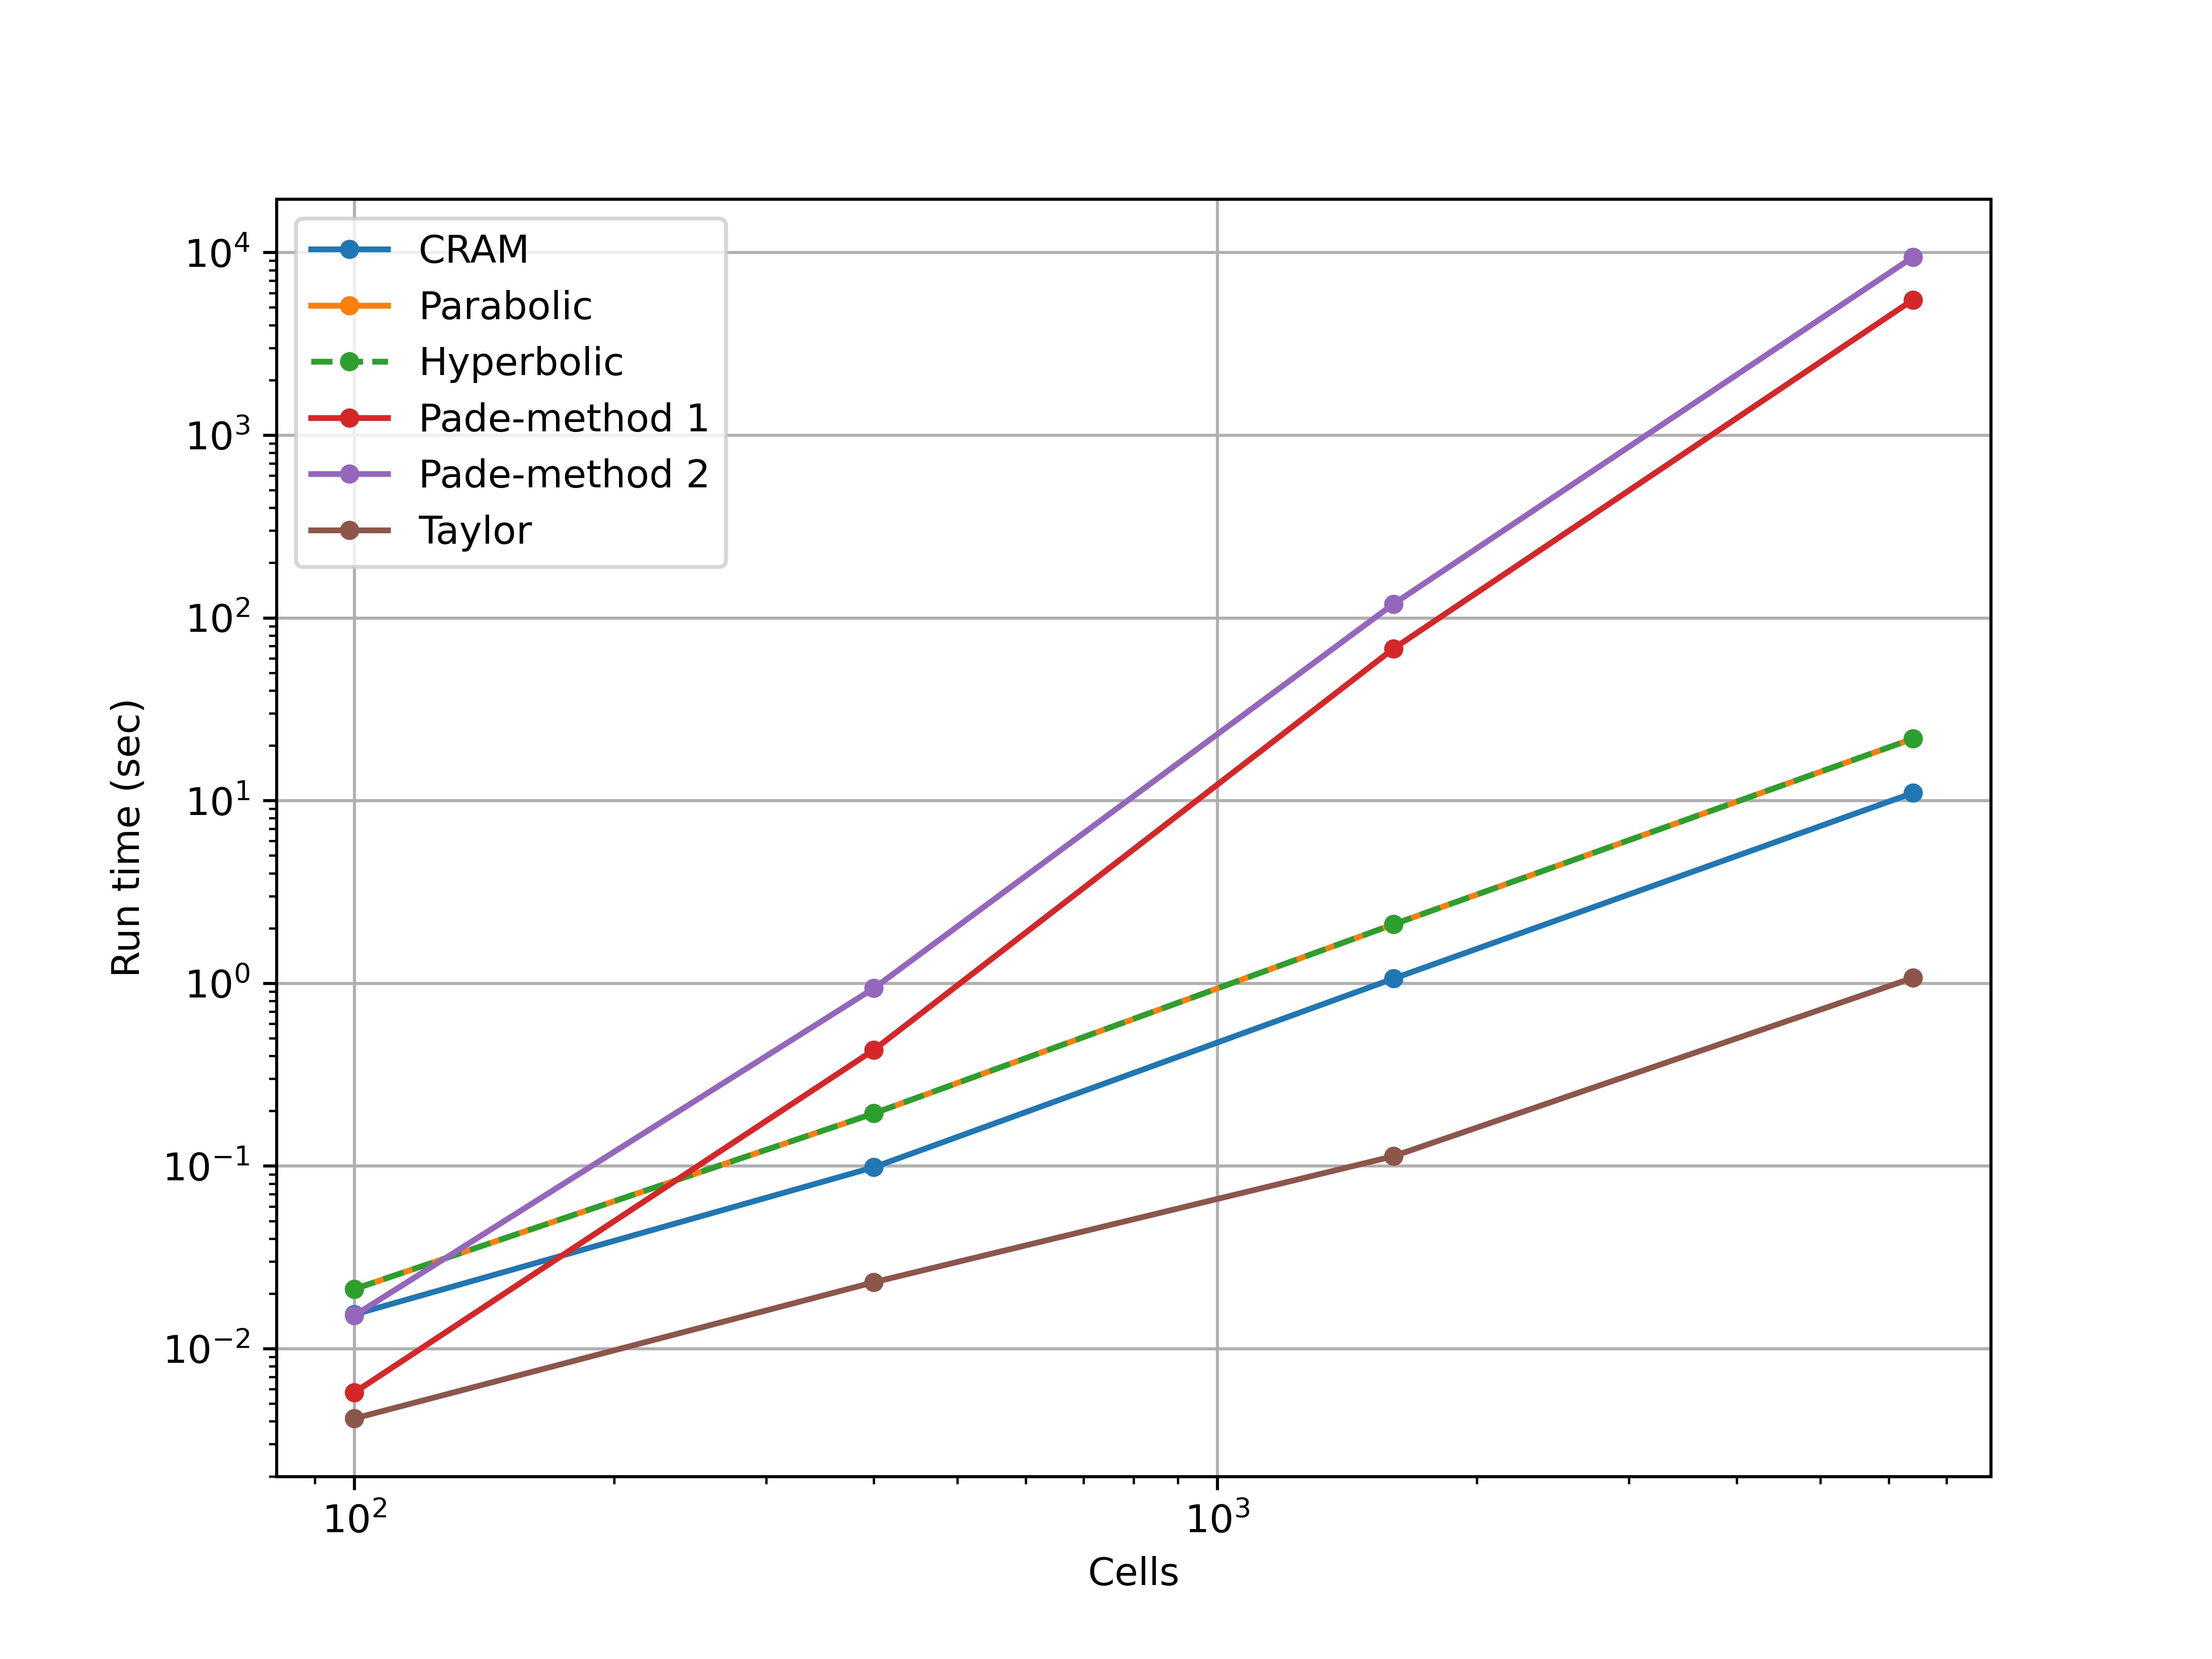
\includegraphics[width=5in]{images/chapter-5/progressionProblems/problem1/diffusionProblem1Runtime.png}
    \caption{Run time performance for diffusion problem one}
    \label{fig:runtime_diffusion_one}
\end{figure}

\clearpage

\begin{figure}[p]
    \centering
    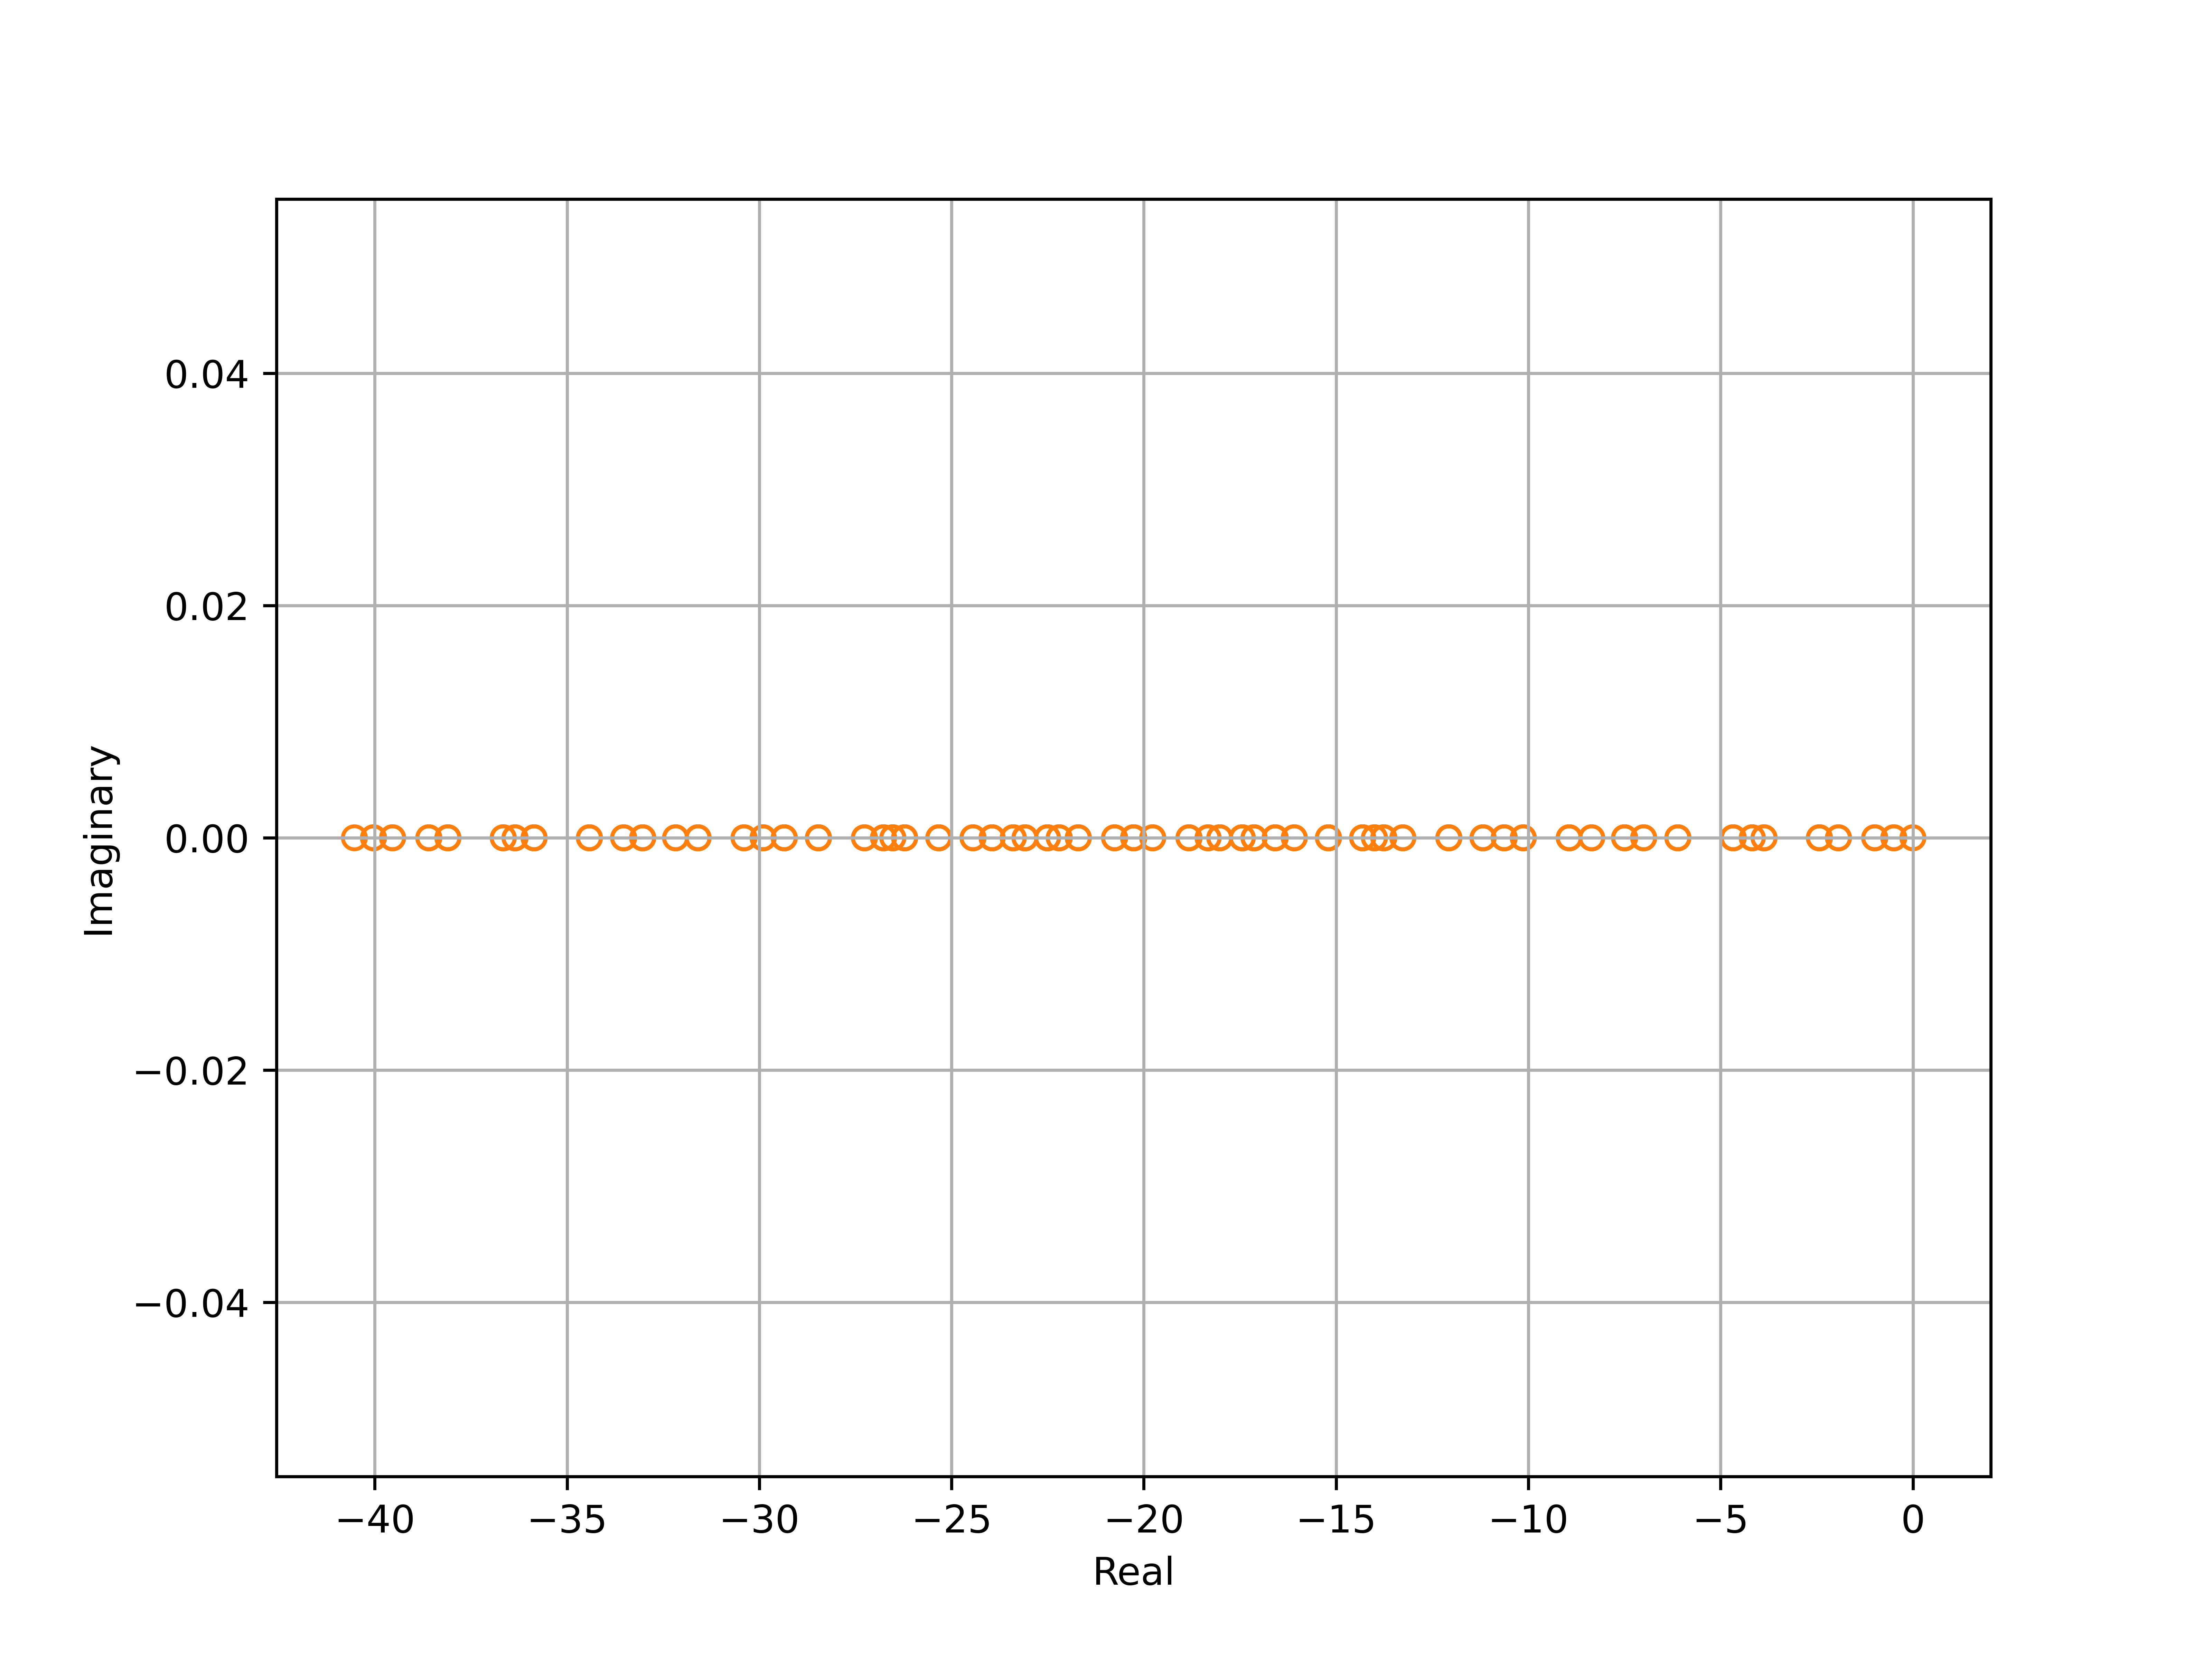
\includegraphics[width=5in]{images/chapter-5/progressionProblems/problem1/eigenvaluesDiffusion1-20.png}
    \caption{Eigenvalues for the 400 x 400 case in diffusion problem one}
    \label{fig:eigenvalues_diffusion_one}
\end{figure}

\clearpage

\begin{table}[p]
   \caption{\label{tab:diffusion_problem1_results_krylov} Error and Run Times for Different Krylov Subspace Dimensions}
   \centering
   \begin{tabular}{cllllll}
   \hline
   Solver & M & $l_{\infty}$ Error & $l_{1}$ Error & $l_{2}$ Error & Run time (sec)\\
   \hline
   Pad\'e-method 1 &   5 & 1.74e-05 & 7.05e-06 & 1.12e-02 & 1.13e-02 \\
   - &  10 & 1.74e-05 & 7.05e-06 & 1.12e-02 & 1.47e-02 \\
   - &  25 & 1.74e-05 & 7.05e-06 & 1.12e-02 & 3.31e-02 \\
   - &  50 & 1.74e-05 & 7.05e-06 & 1.12e-02 & 9.27e-02 \\
   - & 100 & 1.74e-05 & 7.05e-06 & 1.12e-02 & 3.33e-01 \\
   - & 150 & 1.74e-05 & 7.05e-06 & 1.12e-02 & 7.30e-01 \\
   - & 200 & 1.74e-05 & 7.05e-06 & 1.12e-02 & 1.33e+00 \\
   \hline
   Pad\'e-method 2 &   5 & 1.74e-05 & 7.05e-06 & 1.12e-02 & 9.15e-03 \\
   - &  10 & 1.74e-05 & 7.05e-06 & 1.12e-02 & 1.18e-02 \\
   - &  25 & 1.74e-05 & 7.05e-06 & 1.12e-02 & 2.96e-02 \\
   - &  50 & 1.74e-05 & 7.05e-06 & 1.12e-02 & 8.95e-02 \\
   - & 100 & 1.74e-05 & 7.05e-06 & 1.12e-02 & 3.28e-01 \\
   - & 150 & 1.74e-05 & 7.05e-06 & 1.12e-02 & 8.20e-01 \\
   - & 200 & 1.74e-05 & 7.05e-06 & 1.12e-02 & 1.55e+00 \\
   \hline
   \end{tabular}
\end{table}


\FloatBarrier
\clearpage

\subsection{Problem 2}
In the second example, a 1D reaction-diffusion problem was modeled. This problem was taken from work performed by Chou et al. (\cite{ching2007}). The partial differential equations (PDEs) are as follows:

\begin{equation}
\setlength{\jot}{15pt}
\begin{split}
    \frac{\partial U}{\partial t} &= d\frac{\partial^{2}U}{\partial x^{2}} - aU + V, \\
    \frac{\partial V}{\partial t} &=
    d\frac{\partial^{2}V}{\partial x^{2}} - bV,
\end{split}
    \label{eq:problem2Eqs}
\end{equation}

\noindent on the domain $x \in [0, \pi/2]$. The system is subject to the following boundary conditions: 

\begin{equation}
    \frac{\partial U}{\partial x}(0,t) = 0, \quad \frac{\partial V}{\partial x}(0,t) = 0, \quad U(\frac{\pi}{2}, t) = 0, \quad V(\frac{\pi}{2}, t)= 0,
\end{equation}

\noindent with the following initial condition:

\begin{equation}
    U(x,0) = 2\cos(x), \quad V(x,0) = (a-b)\cos(x).
\end{equation}

\noindent The exact solution is given by

\begin{equation}
\setlength{\jot}{15pt}
\begin{split}
    U(x,t) = \bigg( e^{-(a+d)t} + e^{-(b+d)t}\bigg)\cos(x), \text{ and} \\
    V(x,t) = (a - b) e^{-(b+d)t}\cos(x).
\end{split}
\end{equation}

The same three test problems that were conducted in the work by Chou et al. (\cite{ching2007}) were also conducted in libowski. These test results correspond to changes in coefficients $[a, b, d]$, which produced a diffusion-dominated system [0.1, 0.01, 1.0], a reaction-dominated system [2.0, 1.0, 0.001], and a stiff reaction system [100, 1.0, 0.001]. Each test case was run with one time step to $t = 1$, so $\Delta t = 1$. The number of cells in the x direction was varied from 10 to 320. Results for the spatial convergence for the Taylor solver for the diffusion-dominated, reaction-dominated and stiff reaction--dominated cases are shown in Tables \ref{tab:diffusion_spatial_convergence_diffusion_dom}, \ref{tab:diffusion_spatial_convergence_reaction_dom}, and \ref{tab:diffusion_spatial_convergence_stiff_reaction_dom}. Each solver produced the same error at up to four decimal places for most of the $n$ values; therefore, only the Taylor results are shown. Full results for these test are shown in Appendix \ref{appen:results} Tables \ref{tab:diffusion_diffusion_dom_problem2_results}, \ref{tab:diffusion_reaction_dom_problem2_results} and \ref{tab:diffusion_stiff_reaction_dom_problem2_results}. As expected, the convergence rate for this problem is second order or better for each of the error metrics.  While there is little difference between the errors from these solvers for this first problem, there is a notable difference in run times for the Pad\'e and Taylor solvers. The E${}_{\infty}$ error and run time for each sub-problem is shown in Figures \ref{fig:problem2_diffusion_dom}, \ref{fig:problem2_reaction_dom} and \ref{fig:problem2_stiff_reaction_dom}. 

Figures \ref{fig:problem2_diffusion_dom}-\ref{fig:problem2_stiff_reaction_dom} show that CRAM is the fastest solver, followed by the parabolic and hyperbolic solvers. Both of the Pad\'e solvers had drastically much longer run times for the diffusion-dominated cases, with Method 2 being the longest. Interestingly, the Taylor solver showed dramatically different run times based on the physical process dominating the problem. In the diffusion-dominated cases, the Taylor solver took the longest, but in the reaction-dominated cases, the run time was on the order of the CRAM, parabolic, and hyperbolic solvers. 

The Krylov subspace approximation was applied to each sub-problem with 1,000 cells in the x direction. The Krylov dimensions were varied from 2 to 100, and the results are shown in Figure \ref{fig:problem2_krylov} . Unlike the previous diffusion example, a much larger Krylov dimension was required to reach a converged error in the diffusion-dominated case. Each solver showed the same error behavior, but with slightly different converged errors due to numerical accuracy in the algorithms. Each solver also showed similar behavior, with run time scaling as a function of the Krylov dimension; however, each axis was scaled differently. Applying the Krylov subspace to each Pad\'e solver reduced the many orders of magnitude, but it failed to reduce the run time of the Taylor solver to the same order in the diffusion-dominated case. For each of the reaction-dominated cases, the Krylov subspace dimension required to reach a converged solution is much smaller than the diffuion-dominated case. 

\clearpage

\begin{table}[h]
   \caption{\label{tab:diffusion_spatial_convergence_diffusion_dom} Convergence Rate for Diffusion-Dominated Problem Using Absolute Error}
   \centering
   \begin{tabular}{lllllll}
   \hline
    n & E${}_{\infty}$ Rate & E${}_{1}$ Rate & E${}_{2}$ Rate & E${}_{\infty}$ Error & E${}_{1}$ Error & E${}_{2}$ Error\\
   \hline
    20 & 2.00 & 2.00 & 2.50 & 1.87e-04 & 1.19e-04 & 2.97e-05 \\ 
    40 & 2.00 & 2.00 & 2.50 & 4.69e-05 & 2.99e-05 & 5.24e-06 \\ 
    80 & 2.00 & 2.00 & 2.50 & 1.17e-05 & 7.46e-06 & 9.27e-07 \\ 
   160 & 2.00 & 2.00 & 2.50 & 2.93e-06 & 1.87e-06 & 1.64e-07 \\ 
   320 & 2.00 & 2.00 & 2.50 & 7.33e-07 & 4.66e-07 & 2.90e-08 \\ 
   \hline
   \end{tabular}
\end{table}

\begin{table}[h]
   \caption{\label{tab:diffusion_spatial_convergence_reaction_dom} Convergence Rate for Reaction-Dominated Problem Using Absolute Error}
   \centering
   \begin{tabular}{lllllll}
   \hline
    n & E${}_{\infty}$ Rate & E${}_{1}$ Rate & E${}_{2}$ Rate & E${}_{\infty}$ Error & E${}_{1}$ Error & E${}_{2}$ Error\\
   \hline
    20 & 2.00 & 2.00 & 2.50 & 2.23e-04 & 1.42e-04 & 3.53e-05 \\  
    40 & 2.00 & 2.00 & 2.50 & 5.58e-05 & 3.55e-05 & 6.24e-06 \\  
    80 & 2.00 & 2.00 & 2.50 & 1.40e-05 & 8.88e-06 & 1.10e-06 \\  
   160 & 2.00 & 2.00 & 2.50 & 3.49e-06 & 2.22e-06 & 1.95e-07 \\  
   320 & 2.00 & 2.00 & 2.50 & 8.72e-07 & 5.55e-07 & 3.45e-08 \\  
   \hline
   \end{tabular}
\end{table}

\begin{table}[h]
   \caption{\label{tab:diffusion_spatial_convergence_stiff_reaction_dom} Convergence Rate for Stiff Reaction--Dominated Problem Using Absolute Error}
   \centering
   \begin{tabular}{lllllll}
   \hline
    n & E${}_{\infty}$ Rate & E${}_{1}$ Rate & E${}_{2}$ Rate & E${}_{\infty}$ Error & E${}_{1}$ Error & E${}_{2}$ Error\\
   \hline
    20 & 2.00 & 2.00 & 2.50 & 9.42e-03 & 6.00e-03 & 1.49e-03 \\ 
    40 & 2.00 & 2.00 & 2.50 & 2.36e-03 & 1.50e-03 & 2.63e-04 \\ 
    80 & 2.00 & 2.00 & 2.50 & 5.89e-04 & 3.75e-04 & 4.66e-05 \\ 
   160 & 2.00 & 2.00 & 2.50 & 1.47e-04 & 9.38e-05 & 8.23e-06 \\ 
   320 & 2.00 & 2.00 & 2.50 & 3.68e-05 & 2.34e-05 & 1.46e-06 \\ 
   \hline
   \end{tabular}
\end{table}

\clearpage

\begin{figure}[p]
    \centering
    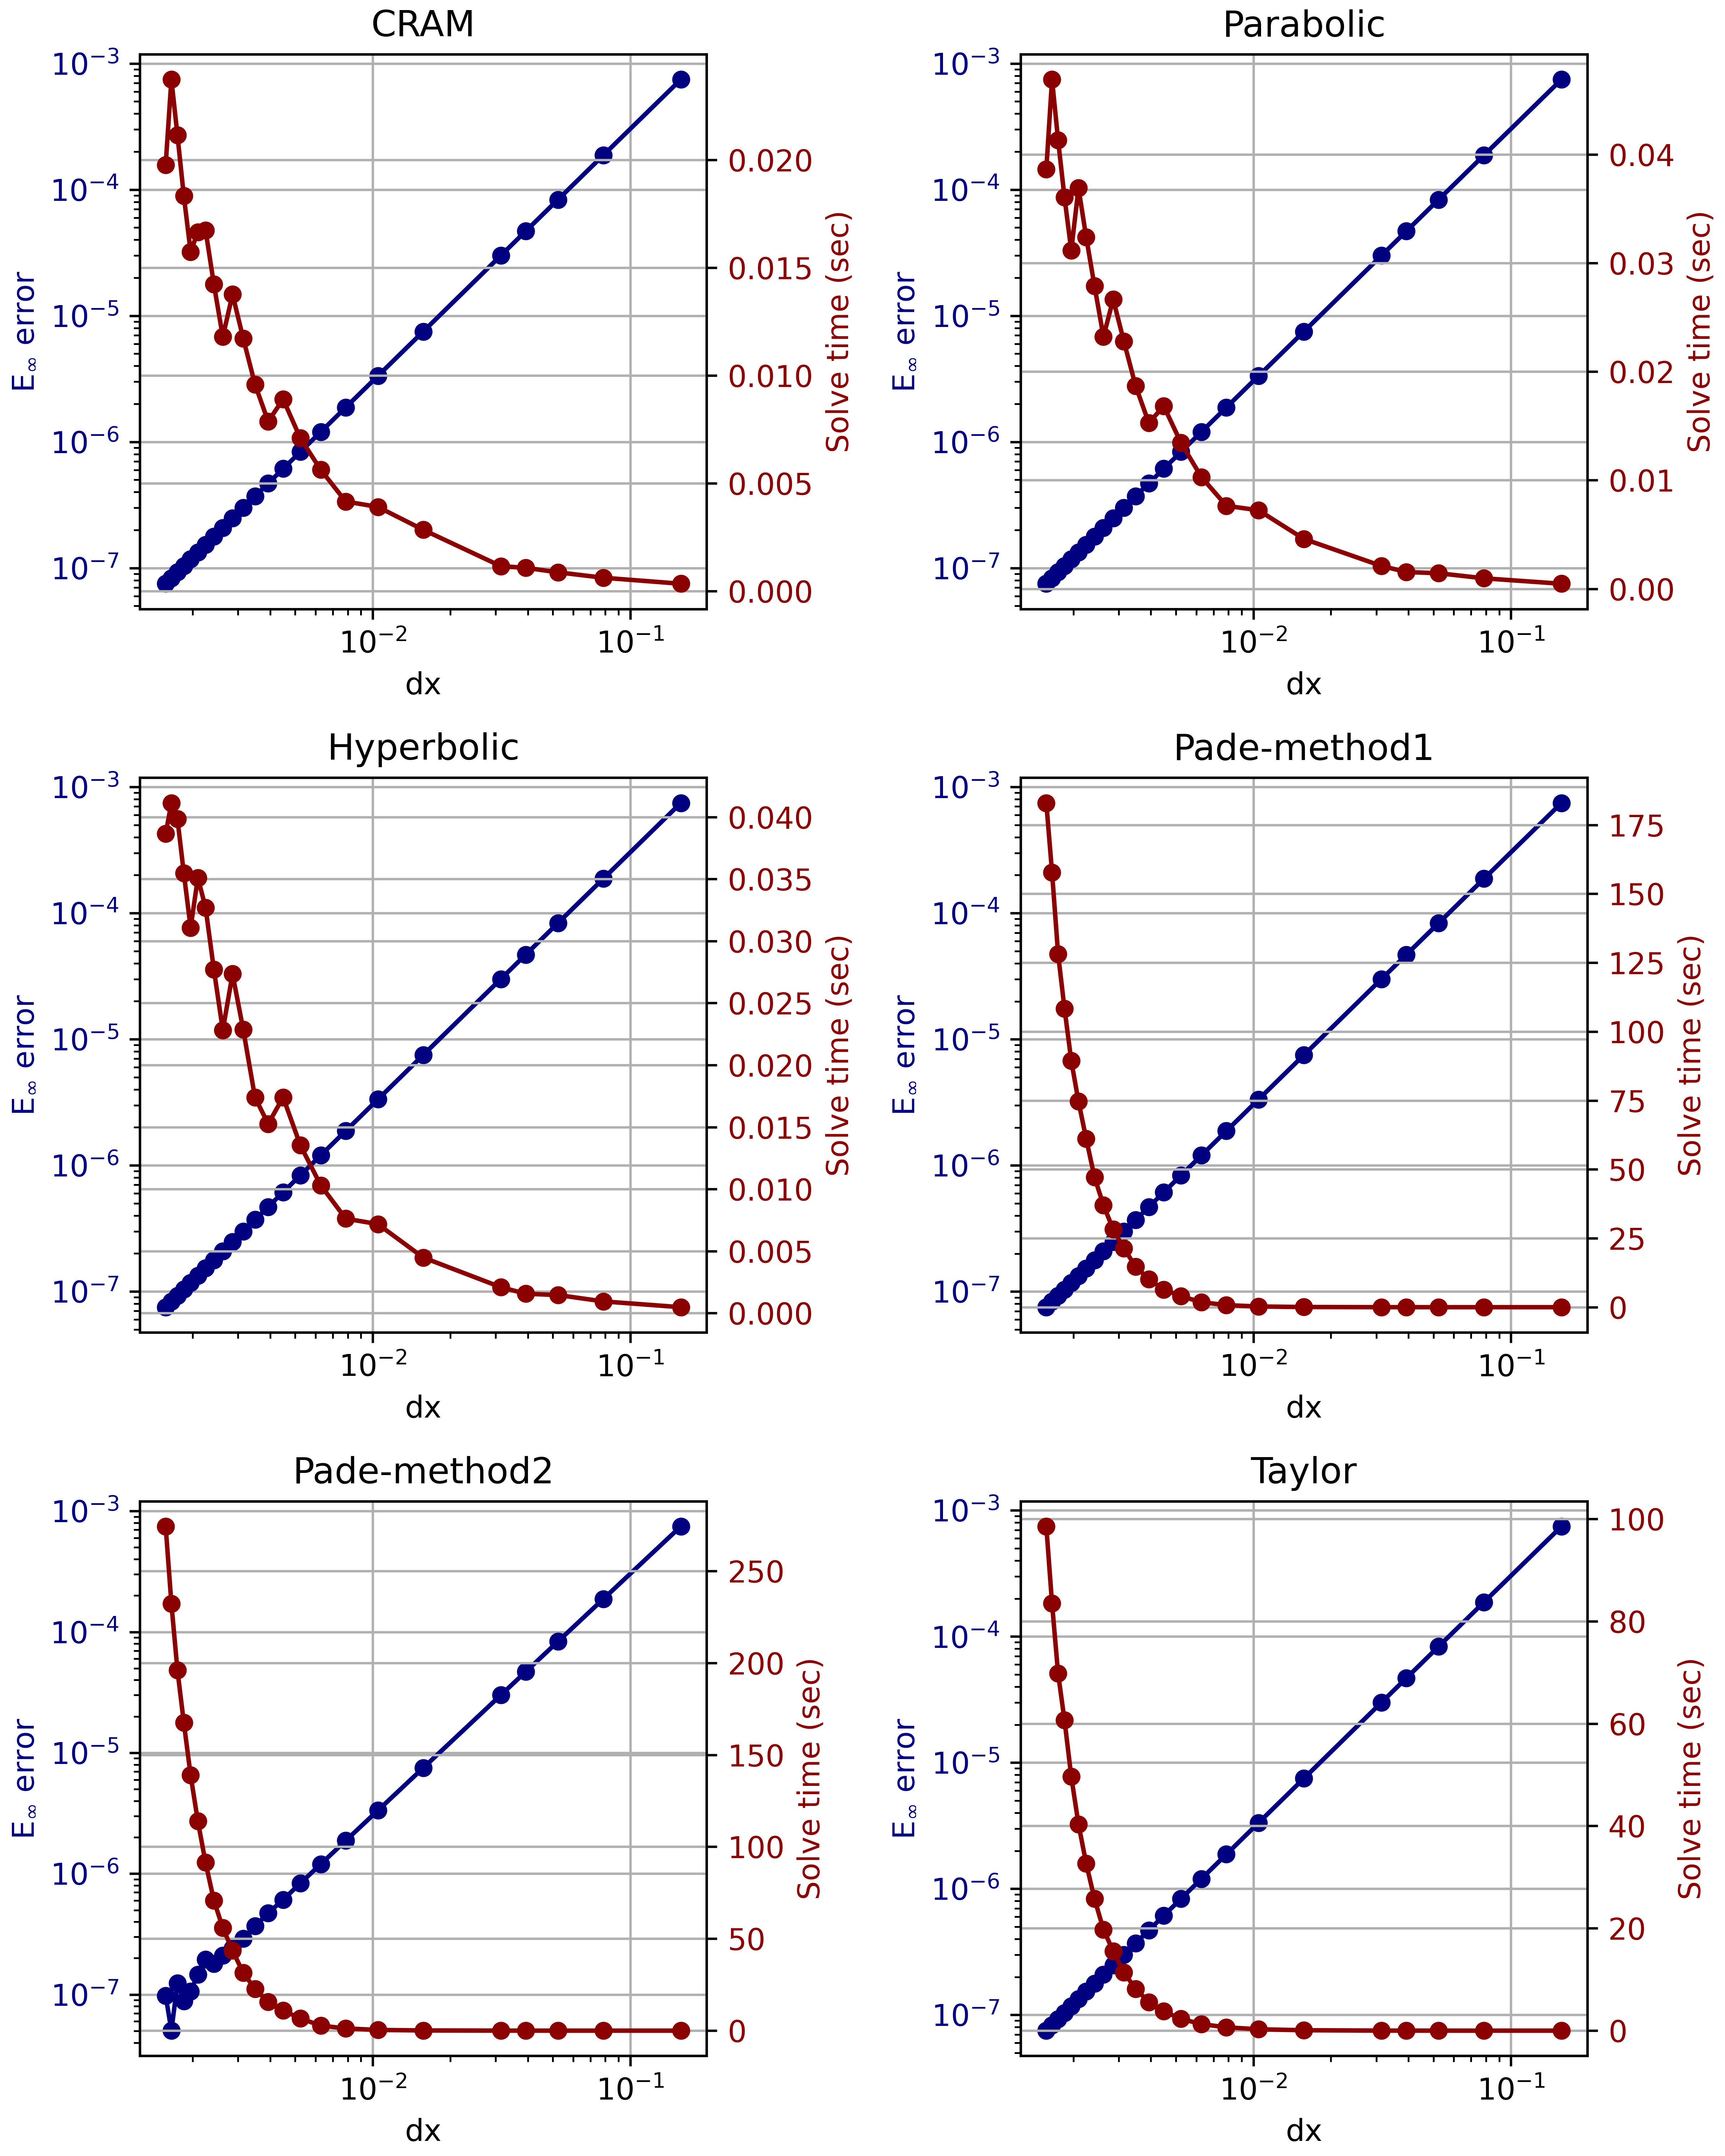
\includegraphics[width=5.0in]{images/chapter-5/progressionProblems/problem2/problem2a.png}
    \caption{Results for the diffusion-dominated case}
    \label{fig:problem2_diffusion_dom}
\end{figure}

\clearpage

\begin{figure}[p]
    \centering
    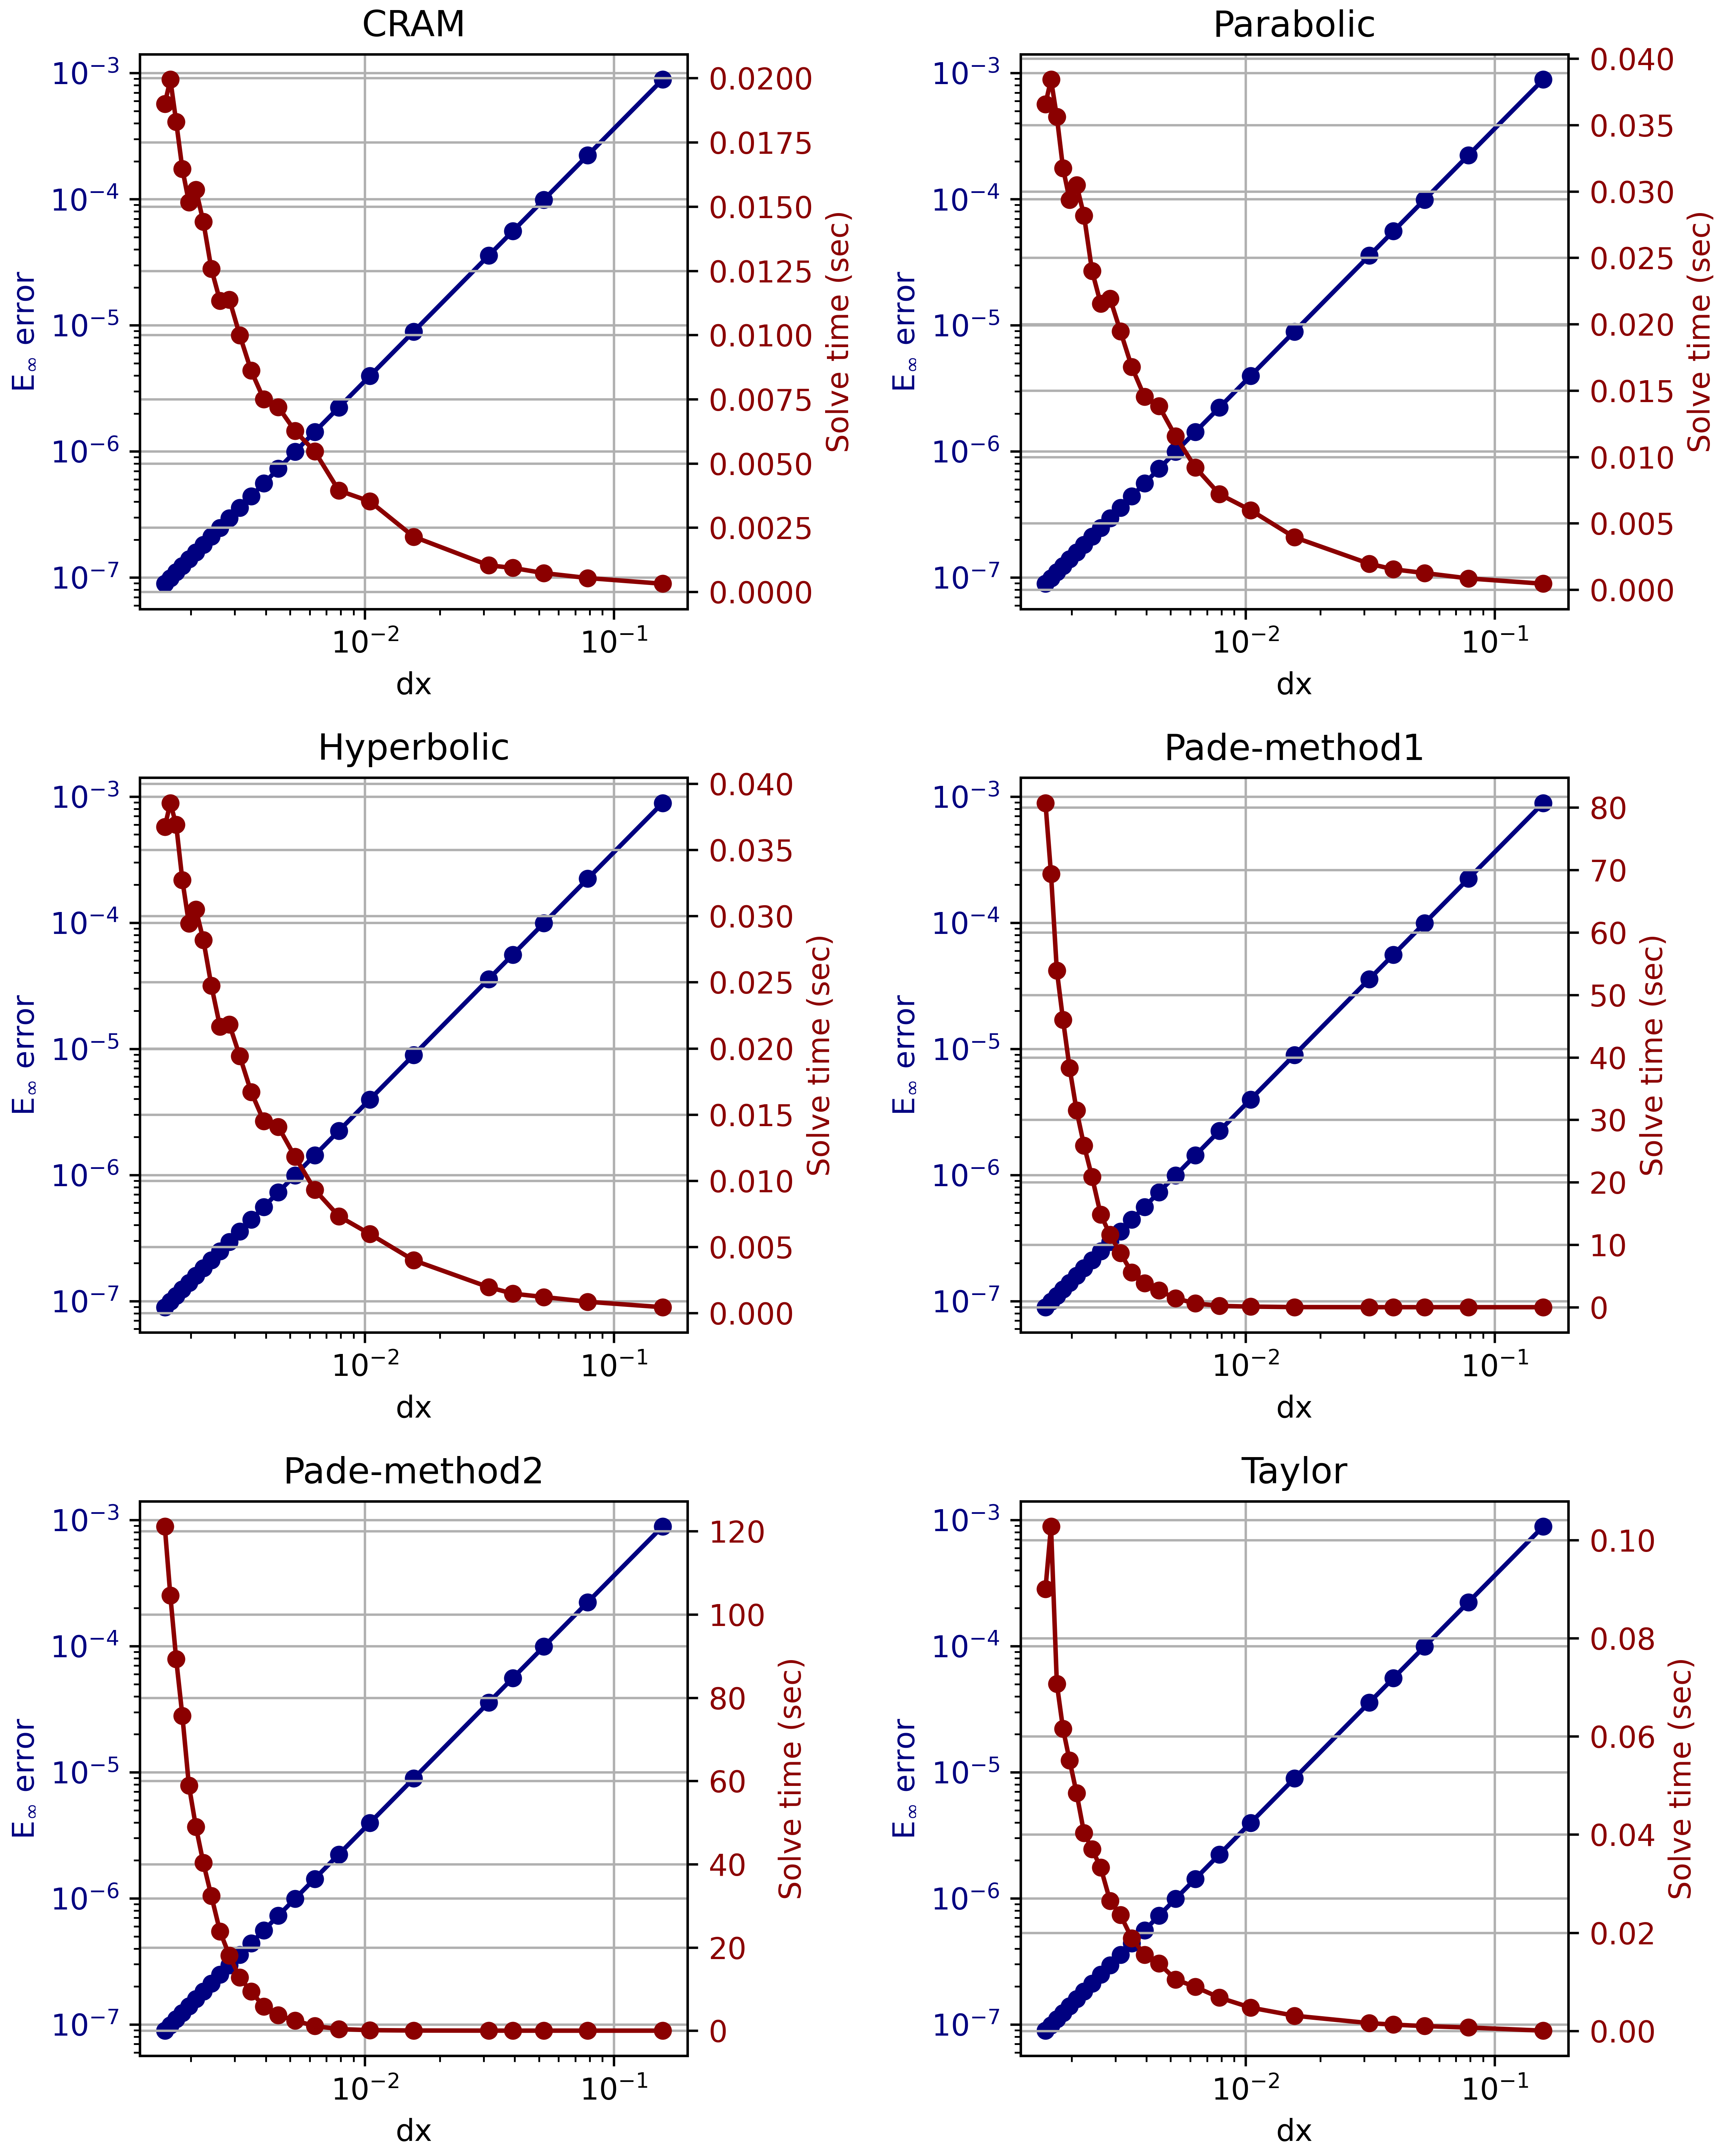
\includegraphics[width=5.0in]{images/chapter-5/progressionProblems/problem2/problem2b.png}
    \caption{Results for the reaction-dominated case}
    \label{fig:problem2_reaction_dom}
\end{figure}

\clearpage

\begin{figure}[p]
    \centering
    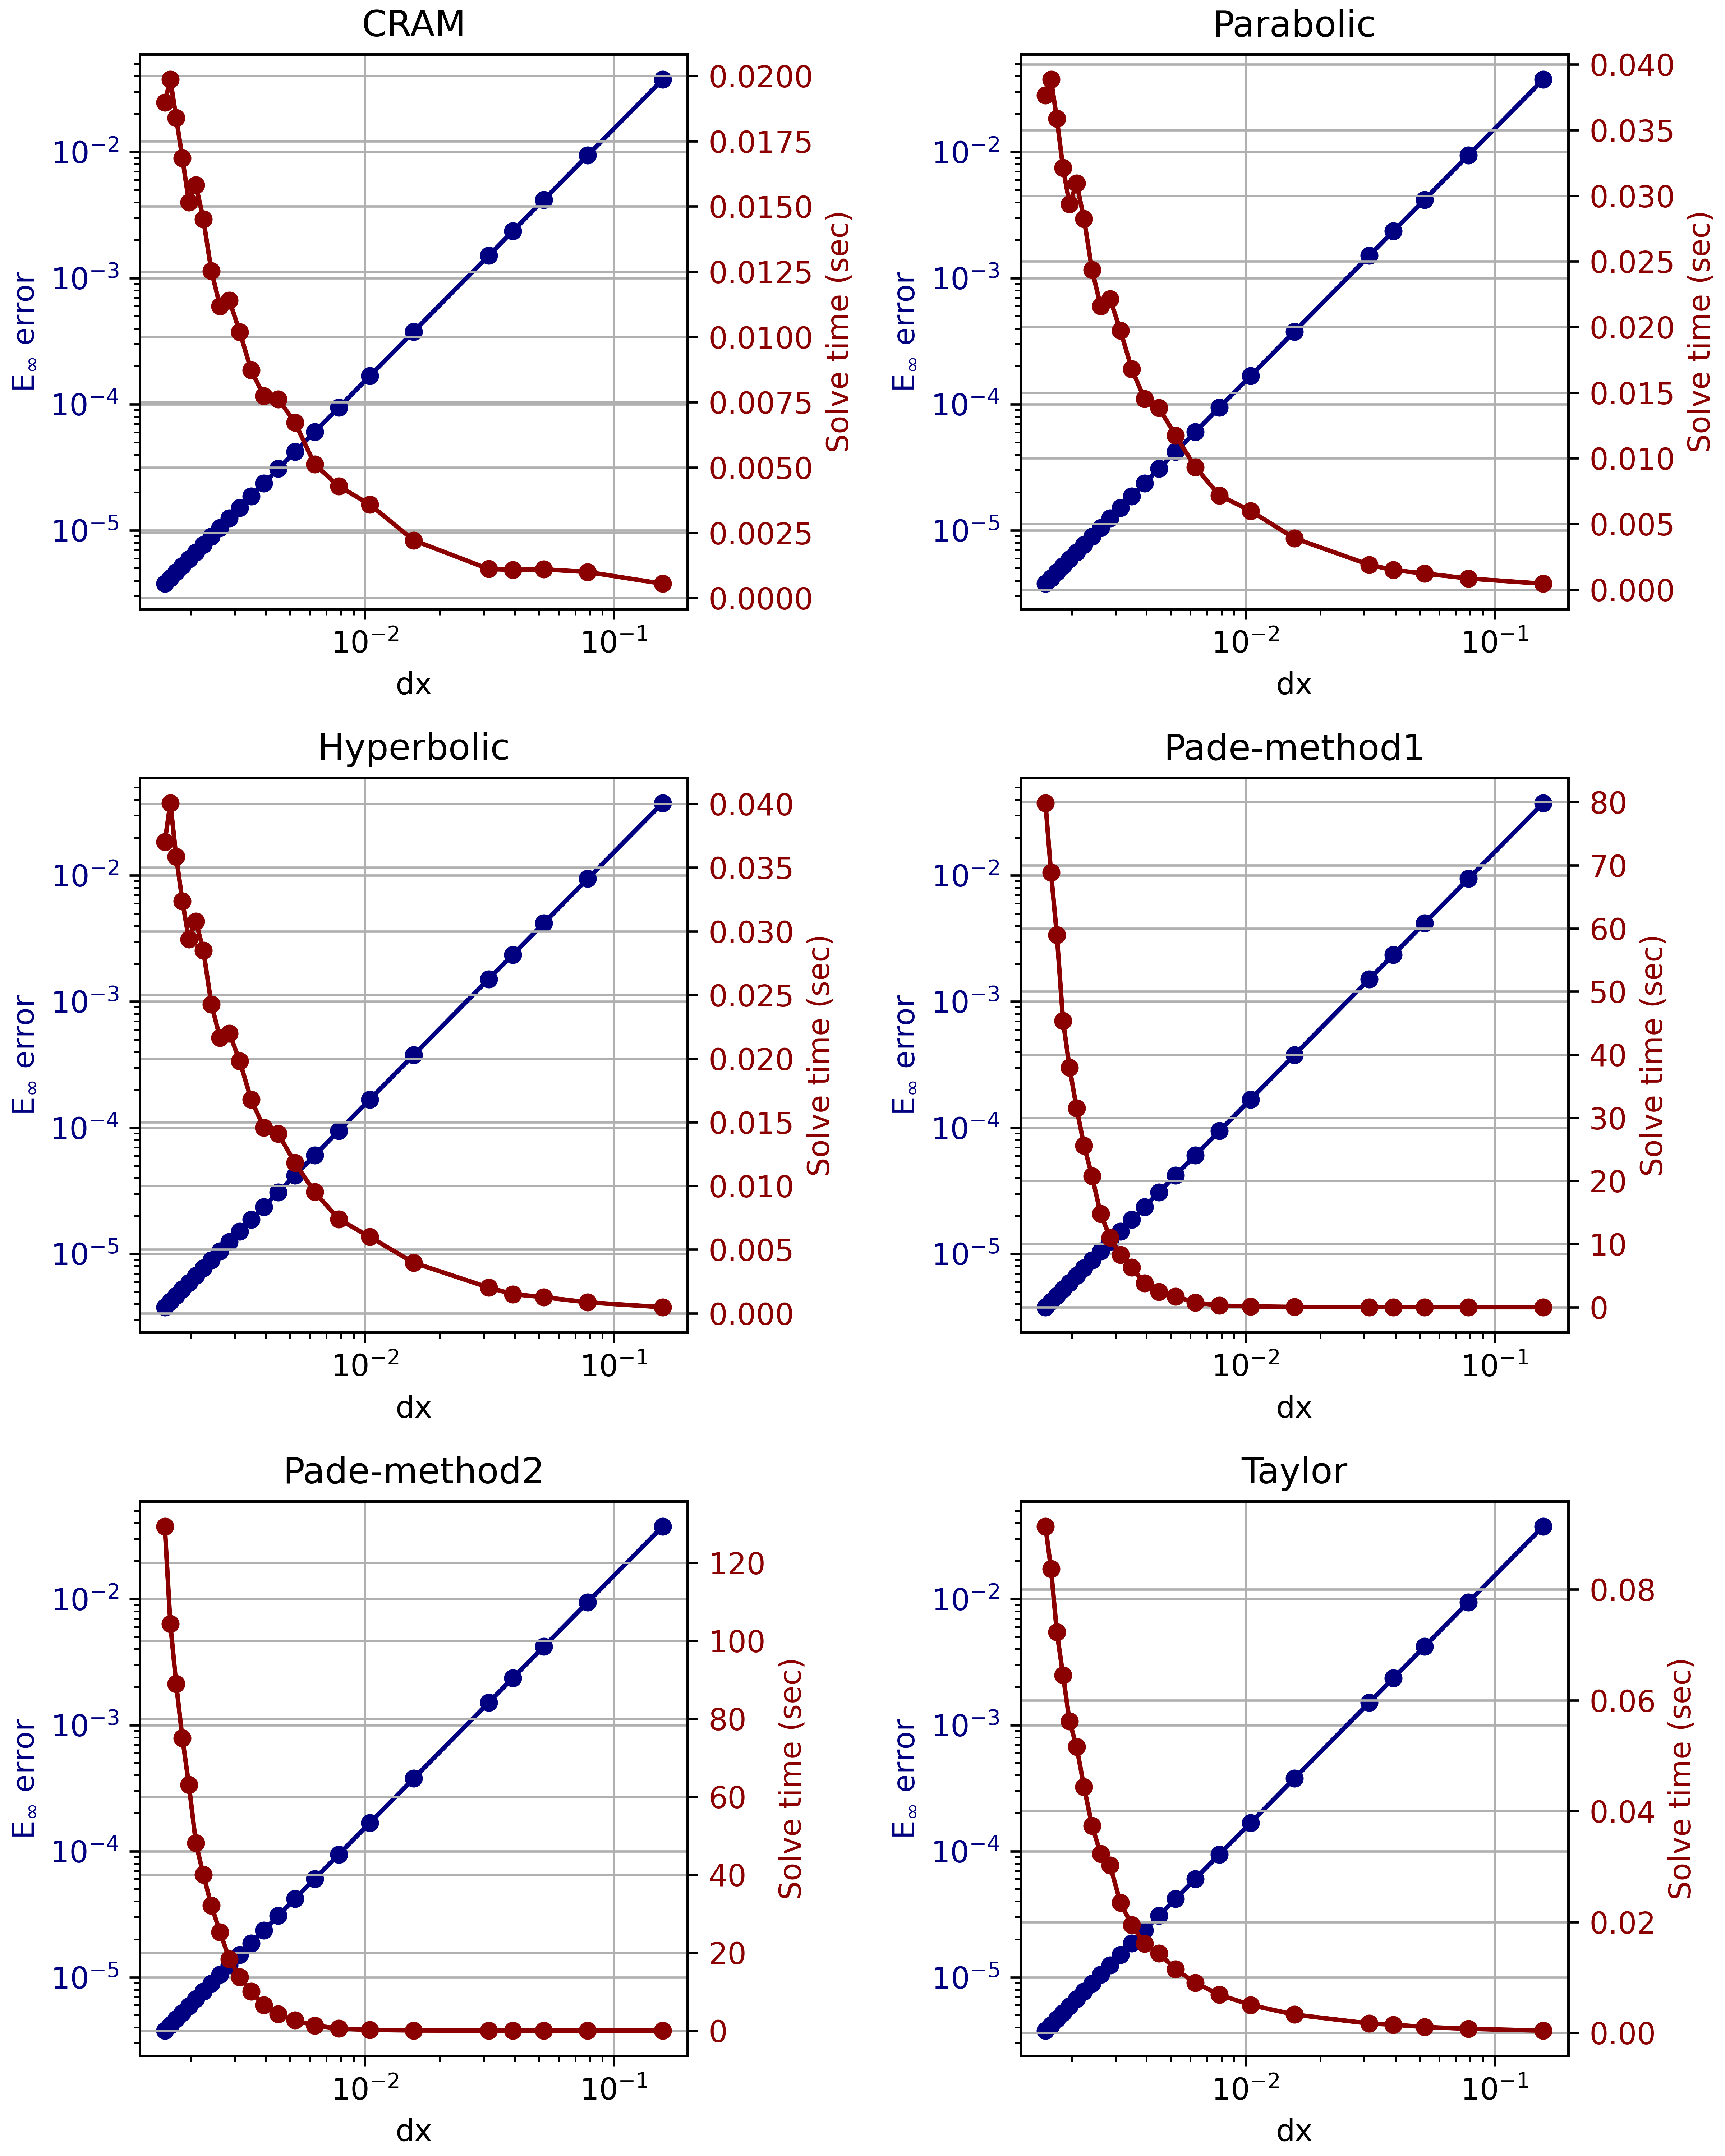
\includegraphics[width=5.0in]{images/chapter-5/progressionProblems/problem2/problem2c.png}
    \caption{Results for the stiff reaction-dominated case}
    \label{fig:problem2_stiff_reaction_dom}
\end{figure}

\clearpage

\begin{landscape}
\thispagestyle{mylandscape}
\begin{figure}[p]
    \centering
    \includegraphics[width=8in]{images/chapter-5/progressionProblems/problem2/krylovProblem2.png}
    \caption{Results for the Krylov subspace approximation for each sub-problem}
    \label{fig:problem2_krylov}
\end{figure}
\end{landscape}

\clearpage

\subsection{Problem 3}

Convection was tested using PDE of the form

\begin{equation}
    \frac{\partial U}{\partial t} = -v\frac{\partial U}{\partial x},
    \label{eq:convection_PDE}
\end{equation}

\noindent where $v$ is velocity. Equation (\ref{eq:convection_PDE}) was applied to a system on the domain $x \in [0, 100]$, $t \in [0, 20]$ subject to the following boundary conditions:

\begin{equation}
    U(0,t) = 1.0, \quad\frac{\partial U}{\partial x}(100, t) = 0.0,
\end{equation}

\noindent and the initial condition:

\begin{equation}
    U(x,0) = 0.0.
\end{equation}

What is most important about this problem is that it exposes an instability with Cauchy solvers which seems to be specific to this problem. This is something that is not seen with the series solvers such as Pad\'e or Taylor. First, results for the first order upwind differencing scheme are shown in Figure \ref{fig:first_order_results}  for a first-order backward differencing formula (BDF1) and the ETD scheme using the series matrix exponential solvers. While only the Taylor solver is shown, results for the Pad\'e solvers are the same. Figure \ref{fig:first_order_results} shows the typical reduction in numerical diffusion with decreasing dx. In Figure \ref{fig:first_order_results} we see that as the time step size decreases for the explicit BDF1 solver it approaches the accuracy of the ETD method with a single time step. 

The instability seen with Cauchy solvers is shown in Figure \ref{fig:first_order_results_cauchy_instability} for a zoomed in and zoomed out view of each solution. In Figure \ref{fig:first_order_results_cauchy_instability} it is seen that for dx values 0.5 and 0.4, the solution blows up and oscillates. What is important to note that even know the solution for dx = 1.0 is stable it does contain small negative values as it approaches zero. The matrix exponential is the analytical solution to the ODE system and should not show any instability, so the instability shown here is due to the numerical computation of the exponential itself. 

\clearpage

\begin{figure}[p]
    \centering
    \includegraphics[width=6in]{images/chapter-5/progressionProblems/problem3/problem3FirstOrder.png}
    \caption{First-order upwind differencing with series solvers and BDF1}
    \label{fig:first_order_results}
\end{figure}

\clearpage

\begin{figure}[p]
    \centering
    \includegraphics[width=6.0in]{images/chapter-5/progressionProblems/problem3/problem3FirstOrderCauchyInstability.png}
    \caption{First-order upwind differencing instability for Cauchy solvers}
    \label{fig:first_order_results_cauchy_instability}
\end{figure}

\clearpage


\noindent To combat this instability the order of the method can be increased, this is seen in Figure \ref{fig:first_order_results_cauchy_instability_different_orders}. Figure \ref{fig:first_order_results_cauchy_instability_different_orders} shows the Hyperbolic and Parabolic solvers at different order of N. As the order in increased, the solution becomes more stable.  Another method to increase the stability of the solution is to compute the solution with multiple steps and not just at the final time step. This is equivalent to using the substep method for the Cauchy solvers. Figure \ref{fig:first_order_results_cauchy_instability_different_time_steps} shows results for each of the Cauchy solver for different time step sizes. Even with large time step sizes the solution becomes stable. 

To illustrate the enhanced accuracy of TVD non-linear flux limiters, the same problem is conducted with a variety of limiter functions. This method works to approximate the convection term to at most second order in the case of smooth solutions and reduce numerical diffusion seen in the first order case. Figure \ref{fig:fluxlimiters_problem3} shows results from each of the flux limiter functions in libowski using the Taylor solver. Each of the flux limiter functions reduces the numerical diffusion, seen in the first order upwind case with superbee being the best. While the TVD scheme is designed to remove unphysical oscillations seen in higher order convection schemes, these oscillations are present because of the explicit implementation. Figure \ref{fig:fluxlimiters_instability_problem3} shows these oscillations for six flux limiter functions. This behavior is only present when large time step sizes are used. For some time integration methods, explicit schemes are known to be unstable if large time step sizes are used. In this case the second order correction being calculated from the previous time step causes the solution to become unstable if large enough time steps are taken. This same behavior is seen in all the ETD matrix exponential solvers. 



\subsection{Problem 4}

The same PDE that was shown in the previous problem is tested again:

\begin{equation}
    \frac{\partial U}{\partial t} = -v\frac{\partial U}{\partial x},
    \label{eq:convection_PDE}
\end{equation}

\noindent on the domain $x \in [0, 100]$, $t \in [0, 5]$ subject to periodic boundary conditions:

\clearpage

\begin{figure}[p]
    \centering
    \includegraphics[width=5.0in]{images/chapter-5/progressionProblems/problem3/problem3FirstOrderCauchyInstabilityDifferentOrders.png}
    \caption{First-order upwind differencing instability for Cauchy solvers at different orders}
    \label{fig:first_order_results_cauchy_instability_different_orders}
\end{figure}

\clearpage

\begin{figure}[p]
    \centering
    \includegraphics[width=6in]{images/chapter-5/progressionProblems/problem3/problem3FirstOrderCauchyInstabilityDifferentTimeSteps.png}
    \caption{First-order upwind differencing instability for Cauchy solvers at different time step sizes}
    \label{fig:first_order_results_cauchy_instability_different_time_steps}
\end{figure}

\clearpage

\begin{figure}[p]
    \centering
    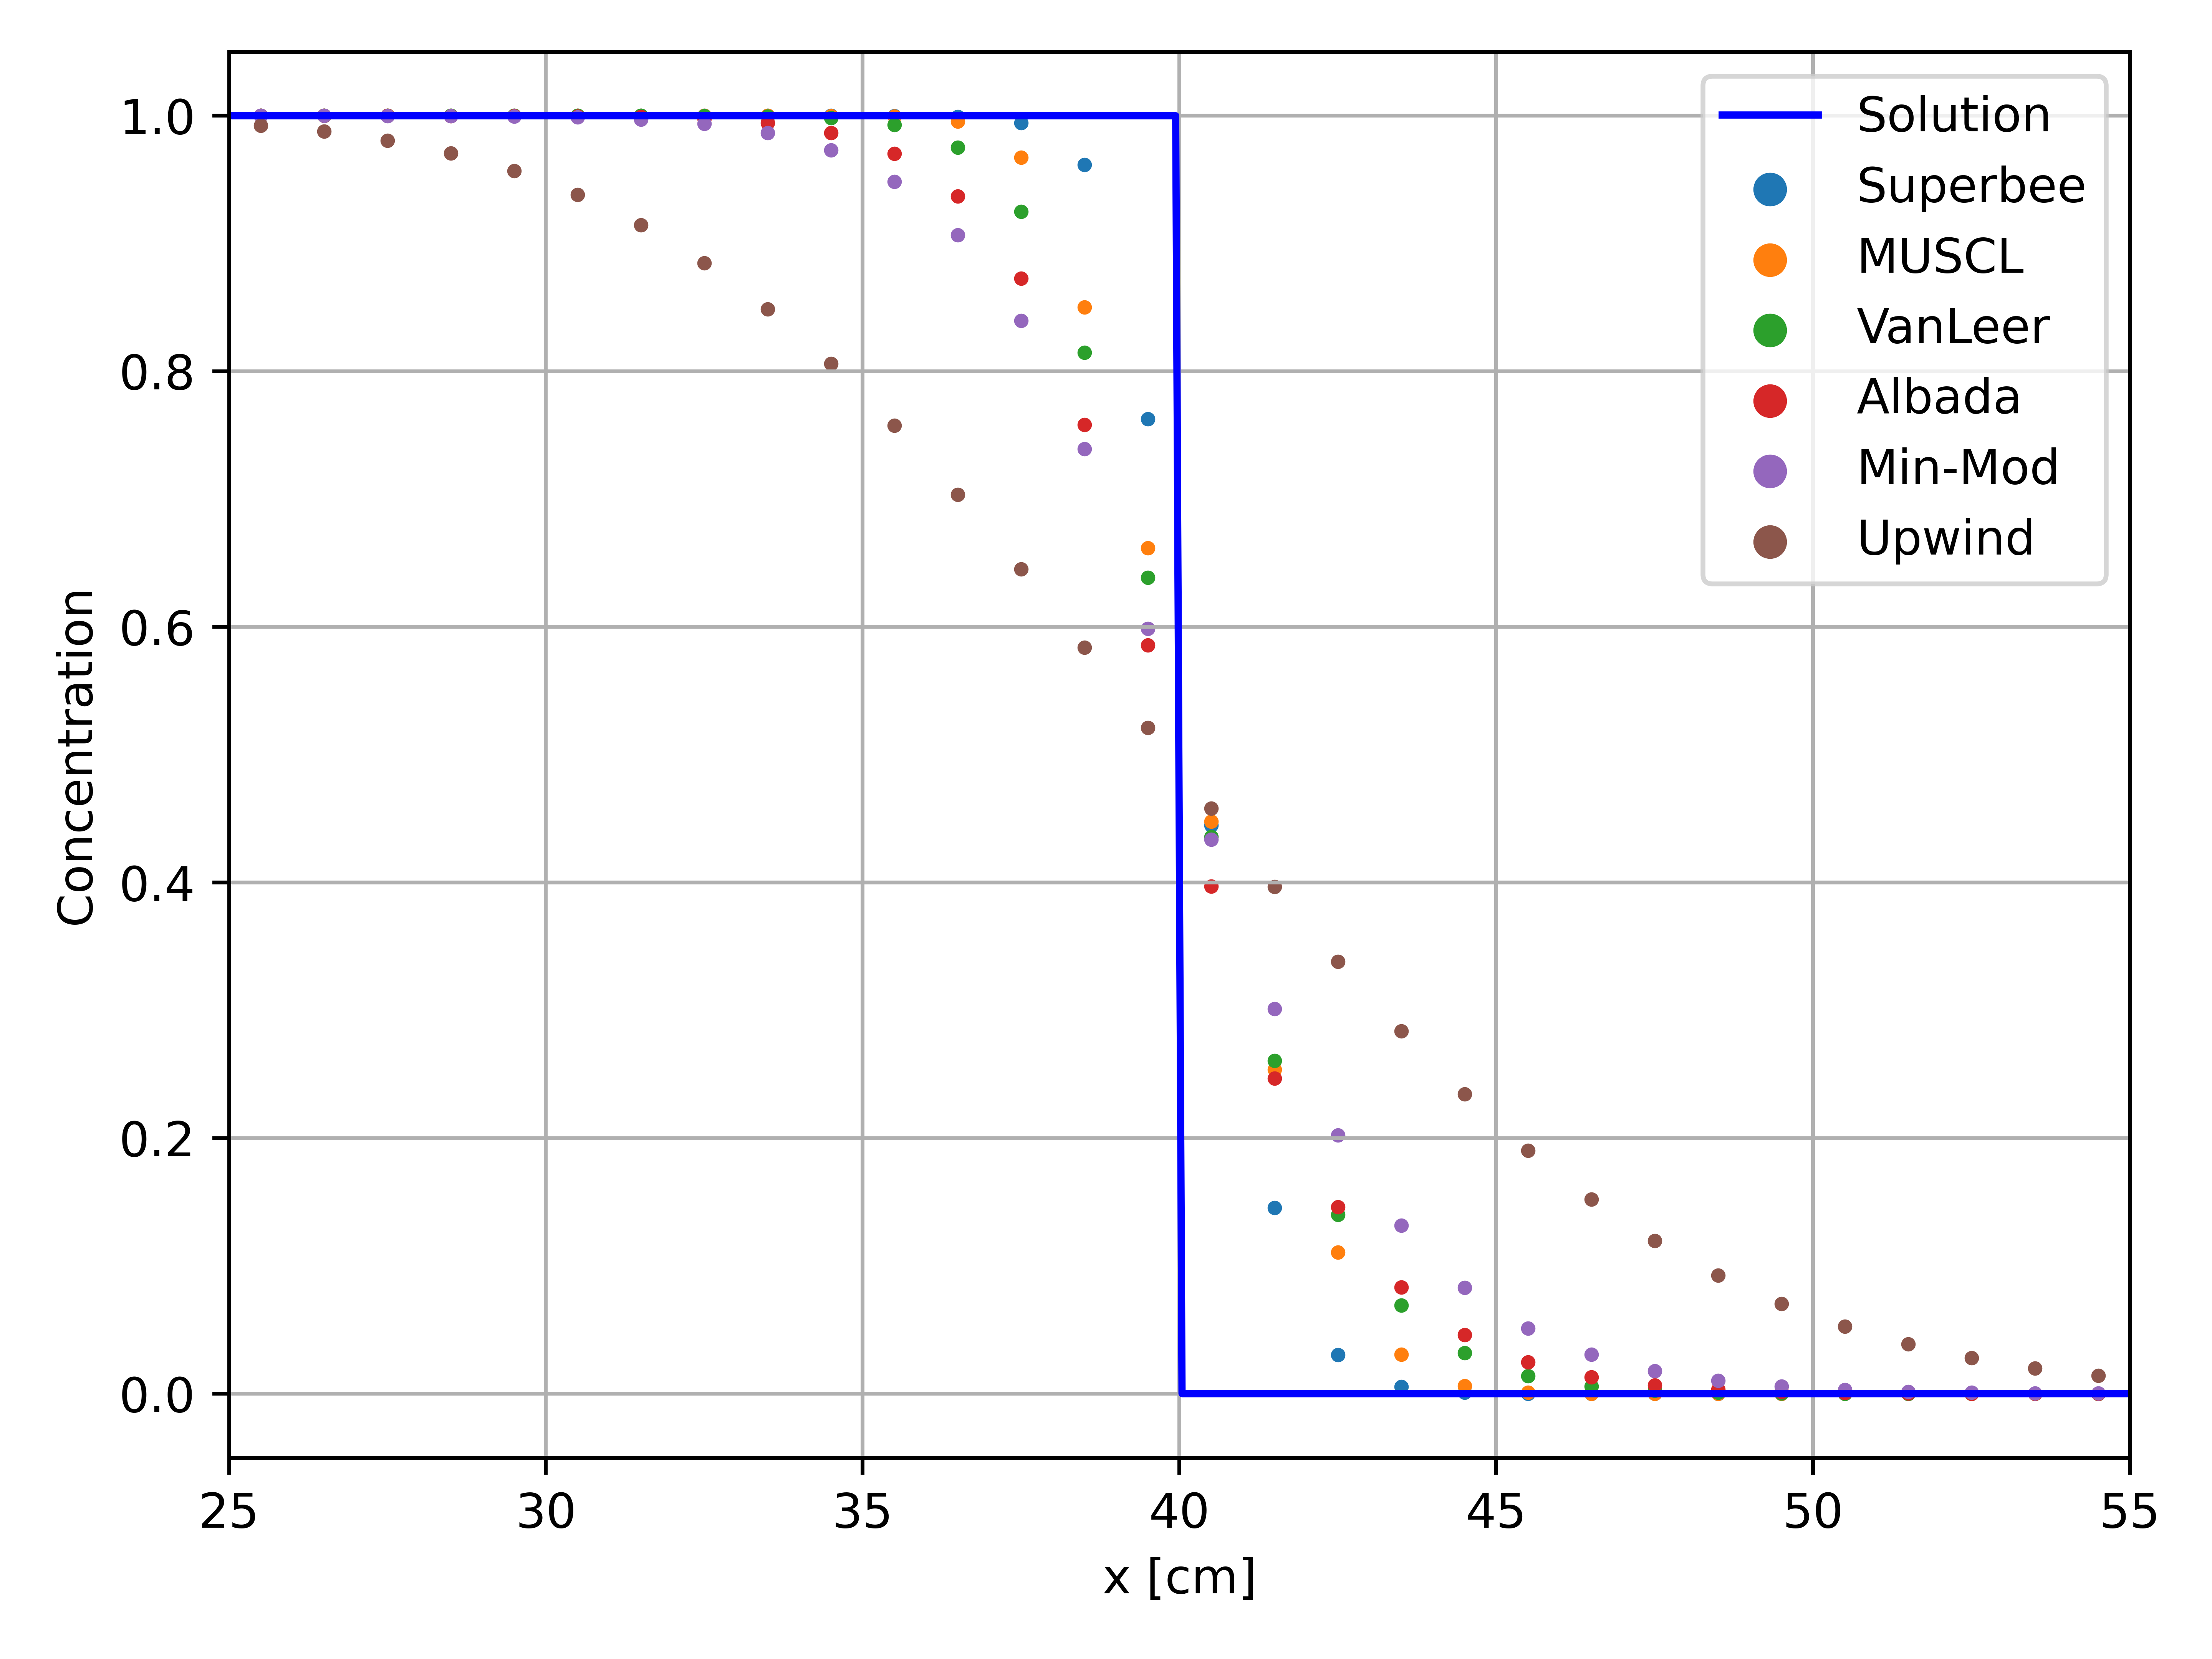
\includegraphics[width=5in]{images/chapter-5/progressionProblems/problem3/problem3FluxLimiters.png}
    \caption{Flux limiter function applied to problem three, dt = 0.1, dx = 0.2}
    \label{fig:fluxlimiters_problem3}
\end{figure}

\clearpage

\begin{figure}[p]
    \centering
    \includegraphics[width=6in]{images/chapter-5/progressionProblems/problem3/problem3SecondOrderFluxLimiterFunctionInstability.png}
    \caption{Instability of flux limiter functions with the Taylor solver}
    \label{fig:fluxlimiters_instability_problem3}
\end{figure}

\clearpage

\begin{equation}
    U(0,t) = U(100, t),
\end{equation}

\noindent and the initial condition:

\begin{equation}
    U(x,0) = \exp\bigg\{-\bigg(\frac{(x-30)}{10}\bigg)^{2}\bigg\}.
\end{equation}

\noindent with the following solution:

\begin{equation}
	U(x,t)_ = \exp\bigg\{-\bigg(\frac{(x-vt-30)}{10}\bigg)^{2}\bigg\}.
\end{equation}

Figure \ref{fig:problem4_l1error_spatial_results} shows E${}_{1}$ error behavior as a function of spatial discretization at various time step sizes. Figure \ref{fig:problem4_l1error_time_results} shows the same error behavior as a function of temporal discretization at various number of spatial cells. Figure \ref{fig:problem4_l1error_spatial_results} shows that as the number of time steps take is increased the higher order flux limiters begin to show a linear relationship with spatial discretization. This can be readily seen with the number of steps greater than 40. The upwind limiter is unaffected by decreasing the time step size, which is to be expected. This is because increasing the number of times steps do nothing to increase its accuracy. Figure \ref{fig:problem4_l1error_time_results} shows that increasing the number of time steps has little to no affect on the error for large spatial discretization. As the number of cells increases, decreasing the time step size has a greater affect on reducing the error. This Figure also reiterates the fact that the first order upwind error is not affected by increasing the number of time steps taken. Results for the E${}_{\infty}$ and E${}_{2}$ errors are shown in Appendix \ref{appen:results} Figures \ref{fig:problem4_linferror_spatial_results}, \ref{fig:problem4_linferror_time_results}, \ref{fig:problem4_l2error_spatial_results} and \ref{fig:problem4_l2error_time_results}. Figure \ref{fig:problem4_linferror_spatial_results} shows a similar trend with spatial refinement using the E${}_{\infty}$ error to the E${}_{1}$ error however, the error function in Figure \ref{fig:problem4_linferror_spatial_results} does not maintain the same linear rate. This relation is further represented in Figure \ref{fig:problem4_linferror_time_results} which shows the error with temporal refinement. For large spatial refinement, the error remains constant. For smaller refinement, the error takes a dip then increases. The E${}_{2}$ error shown in Figures \ref{fig:problem4_l2error_spatial_results} and \ref{fig:problem4_l2error_time_results} shows a trend resembling the E${}_{1}$ error, in which the error convergence rate remains semi linear as a function of spatial discretization for most flux limiters with larger number of time steps. 

\clearpage

\begin{figure}[p]
    \centering
    \includegraphics[width=6in]{images/chapter-5/progressionProblems/problem4/problem4E1ErrorWithSpace.png}
    \caption{Problem 4 absolute E${}_{1}$ error with spatial discretization at various time steps }
    \label{fig:problem4_l1error_spatial_results}
\end{figure}

\clearpage

\begin{figure}[p]
    \centering
    \includegraphics[width=6in]{images/chapter-5/progressionProblems/problem4/problem4E1ErrorWithTime.png}
    \caption{Problem 4 absolute E${}_{1}$ error with temporal discretization at various number of spatial cells}
    \label{fig:problem4_l1error_time_results}
\end{figure}

\clearpage

Figure \ref{fig:problem4_l1error_fluxlimiter_convergence_rate} shows convergence rates for each of the higher order flux limiter functions as a function of space and time using the E${}_{1}$ error. Each flux limiter shows a dark zone (representing low convergence rate) with high spatial discretization and low temporal discretization. At 320 spatial cells, the convergence rate of each flux limiter increases until reaching an apex at 40 time steps, then slightly decreases to a constant-ish value. At low spatial resolution, increases the number of time steps taken does not have a large affect on changing the convergence rate. Results for the E${}_{\infty}$ and E${}_{2}$ error metrics are shown in Appendix \ref{appen:results} Figures \ref{fig:problem4_linferror_fluxlimiter_convergence_rate} and \ref{fig:problem4_l2error_fluxlimiter_convergence_rate}. Behavior of the E${}_{2}$ error shows similar trends to $l_{1}$, low convergence rates for high spatial resolution and low temporal, with most limiters showing peak convergence with 8 or 40 time steps and 320 cells. Convergence rates for E${}_{\infty}$ error are shown in Figure \ref{fig:problem4_linferror_fluxlimiter_convergence_rate}. These results show convergence rates which are slightly worse than the other two errors. The peak convergence rate for most flux limiters has also shifted from 320 cells and 40 time steps to 320 cells and 8 time steps. All limiter functions also show a general trend of having larger convergence rates at lower spatial resolution. 

Figure \ref{fig:problem4_runtimes} shows the average run time results for each of the solvers. Each flux limiter function call requires the same time meaning that small run time differences for each solve is due to the computers computation. For the small cases, the Taylor and Pad\'e solvers out perform the Cauchy solvers. As the number of cells increase, the Pad\'e solver run times begin to approach values greater than the Cauchy solvers. Hyperbolic and Parabolic remain about the same as seen before, with CRAM being the lowest of the three. The Taylor solver remains the lowest for all problem sizes. 

Unlike the previous example, no instabilities were noticed while conducting the numerical test. Even at large spatial resolutions and small time steps, the flux limiter functions remained stable. Each of the Cauchy solvers also remained stable during testing. While only results for the Taylor solver are shown, all other solvers show the same errors and convergence rates.

\clearpage

\begin{figure}[p]
    \centering
    \includegraphics[width=6in]{images/chapter-5/progressionProblems/problem4/problem4E1FluxLimiterConvergenceRate.png}
    \caption{Problem 4 flux limiter E${}_{1}$ spatial convergence rate using absolute error}
    \label{fig:problem4_l1error_fluxlimiter_convergence_rate}
\end{figure}

\clearpage

\begin{figure}[p]
    \centering
    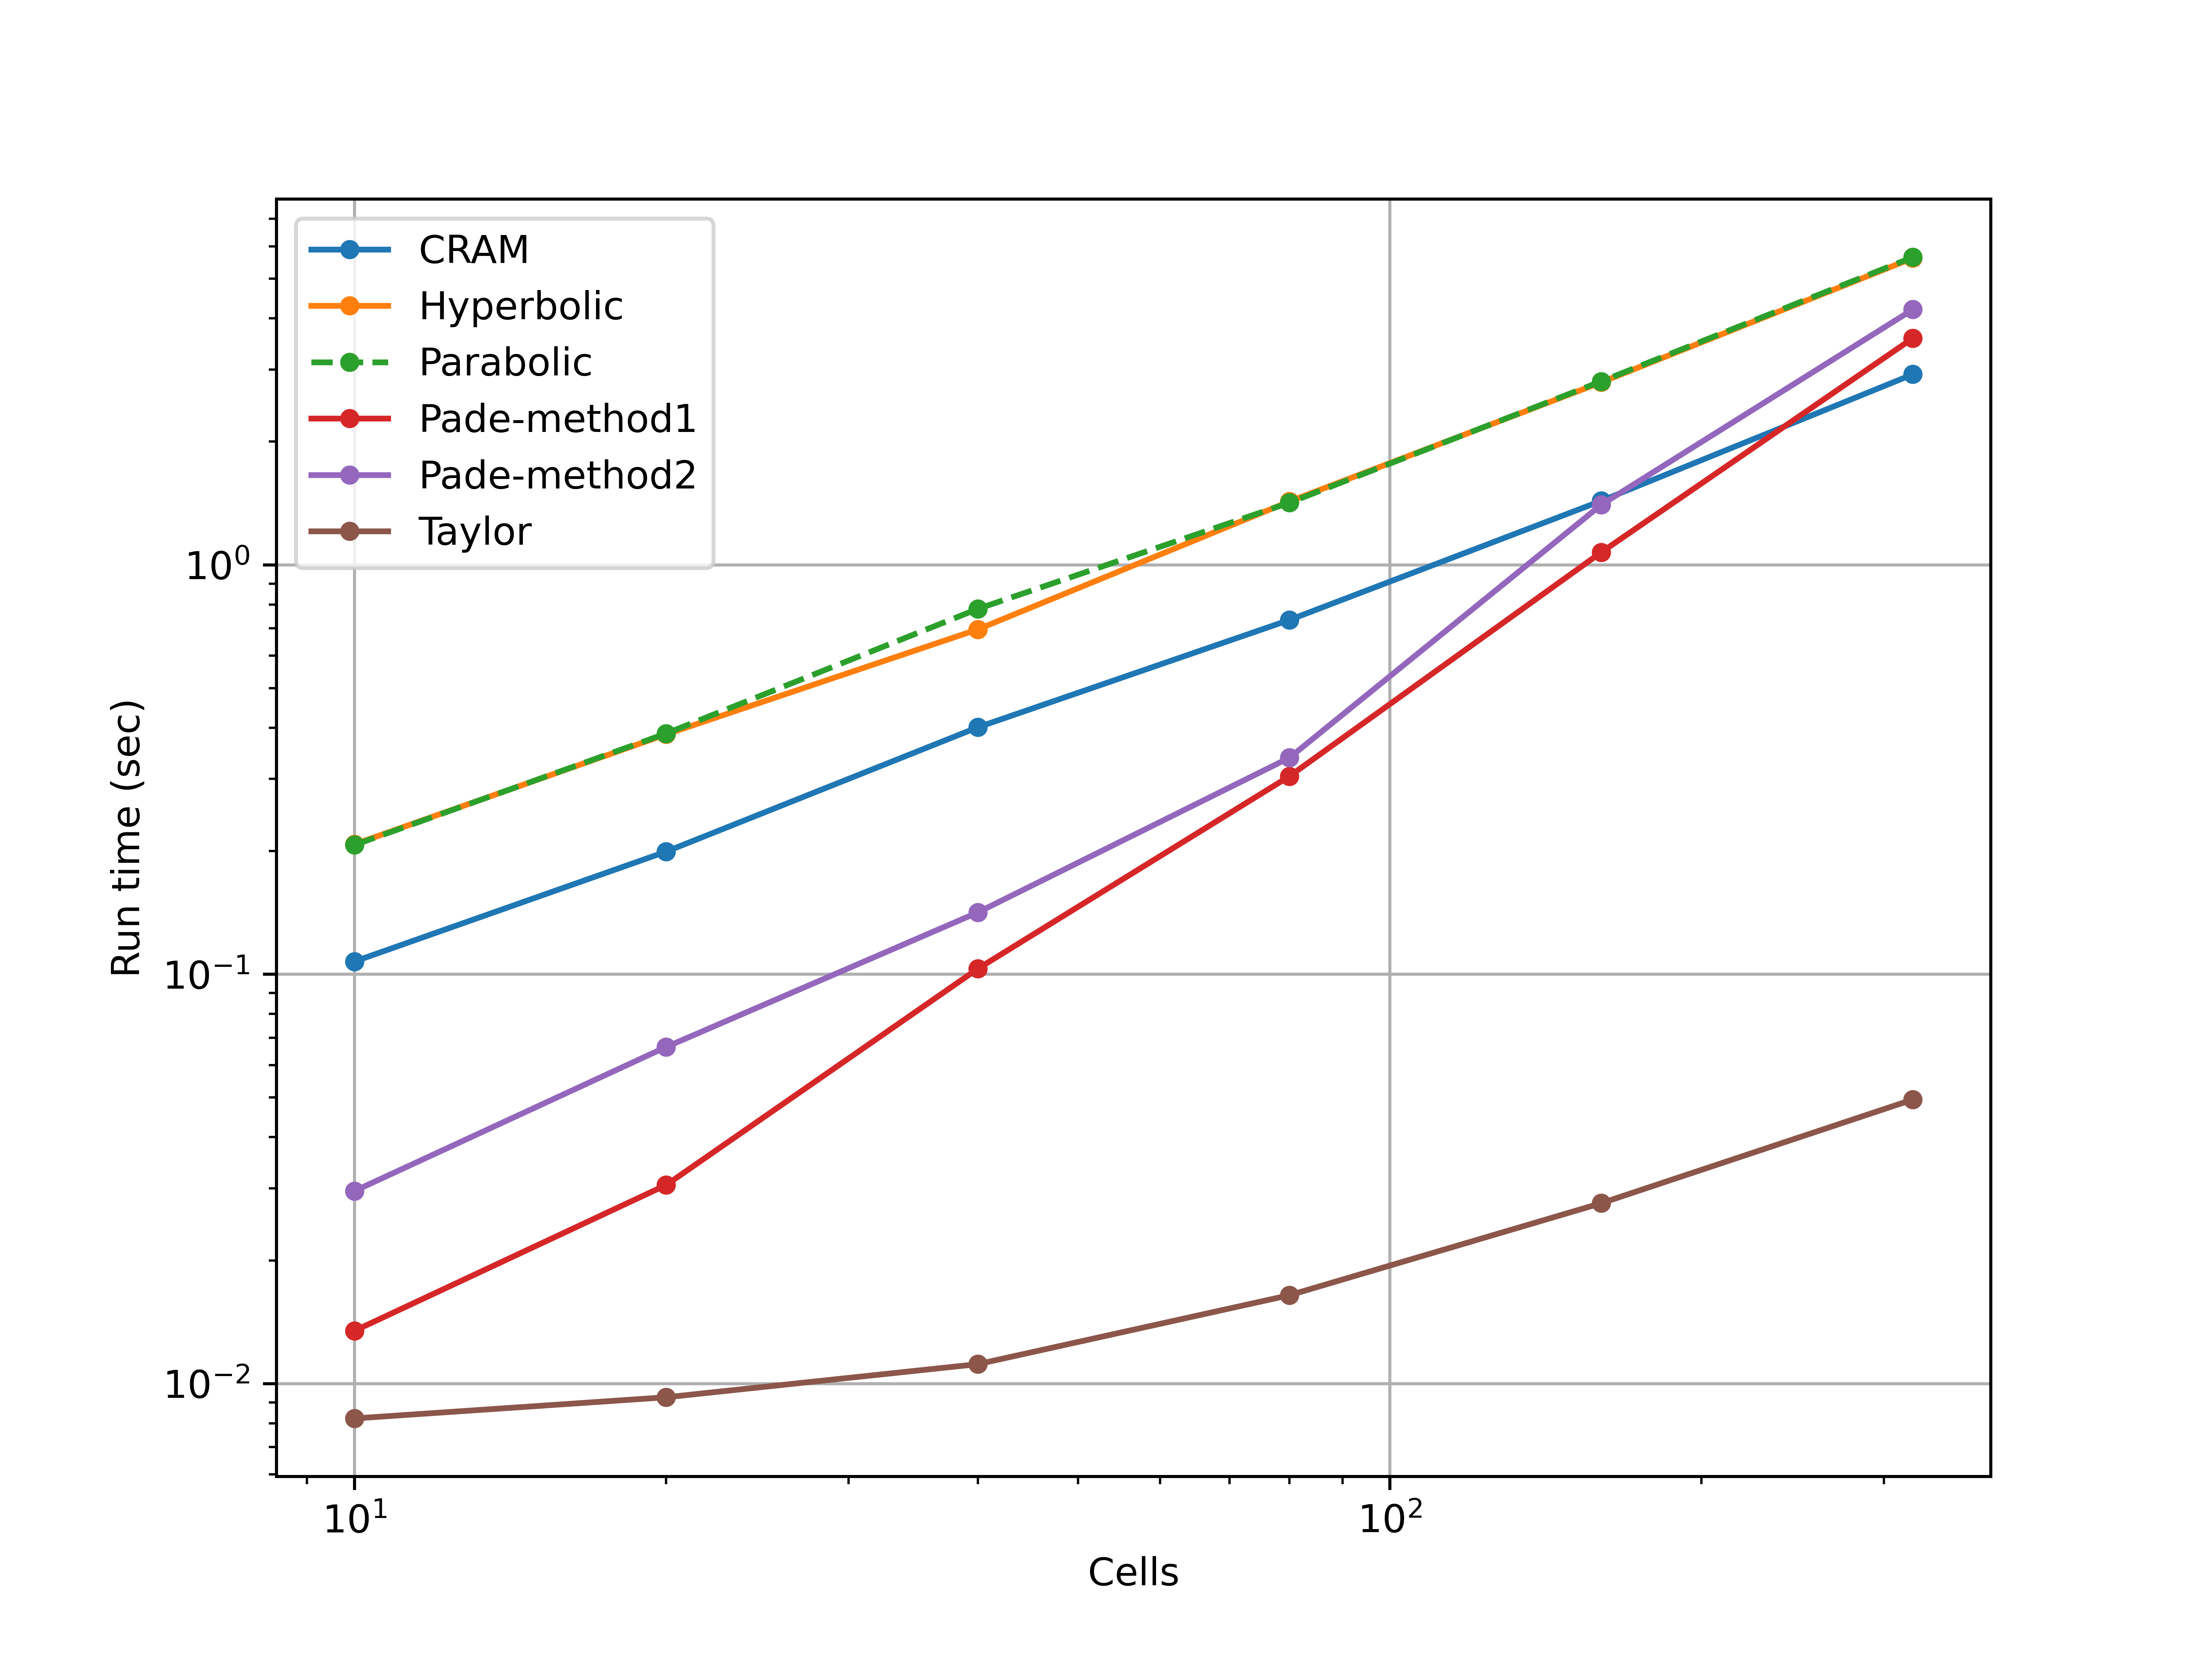
\includegraphics[width=6in]{images/chapter-5/progressionProblems/problem4/problem4Runtimes.png}
    \caption{Problem 4 average run times for each solver, dt = 0.01}
    \label{fig:problem4_runtimes}
\end{figure}

\clearpage

\subsection{Problem 5}
This problem consist on a convection-reaction problem with a single species represented by:

\begin{equation}
    \frac{\partial C}{\partial t} = -v\frac{\partial C}{\partial x} - \lambda C,
\end{equation}

\noindent on the domain $x \in [0,100]$, $t \in [0,20]$ where $v = 2$ and $\lambda = 0.01$. Subject to the following conditions:

\begin{equation}
    C(x, 0) = 1000, \quad C(0,t) = 1000, \quad \frac{dC}{dx}(100, t) = 0.
\end{equation}

\noindent This leads to the analytic solution:

\begin{equation}
C (x,t) = \begin{cases}
  C (x, 0) e^{-\frac{x \lambda _i}{v}}\ , & x < vt \\
  C (x, 0) e^{-t \lambda _i}\ , & x \ge vt
\end{cases}
\end{equation}

This problem is a 1D convection driven flow where the species decays at a constant rate. The solution to this leads to a function that is not smooth, causing the higher order flux limiter functions to reduced to first order accuracy. Figures \ref{fig:problem5_l1error_spatial_results} and \ref{fig:problem5_l1error_time_results} show results for each of the flux limiter functions for the E${}_{1}$ relative error for spatial and temporal discretization. Starting with Figure \ref{fig:problem5_l1error_spatial_results}, each of the flux limiters show about the same convergence rate at the first order upwind function. This agrees with the previous statement about TVD schemes reducing to first order convergence rates for non smooth solutions. While the TVD schemes do not have second order convergence rates, they do increase the accuracy of the solution when compared to first order upwind. This is most prevalent with the Albada limiter, which does show are higher convergence rate with large number of cells and time steps. This limiter also maintains the lowest error for all test shown if Figures \ref{fig:problem5_l1error_spatial_results} and \ref{fig:problem5_l1error_time_results}. Albada also benefits the most from increasing the number of time steps, this is easly seen in Figure \ref{fig:problem5_l1error_time_results}. Figure \ref{fig:problem5_l1error_time_results} also shows that each of the other flux limiter functions are not greatly affected by increasing the number of time steps. For smaller spatial 

\clearpage

\begin{figure}[p]
    \centering
    \includegraphics[width=6in]{images/chapter-5/progressionProblems/problem5/problem5E1ErrorWithSpace.png}
    \caption{Problem 5 relative E${}_{1}$ error with spatial discretization at various time steps}
    \label{fig:problem5_l1error_spatial_results}
\end{figure}

\clearpage

\begin{figure}[p]
    \centering
    \includegraphics[width=6in]{images/chapter-5/progressionProblems/problem5/problem5E1ErrorWithTime.png}
    \caption{Problem 5 relative E${}_{1}$ error with temporal discretization at various number of spatial cells}
    \label{fig:problem5_l1error_time_results}
\end{figure}

\clearpage

\noindent discretizations, increasing the number of time steps does slightly increase the accuracy of the other TVD schemes. Results using the E${}_{\infty}$ and E${}_{2}$ errors are found in Appendix \ref{appen:results} Figures \ref{fig:problem5_linferror_spatial_results}, \ref{fig:problem5_linferror_time_results}, \ref{fig:problem5_l2error_spatial_results} and \ref{fig:problem5_l2error_time_results}. Figure \ref{fig:problem5_linferror_spatial_results} shows that the E${}_{\infty}$ error behaves a little worse than E${}_{1}$, showing different flux limiters achieve minimal error at higher spatial resolution. While Albada is still one of the best, it does not have the lowest error for higher spatial and temporal resolutions. The E${}_{2}$ error, shown in Figure \ref{fig:problem5_l2error_spatial_results}, shows the same behavior as E${}_{1}$. The Albada limiter performs the best and is affected the most by increasing the number of time steps.  

Figure \ref{fig:problem5_l1error_fluxlimiter_convergence_rate} shows convergence rates as a function of time and space. Unlike problem 4, which showed minimal convergence rate in the bottom left corner, these results show the minimal to be in the top left. This corresponds to low spatial and temporal resolution. For each limiter function, the convergence rate is increased by increasing the number of time steps taken. Just as with Figures \ref{fig:problem5_l1error_spatial_results} and \ref{fig:problem5_l1error_time_results}, Figure \ref{fig:problem5_l1error_fluxlimiter_convergence_rate} shows the the Albada limiter has the highest convergence rate, reaching a sweet spot at 80 cells and 400 time steps. Figures \ref{fig:problem5_linferror_fluxlimiter_convergence_rate} and \ref{fig:problem5_l2error_fluxlimiter_convergence_rate} shows convergence rates for E${}_{\infty}$ and E${}_{2}$ errors. The $l_{\infty}$ error shows high convergence rates for for low cells and high time steps for all but the Albada and Min-Mod limiters. The E${}_{2}$ error shows high convergence rates for high time steps, generally reaching a plateau as the number of cells in increased.

Figure \ref{fig:problem5_l1error_coefficient_changes} shows how the problem behaves as a function of $v$ and $\lambda$. These coefficients are changed to induce and reaction or velocity dominated system. In a reaction dominated system, all of the flux limiter functions converge to a single point. This is because the accuracy of the solution is dominated by the integration of the reaction rate of the time interval. As the velocity is increased, the flux limiters begin to diverge to difference accuracy's. The Albada limiter diverges the most, decreasing the error 2 orders of magnitude below all the others. What is also interesting is that the error follows a hump shape, increasing up until it reaches a max value where the coefficient are the same. After this, the error decreases. This is also the point where the Albada separates from the rest. 

Figure \ref{fig:problem5_runtimes} show how each of the solvers scale with number of cells. On the log-log scale, the Cauchy and Taylor solvers scale linearly while the Pad\'e solvers begin low then increase 

\clearpage

\begin{figure}[p]
    \centering
    \includegraphics[width=6in]{images/chapter-5/progressionProblems/problem5/problem5E1FluxLimiterConvergenceRate.png}
    \caption{Problem 5 flux limiter relative E${}_{1}$ spatial convergence rate using absolute error}
    \label{fig:problem5_l1error_fluxlimiter_convergence_rate}
\end{figure}

\clearpage

\begin{figure}[p]
    \centering
    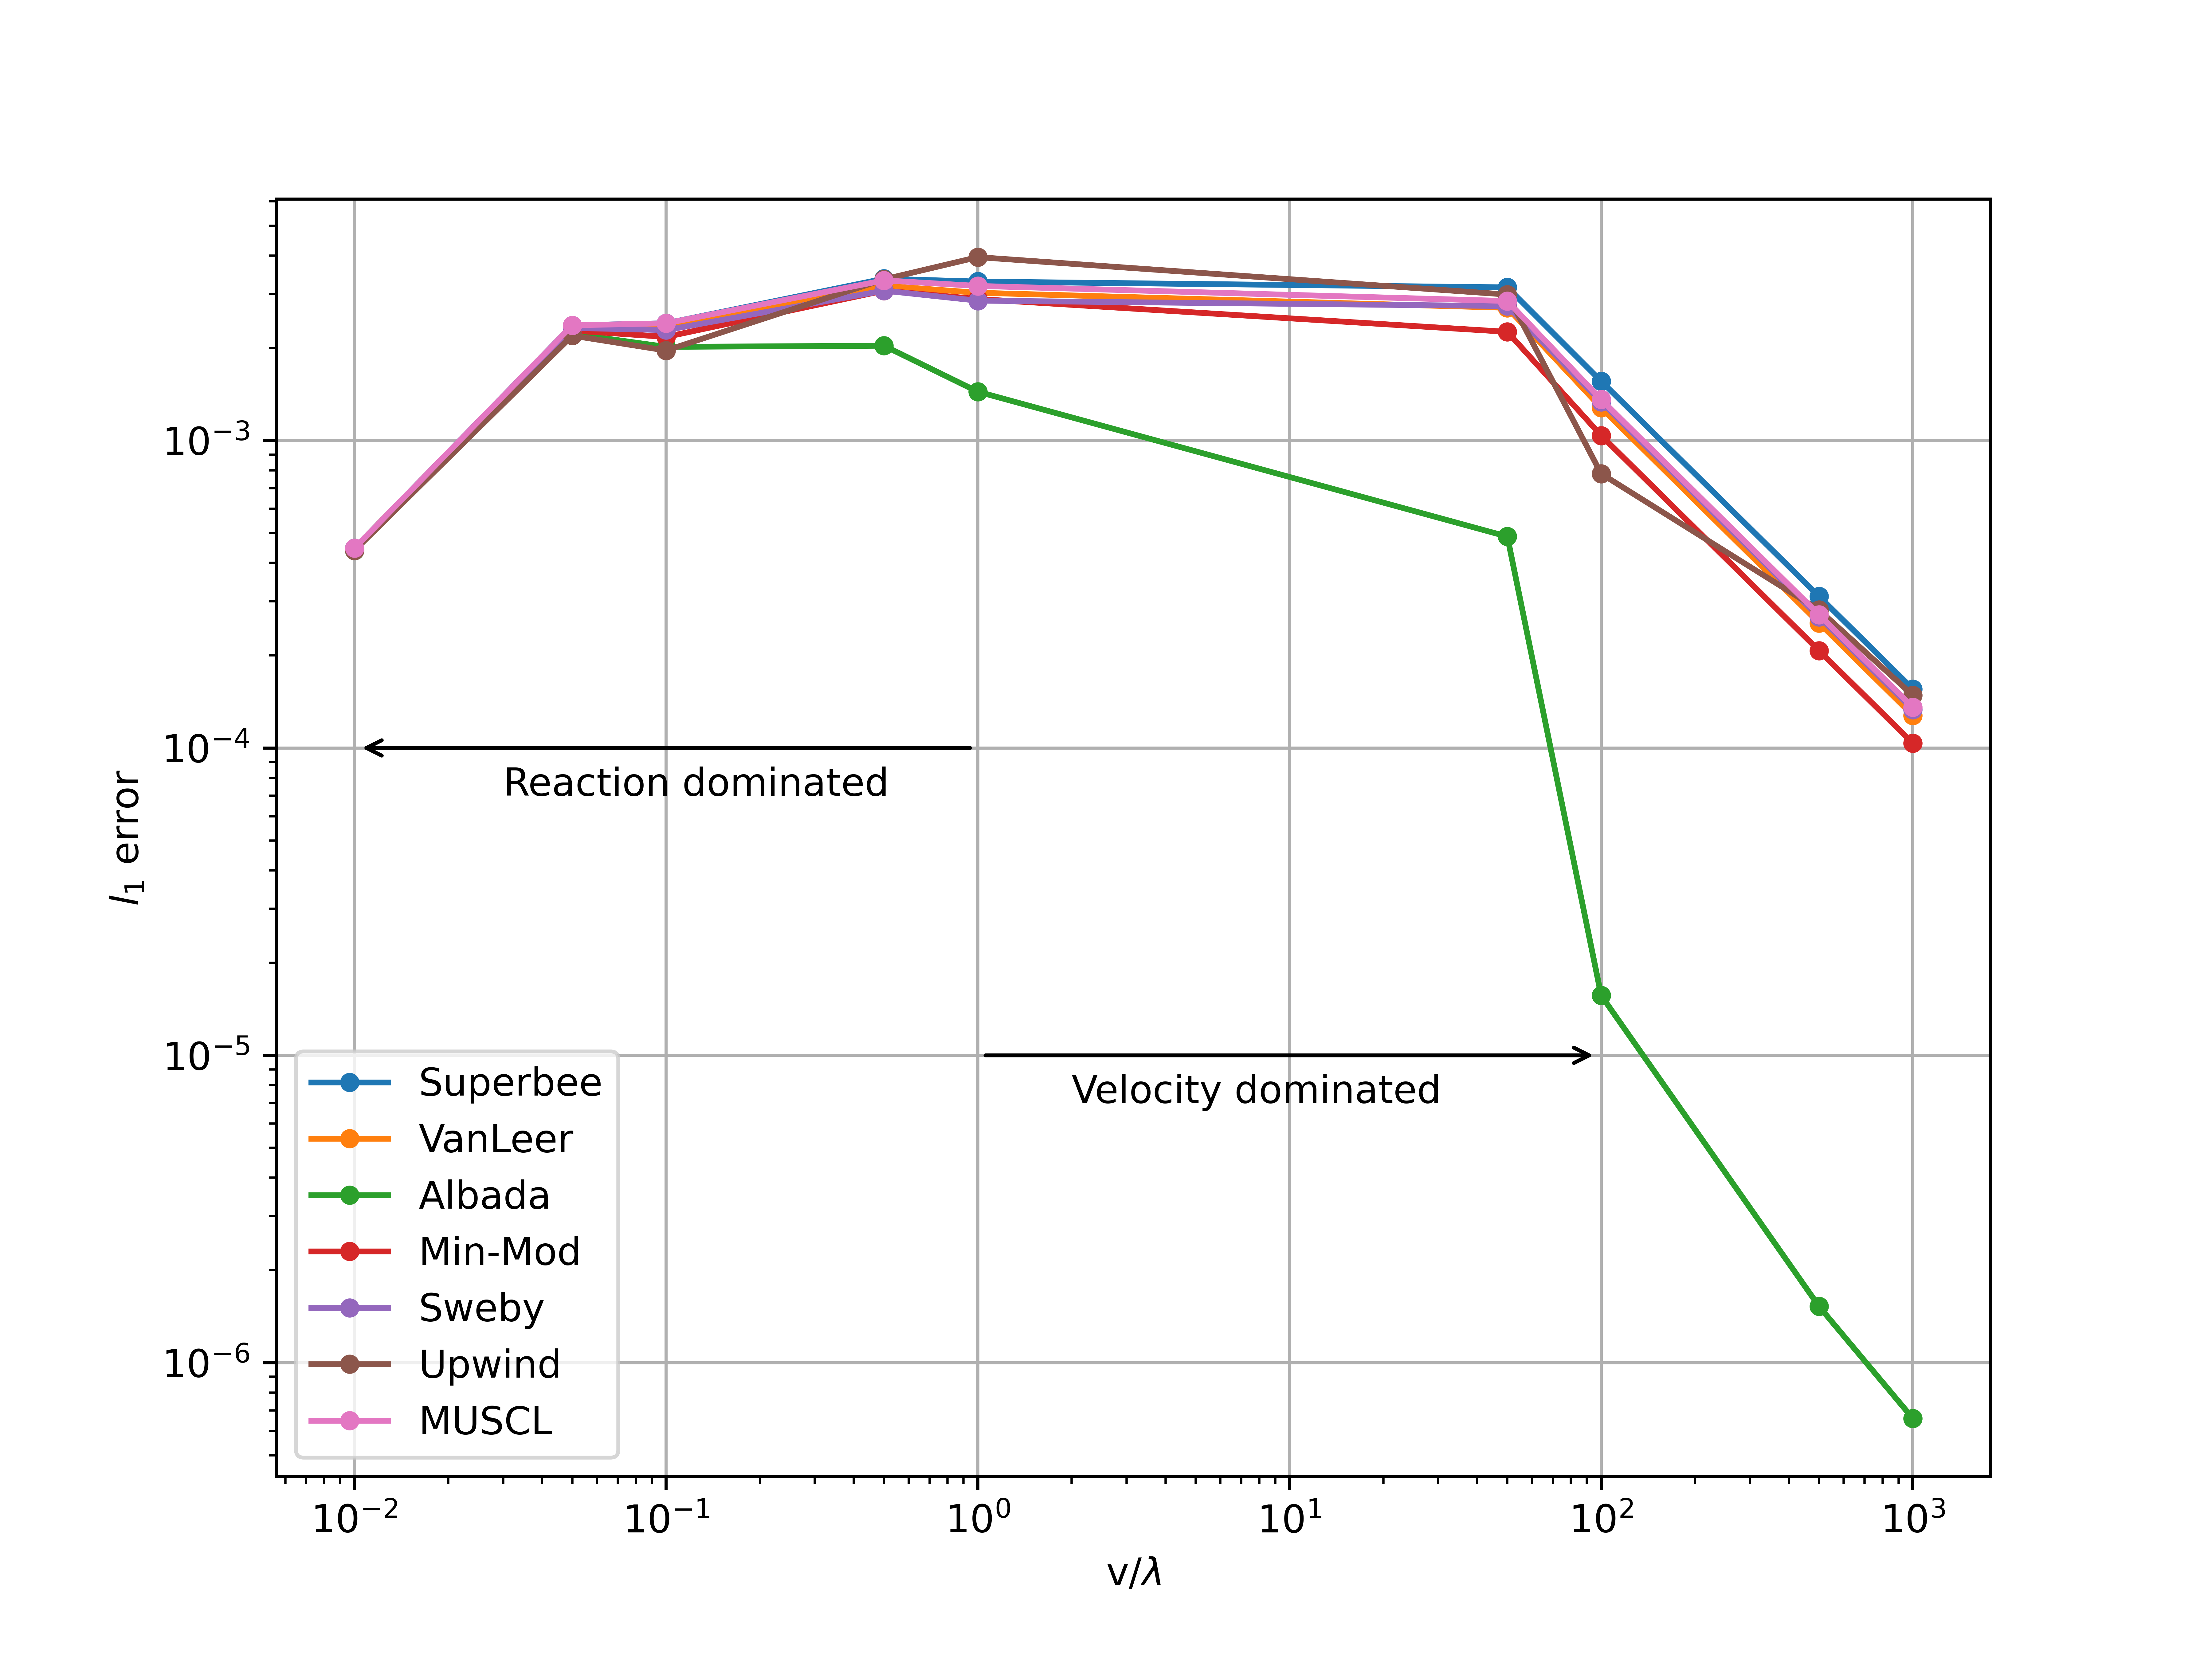
\includegraphics[width=6in]{images/chapter-5/progressionProblems/problem5/problem5CoefficientChanges.png}
    \caption{Problem 5 flux limiter relative E${}_{1}$ behavior with coefficient changes using absolute error}
    \label{fig:problem5_l1error_coefficient_changes}
\end{figure}

\clearpage

\begin{figure}[p]
    \centering
    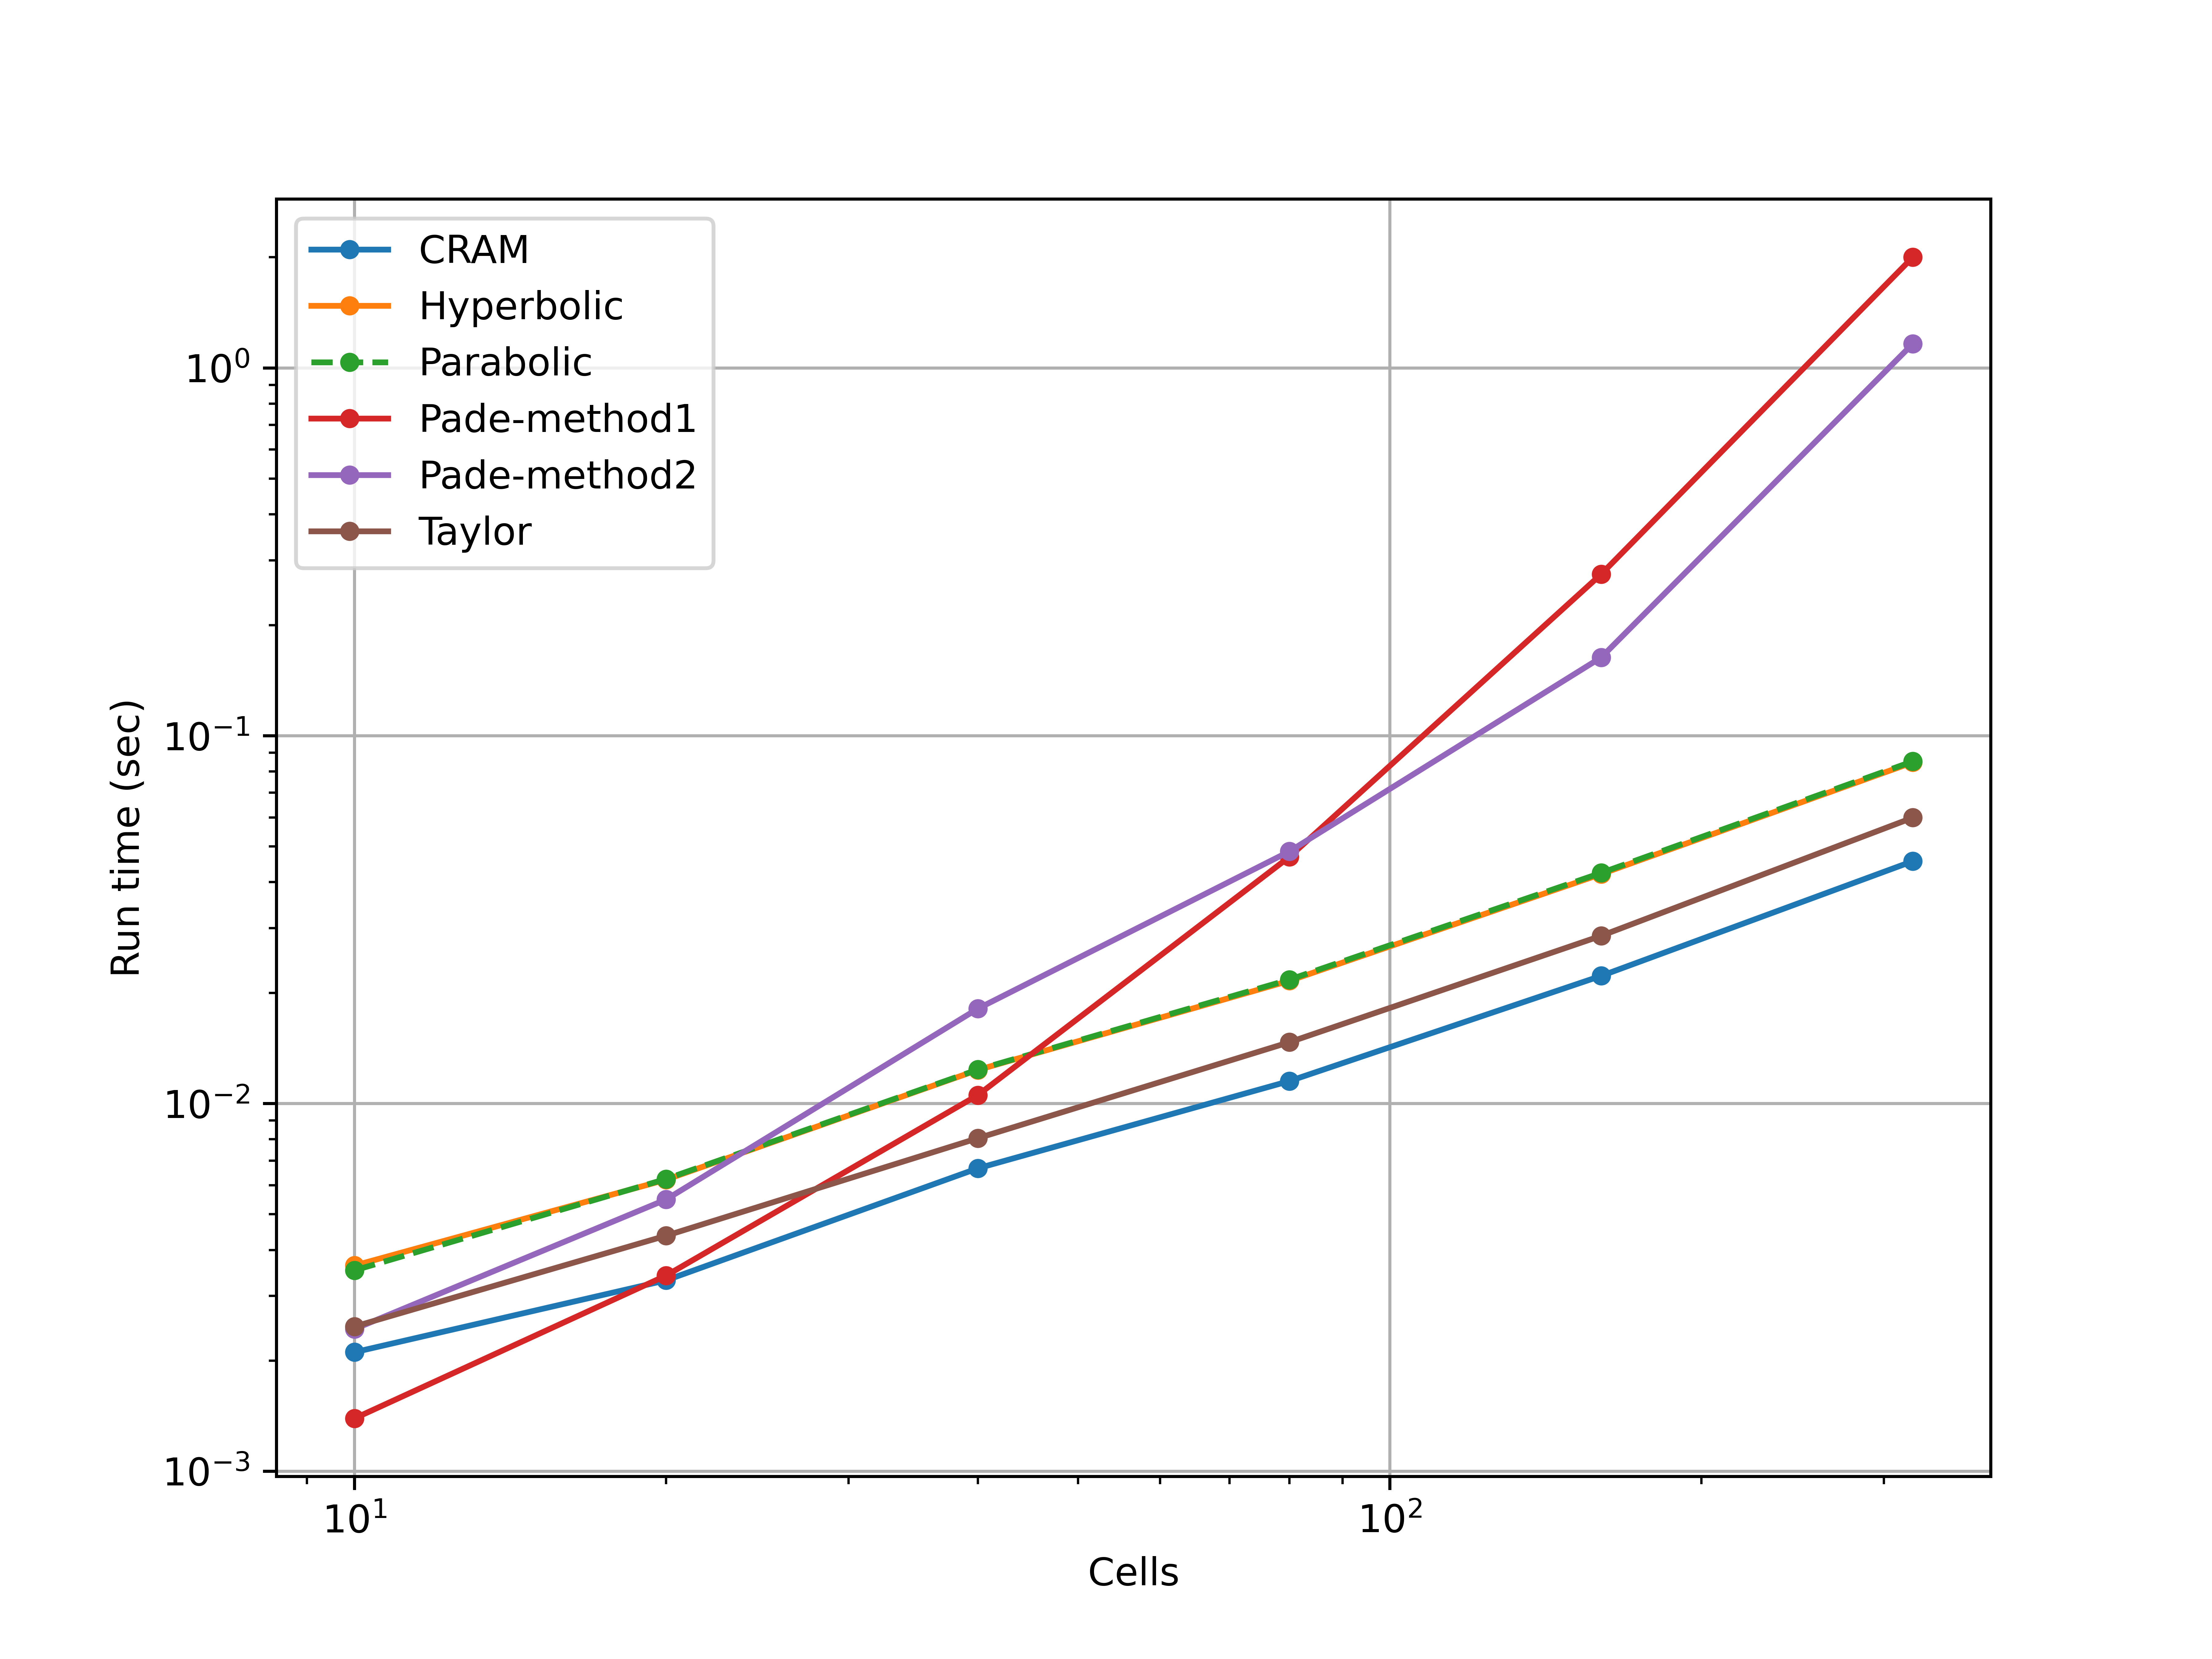
\includegraphics[width=6in]{images/chapter-5/progressionProblems/problem5/problem5Runtimes.png}
    \caption{Problem 5 average run times for each solver, dt = 0.1}
    \label{fig:problem5_runtimes}
\end{figure}

\clearpage

\noindent to a point above the others. This indicates that the Pad\'e solvers scale much more poorly. As with problem 3, the Cauchy solvers did show instability. These instabilities were also remedied by increasing the order of the method and by adding substeps. 

\subsection{Problem 6}
This is an extension of problem 6 with two species, one that exist in the liquid and one on the wall. The species in the liquid transports and depositions on the wall where it sticks and does not move. In libowski this is accomplished by excluding the loop which adds the convection contribution to the wall species. This system is represented by:

\begin{equation}
\setlength{\jot}{15pt}
\begin{split}
    &\frac{\partial C_{l}}{\partial t} = -v\frac{\partial C_{l}}{\partial x} - \frac{kA}{V} C_{l}, \\
    &\frac{\partial C_{w}}{\partial t} = \frac{kA}{V} C_{l},
    \label{eq:problem6}
\end{split}
\end{equation}

\noindent on the domain $x \in [0,100]$, $t \in [0, 20]$ where $v = 2$ and $kA/V = \lambda = 0.01$. Subject to the following conditions:

\begin{equation}
\setlength{\jot}{15pt}
\begin{split}
    C_{l}(x, 0) = 1000, \quad C_{l}(0,t) = 1000, \quad \frac{dC_{l}}{dx}(100, t) = 0, \\
    C_{w}(x, 0) = 0, \quad C_{w}(0,t) = 0, \quad \frac{dC_{l}}{dx}(100, t) = 0. \\
\end{split}
\end{equation}

\noindent Let $\lambda = kA/V$, equation \ref{eq:problem6} the following solution:

\begin{equation}
C_{l} (x,t) = \begin{cases}
  C_{l} (x, 0) e^{-\frac{x \lambda _i}{v}}\ , & x < vt \\
  C_{l} (x, 0) e^{-t \lambda _i}\ , & x \ge vt
\end{cases}
\end{equation}

\begin{equation}
C_{w} (x,t) = \begin{cases}
  C_{l} (x, 0) \Big( 1 - e^{-\frac{x \lambda _i}{v}} + \lambda \big(t - x/v\big)e^{-\lambda x/v} \Big)\ , & x < vt \\
  C_{l} (x, 0) \Big( 1 - e^{-t \lambda _i}\Big)\ , & x \ge vt
\end{cases}
\end{equation}

This problem is conducted in the same manor as problem 4 and 5. But unlike problem 4, this problem has a discontinuous solution. Figures \ref{fig:problem6_l1error_spatial_results} and  \ref{fig:problem6_l1error_time_results} shows results for the E${}_{1}$ error as a function of time and space. These results shows the same behavior for each of the flux limiters that was shown in problem 4. The only difference is the error is slightly higher in this problem. Again, the Albada flux limiter showes the lowest over all error and does show the most improvement from increasing the number of time steps. Figure \ref{fig:problem6_linferror_spatial_results} and \ref{fig:problem6_linferror_time_results} shows that the E${}_{\infty}$ error follows the same shape from problem 5. For high dt, each of the flux limiters seem to converge to the same solution. As the time step size is decreased, each flux limiter begins to separate, with Albada acheiving the lowest error for low dt and dx. Figure \ref{fig:problem6_linferror_time_results} shows that for a high dx, increasing the number of time steps causes most of the high order flux limiter functions to become worst. As dx becomes lower, all of the high order functions become more accurate until they reach a point where decreasing dt does not affect the solution. The Albada limiter however, increases its accuracy as dt decreases for all dx values. Figures \ref{fig:problem6_l2error_spatial_results} and \ref{fig:problem6_l2error_time_results} show that the E${}_{2}$ also behaves the same in problems 5 and 6. For a low number of cells, each of the limiter functions converge to a similar solution, with the Albada limiter out performing the rest. 

Figure \ref{fig:problem6_l1error_fluxlimiter_convergence_rate} shows the spatial convergence rate as a function of space and time. This Figure shows the same convergence behavior seen in problem 5, but with slightly different values. In this case, the Albada limiter shows a higher convergence rate, while each of the other limiters seem to have higher convergence rates for higher dt. As the number of steps is increased the convergence rates are higher in problem 5. Figures \ref{fig:problem6_linferror_fluxlimiter_convergence_rate} and \ref{fig:problem6_l2error_fluxlimiter_convergence_rate} show the spatial convergence rates for the E${}_{\infty}$ and E${}_{2}$. Both of these Figures show the same trend that was seen in problem 5. The E${}_{\infty}$ error shows low convergence rates for the Albada and Min-Mod limiters, while the other limiters have high convergence rates for both low dt and dx. The E${}_{2}$ error shows higher convergence rates for all limiters for both low dt and dx. 

Figure \ref{fig:problem6_l1error_coefficient_changes} shows E${}_{1}$ error with changes in the problem coefficients. This Figure shows almost the exact same behavior that was seen in problem 5. In a reaction dominated system, all limiters converge to the same solution. As the velocity is increased, each of the limiters 

\clearpage

\begin{figure}[p]
    \centering
    \includegraphics[width=6in]{images/chapter-5/progressionProblems/problem6/problem6E1ErrorWithSpace.png}
    \caption{Problem 6 relative E${}_{1}$ error with spatial discretization at various time steps}
    \label{fig:problem6_l1error_spatial_results}
\end{figure}

\clearpage

\begin{figure}[p]
    \centering
    \includegraphics[width=6in]{images/chapter-5/progressionProblems/problem6/problem6E1ErrorWithTime.png}
    \caption{Problem 6 relative E${}_{1}$ error with temporal discretization at various number of spatial cells}
    \label{fig:problem6_l1error_time_results}
\end{figure}

\clearpage

\begin{figure}[p]
    \centering
    \includegraphics[width=6in]{images/chapter-5/progressionProblems/problem6/problem6E1FluxLimiterConvergenceRate.png}
    \caption{Problem 6 flux limiter relative E${}_{1}$ spatial convergence rate}
    \label{fig:problem6_l1error_fluxlimiter_convergence_rate}
\end{figure}

\clearpage

\begin{figure}[p]
    \centering
    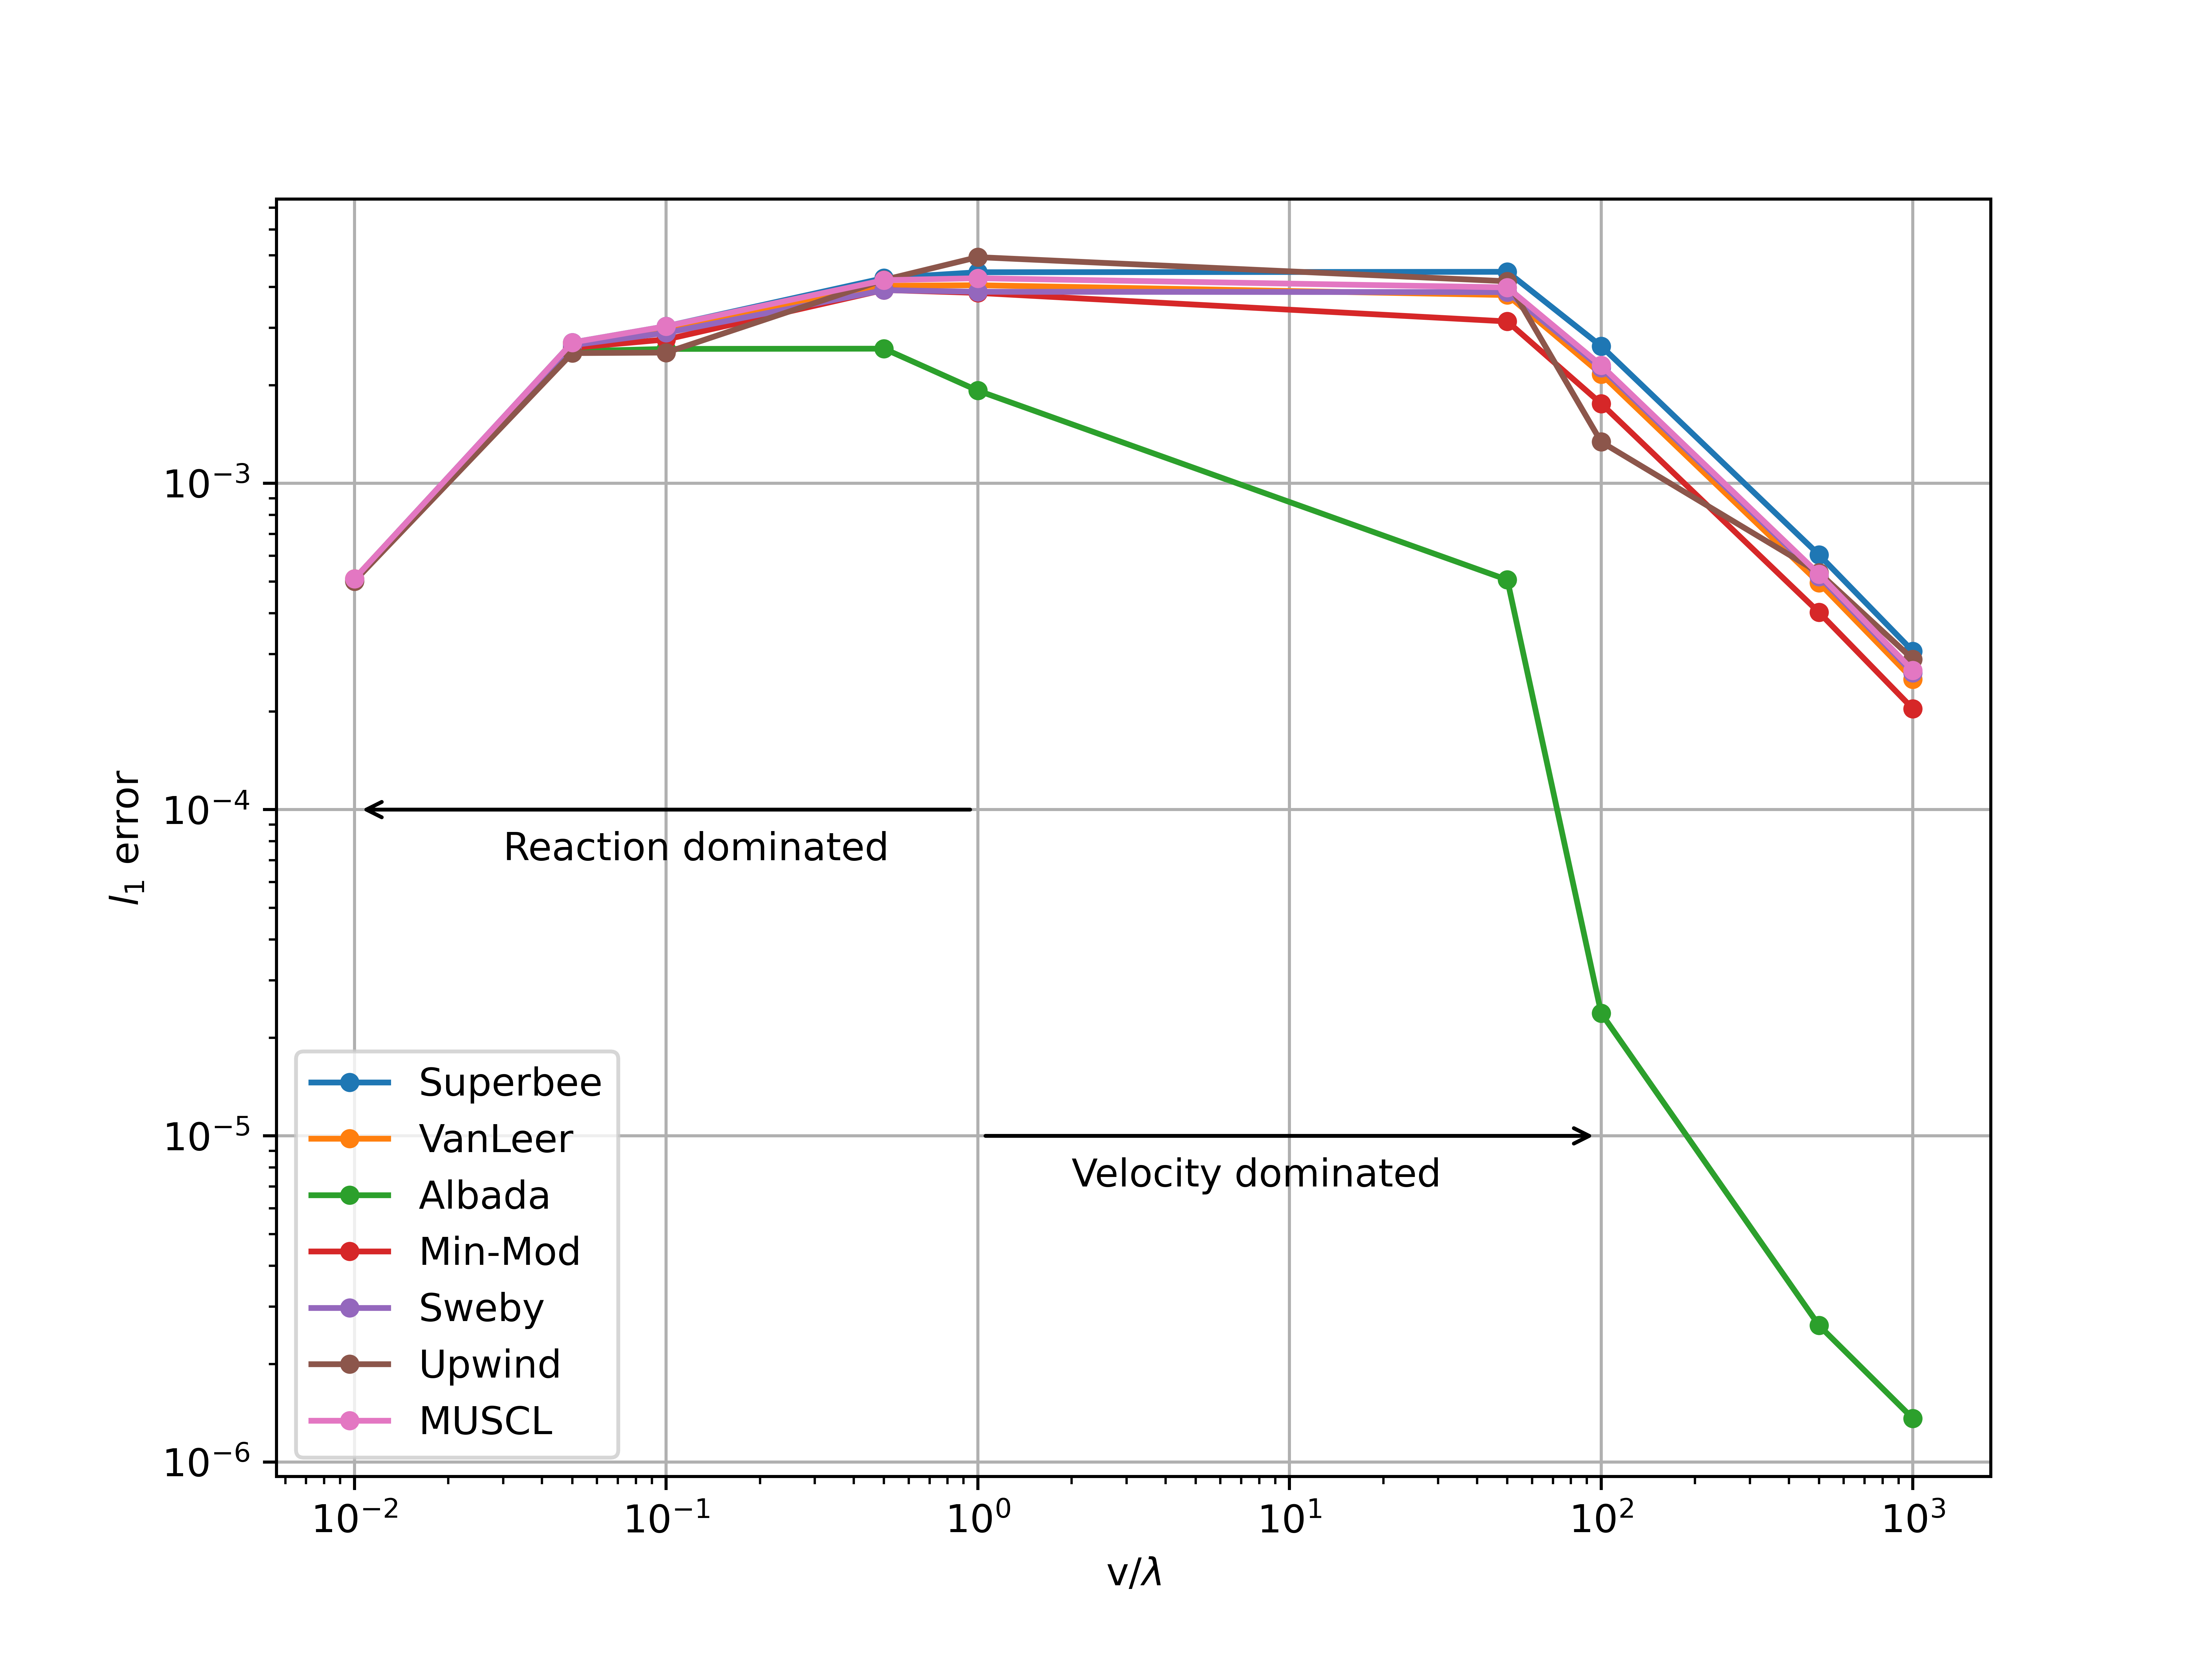
\includegraphics[width=6in]{images/chapter-5/progressionProblems/problem6/problem6CoefficientChanges.png}
    \caption{Problem 6 flux limiter relative E${}_{1}$ behavior with coefficient changes}
    \label{fig:problem6_l1error_coefficient_changes}
\end{figure}

\clearpage

\noindent separate, with the Albada limiter performing the best. Figure \ref{fig:problem6_runtimes} shows run times for this problem behave in a similar way to problem 5. However in problem 6, the Taylor, Hyperbolic and Parabolic solvers have almost the same run times.

\subsection{Problem 7}
This problem models the primary uranium isotopes along with Pu-239 and Np-239 in a system which contains a neutron flux. Coefficients in the transition matrix include source and sink terms from both neutron induced reactions and radioactive decay. This system is represented by:


\begin{equation}
\frac{d C_i}{dt} = \sum^9_{j = 1} A_{ij} C_j (x, t)
\end{equation}

\begin{equation}
i = \begin{dcases}
  1 , & \text{$^{233}$U}  \\
  2 , & \text{$^{234}$U}  \\
  3 , & \text{$^{235}$U}  \\
  4 , & \text{$^{236}$U}  \\
  5 , & \text{$^{237}$U}  \\
  6 , & \text{$^{238}$U}  \\
  7 , & \text{$^{239}$U}  \\
  8 , & \text{$^{239}$Pu} \\
  9 , & \text{$^{239}$Np} \\
\end{dcases}
\end{equation}

\noindent On the domain from $t \in [0, 500]$ subject to the following neutron flux $\phi = 1e13$ n/cm$^2/$/s. Each isotope is given an initial concentration of $C_{i, 0} = 1e10$ atoms/cm$^2$. The transition matrix is built using information from the SCALE ORIGEN library. The analytical solution is given by the exponential of the transition matrix:

\begin{equation}
   \boldsymbol{C}(t) = e^{\boldsymbol{A}t}, 
\end{equation}

\clearpage

\begin{figure}[p]
    \centering
    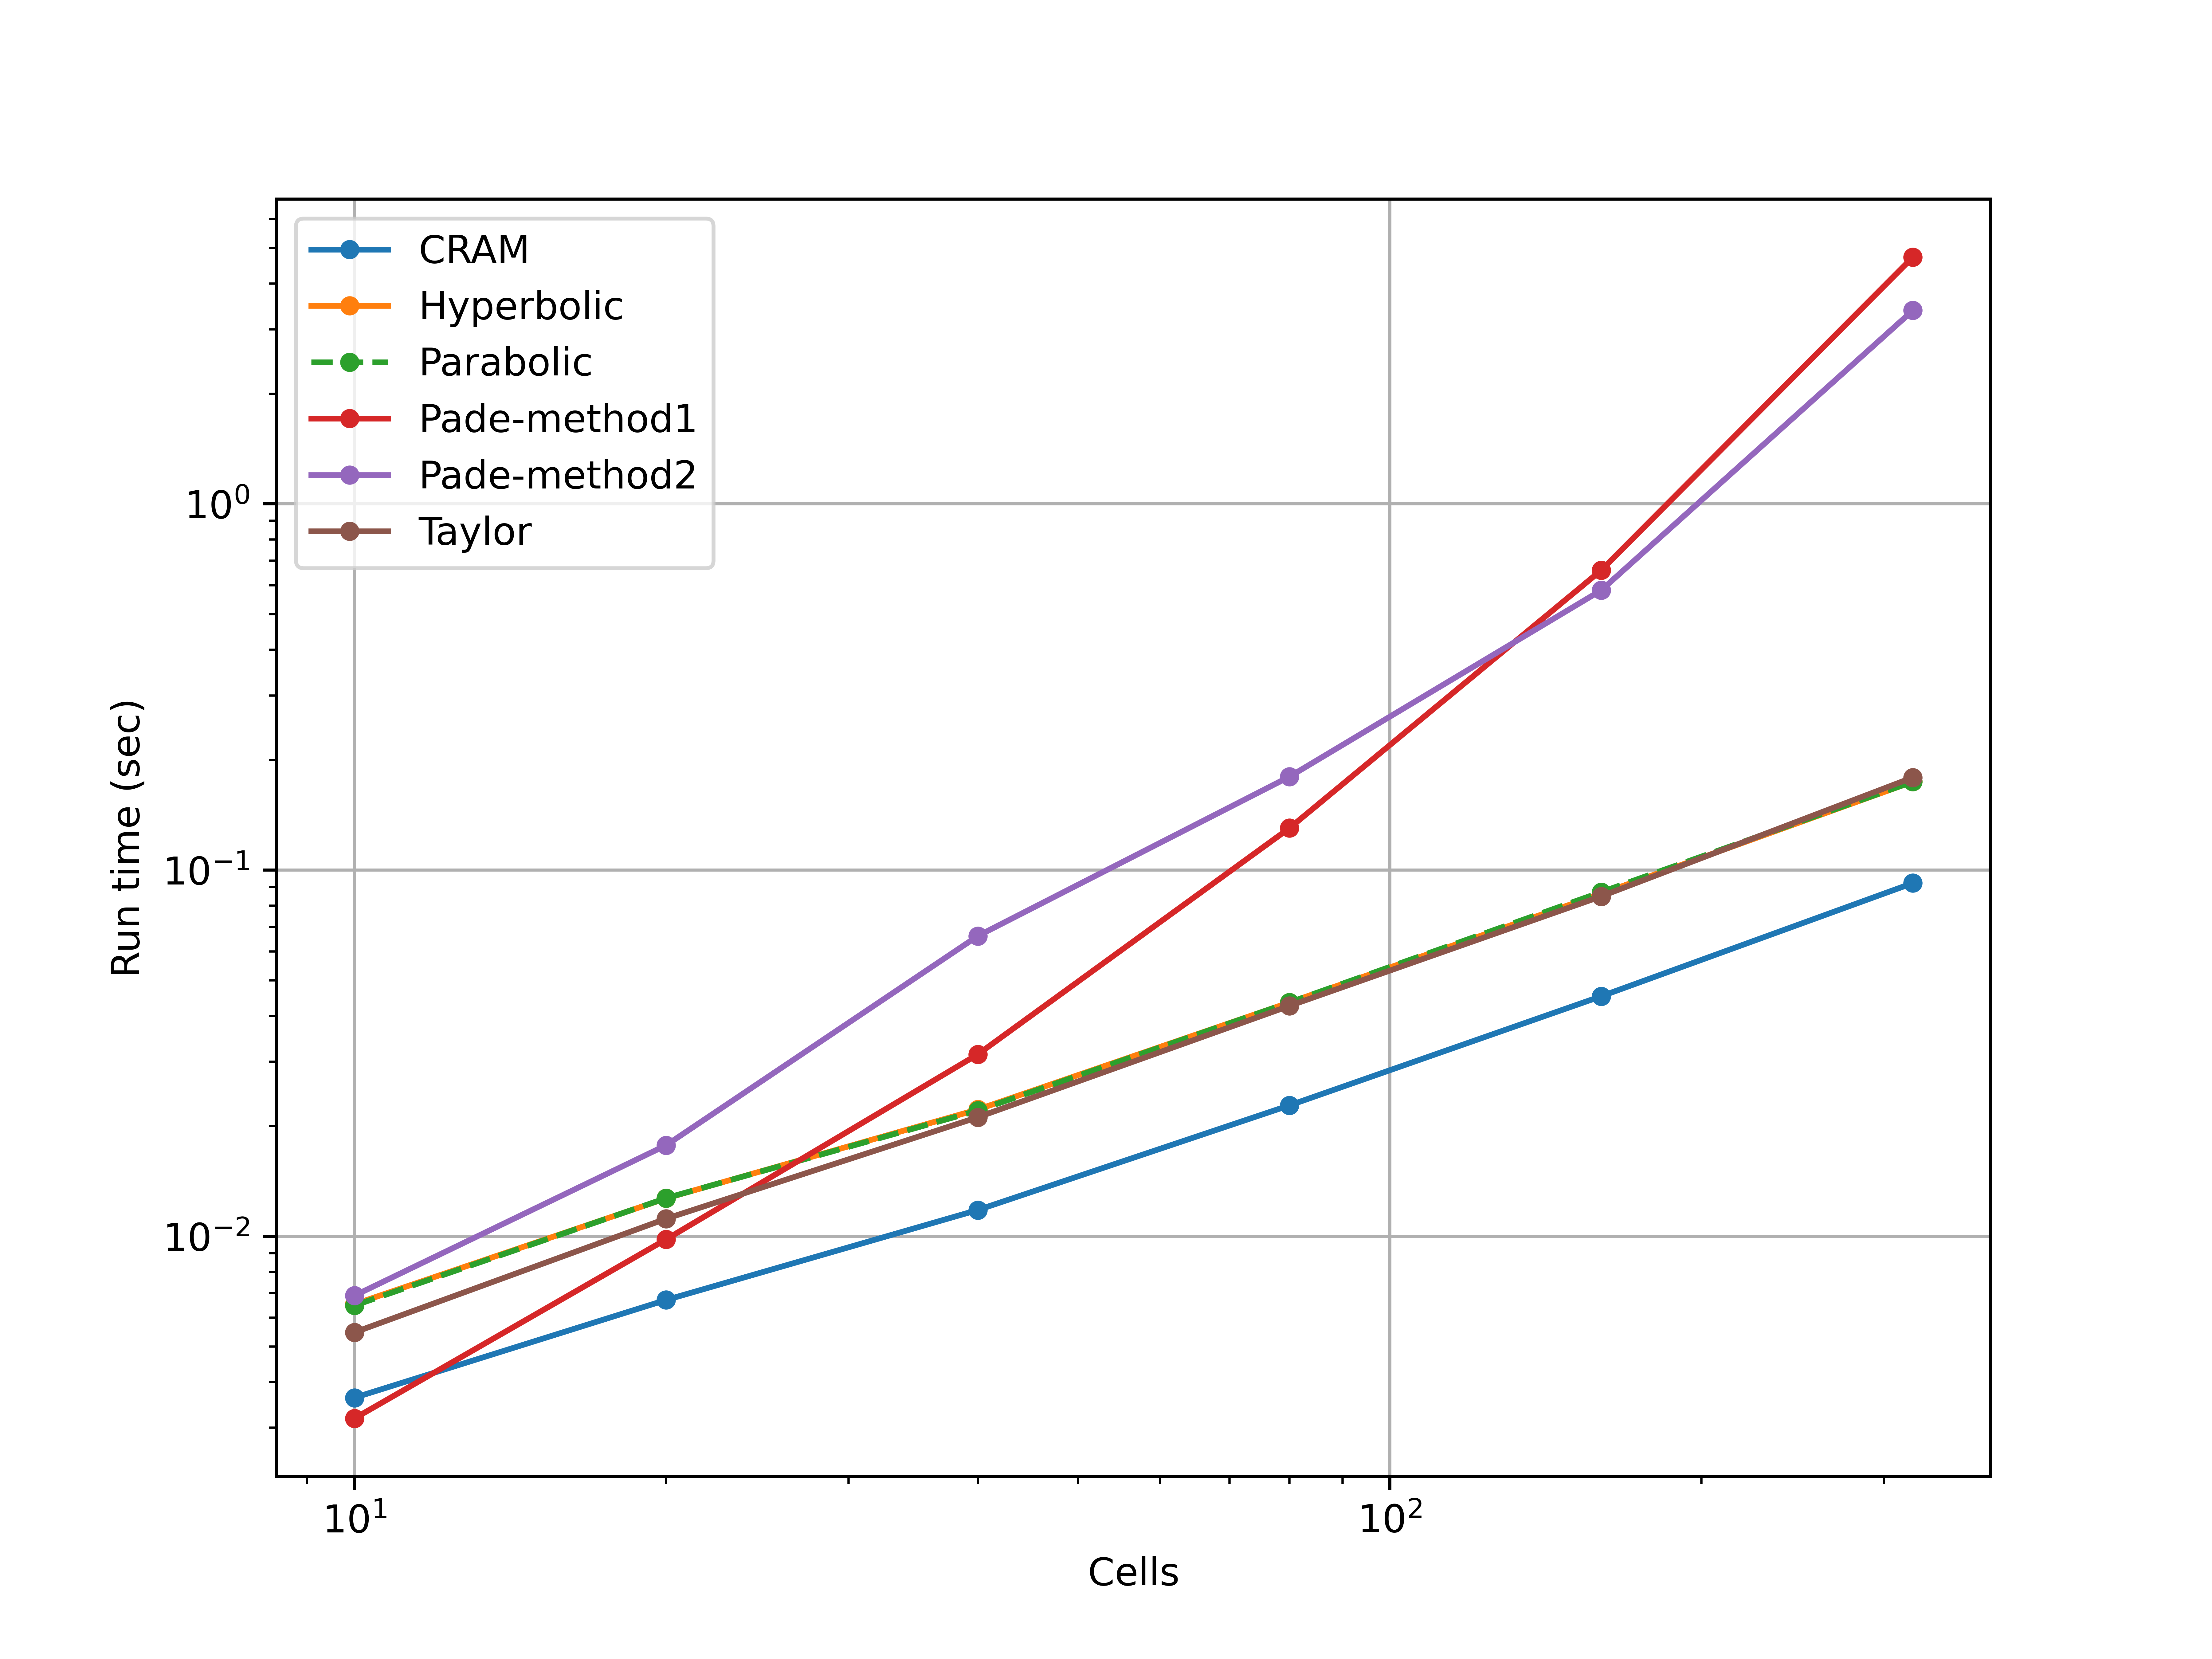
\includegraphics[width=6in]{images/chapter-5/progressionProblems/problem6/problem6Runtimes.png}
    \caption{Problem 6 average run times for each solver, dt = 0.1}
    \label{fig:problem6_runtimes}
\end{figure}

\clearpage

\noindent where $\boldsymbol{C}$ is a vector of isotope concentrations. The solution is calculated using in MATLAB using the method previously described. This solution is plotted in Figure \ref{fig:problem7_solution}, with a zoomed in portion showing the solution for a number of the isotopes are very close. 


This problem offers a good example of how sub-stepping can be utilized in improving the solution for Cauchy solvers.  Results of the sub-stepping for the Cauchy solvers are shown in Figure \ref{fig:problem7_E1_error_with_steps} at the 50-day time step mark. Surprisingly, CRAM started out with the largest E${}_{1}$ relative error. With just 2 substeps, the error from all Cauchy solvers dropped by many orders of magnitude. Past 4 substeps, the errors begin to compound from an inaccurate initial condition. While the behavior in this system shows that 6 is the optimal number of sub-steps for the CRAM and Hyperbolic solvers and 2 for the Parabolic solver. Error behavior for E${}_{\infty}$ and E${}_{2}$ are shown in Appendix \ref{appen:results}, Figures \ref{fig:problem7_Einf_error_with_steps} and \ref{fig:problem7_E2_error_with_steps}. Figure \ref{fig:problem7_Einf_error_with_steps} shows the same trend but with a minimal value at 4 steps instead of 6 for CRAM and Hyperbolic. Figure \ref{fig:problem7_E2_error_with_steps} shows the same behavior that was seen with the E${}_{1}$ error. 

Results for the decay transition matrix are shown in Figure \ref{fig:problem7_E1_error_with_steps4}, where each Cauchy solver was run with 4 substeps. Both the CRAM and hyperbolic solvers outperformed the other solvers. The parabolic solver, the Taylor solver, and the Pad\'e-method 1 solver all performed about the same. The Pad\'e-method 2 solver performed the worst, but the E${}_{1}$ relative error was still below $10^{-9}$ over the solution domain. Results for E${}_{\infty}$ and E${}_{2}$ are shown in Figures \ref{fig:problem7_Einf_error_with_steps4} and \ref{fig:problem7_E2_error_with_steps4}, these results show the same trends seen in Figure \ref{fig:problem7_E1_error_with_steps4}. 


Run times for all of these solvers were quite fast and are shown in Table \ref{tab:problem7_run_times}; Cauchy solvers are shown for 4 sub-steps. For a test as small as the one analyzed here, all run times were remarkably fast. While the $l_{l}$ matrix norm is ~2,100 for the time step size and requires a notable amount of scaling, the problem was small enough that it did not increase the run times for series solvers. 

Eigenvalues for this problem are shown in Figure \ref{fig:problem7_eigenvalues}, while most have zero for the imaginary parts there are two which have non zero elements. However, these eigenvalues are still clustered extremely close to the zero axis and do not affect the accuracy of the Cauchy solvers by themselves. While the accuracy of the Cauchy solvers are not affected by the 

\clearpage

\begin{figure}[p]
    \centering
    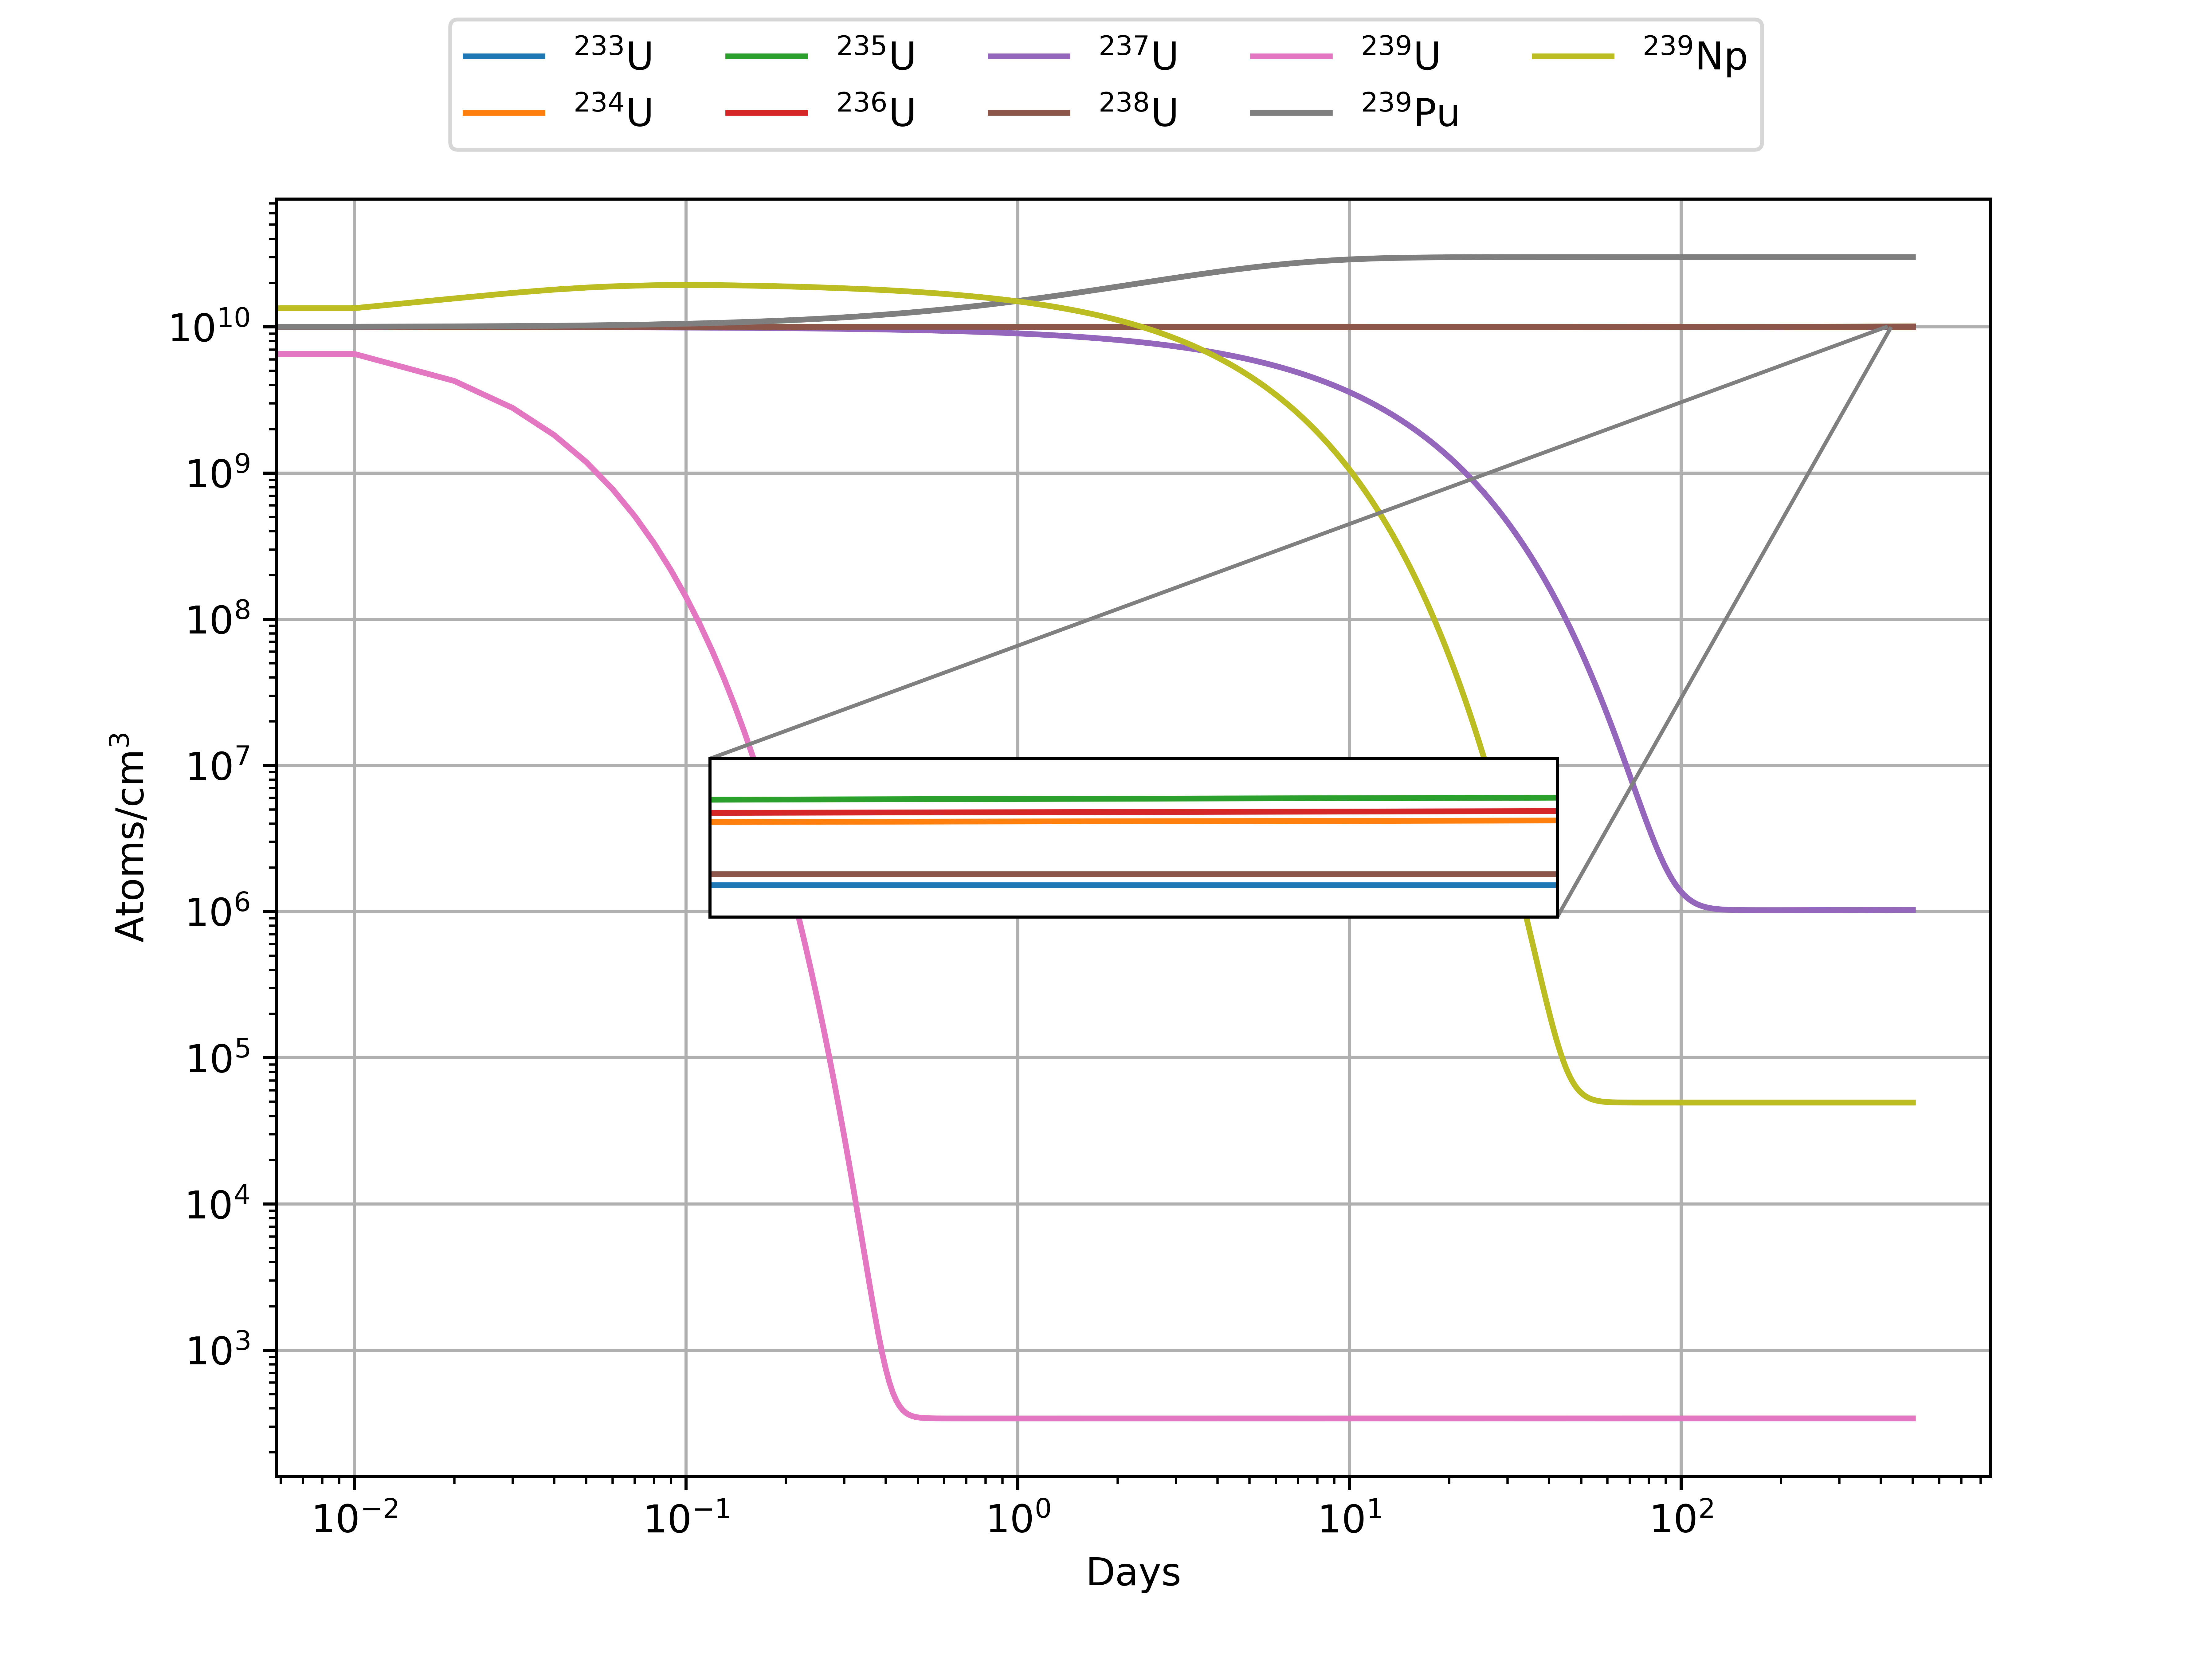
\includegraphics[width=6in]{images/chapter-5/progressionProblems/problem7/problem7soltution.png}
    \caption{Problem 7 solution}
    \label{fig:problem7_solution}
\end{figure}

\clearpage

\begin{figure}[p]
    \centering
    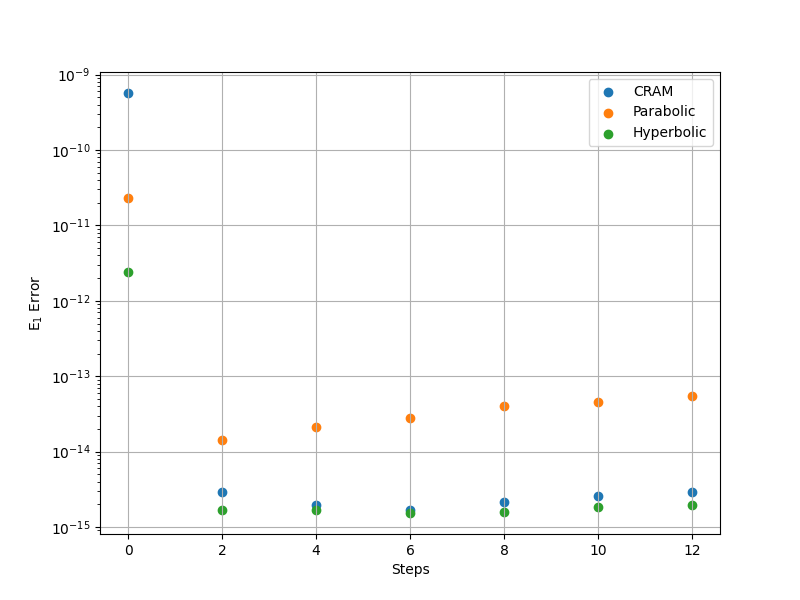
\includegraphics[width=6in]{images/chapter-5/progressionProblems/problem7/problem7E1ErrorWithSteps.png}
    \caption{Problem 7 E${}_{1}$ relative error with sub-steps}
    \label{fig:problem7_E1_error_with_steps}
\end{figure}

\clearpage

\begin{figure}[p]
    \centering
    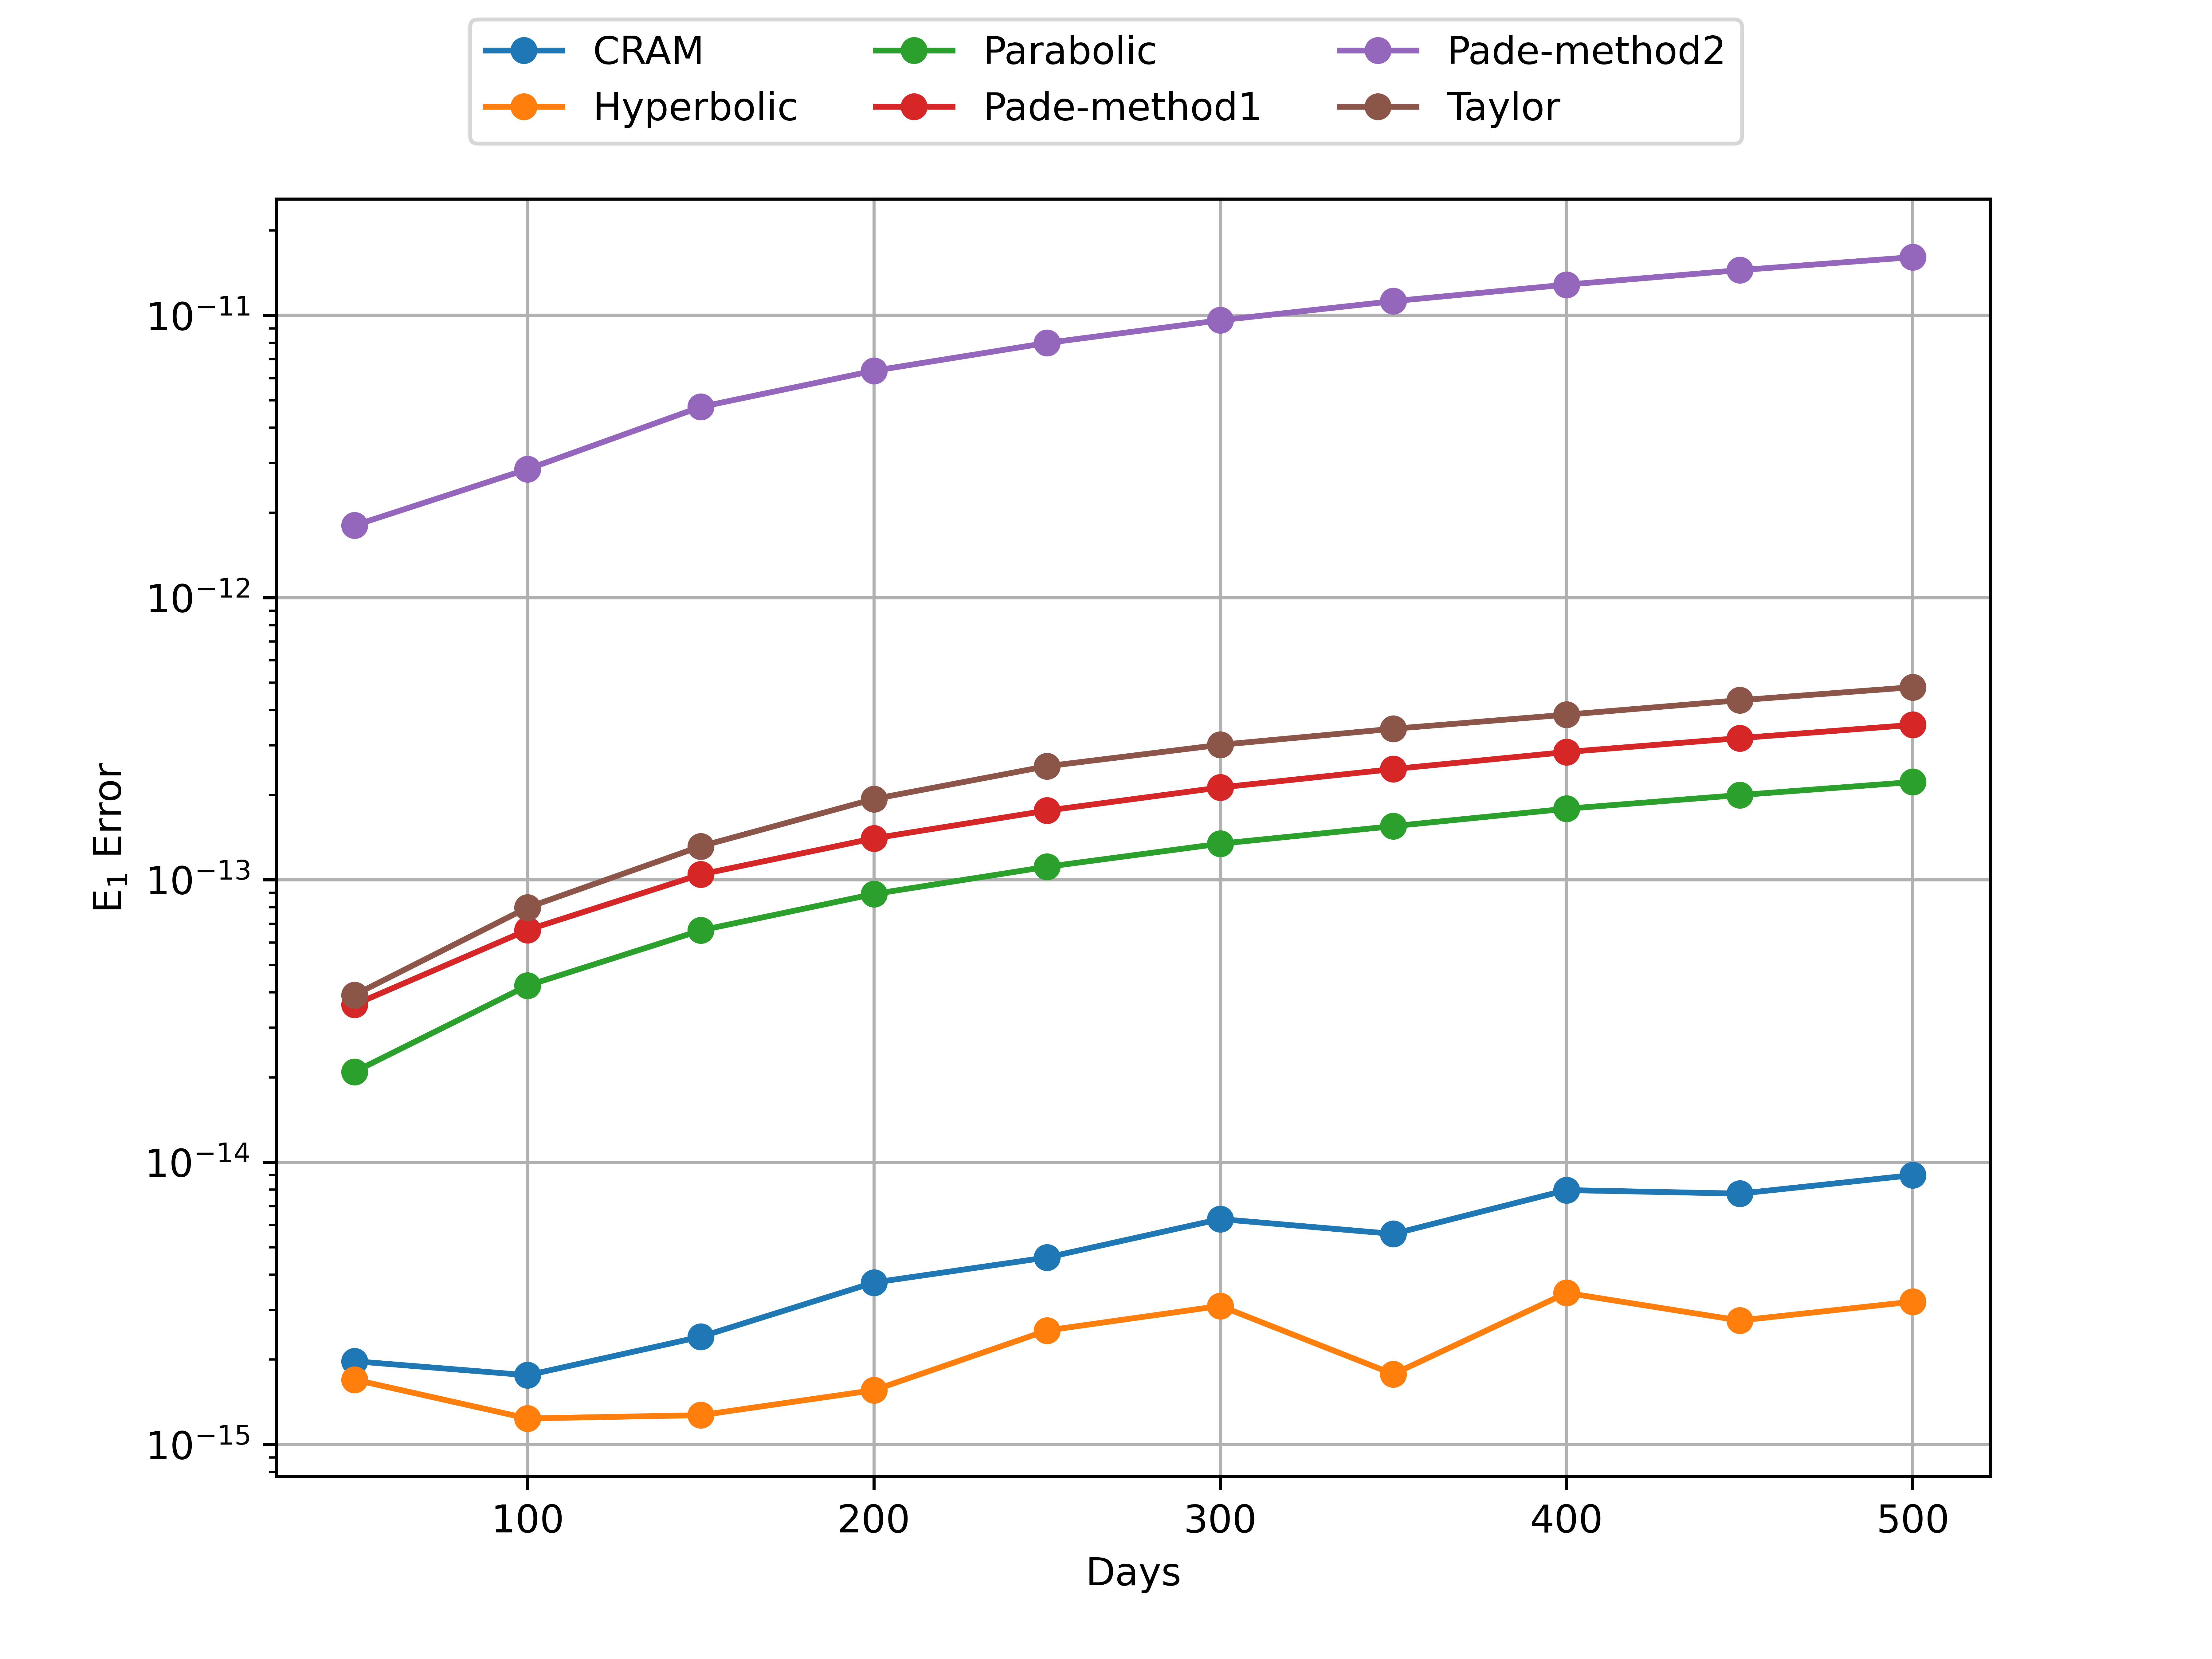
\includegraphics[width=6in]{images/chapter-5/progressionProblems/problem7/problem7E1ErrorerrorSteps4.png}
    \caption{Problem 7 E${}_{1}$ relative error with 4 sub-steps}
    \label{fig:problem7_E1_error_with_steps4}
\end{figure}

\clearpage

\begin{table}[p]
   \caption{\label{tab:problem7_run_times} Run Times for All Solvers in Depletion Case}
   \centering
   \begin{tabular}{ll}
   \hline
   Solver & Run time (sec)  \\
   \hline
   CRAM & 9.04e-03 \\
   Hyperbolic & 1.51e-02 \\
   Parabolic & 1.51e-02 \\
   Pad\'e-method 1 & 1.09e-03 \\
   Pad\'e-method 2 & 2.29e-03 \\
   Taylor & 5.76e-03 \\
   \hline
   \end{tabular}
\end{table}  

\clearpage

\begin{figure}[p]
    \centering
    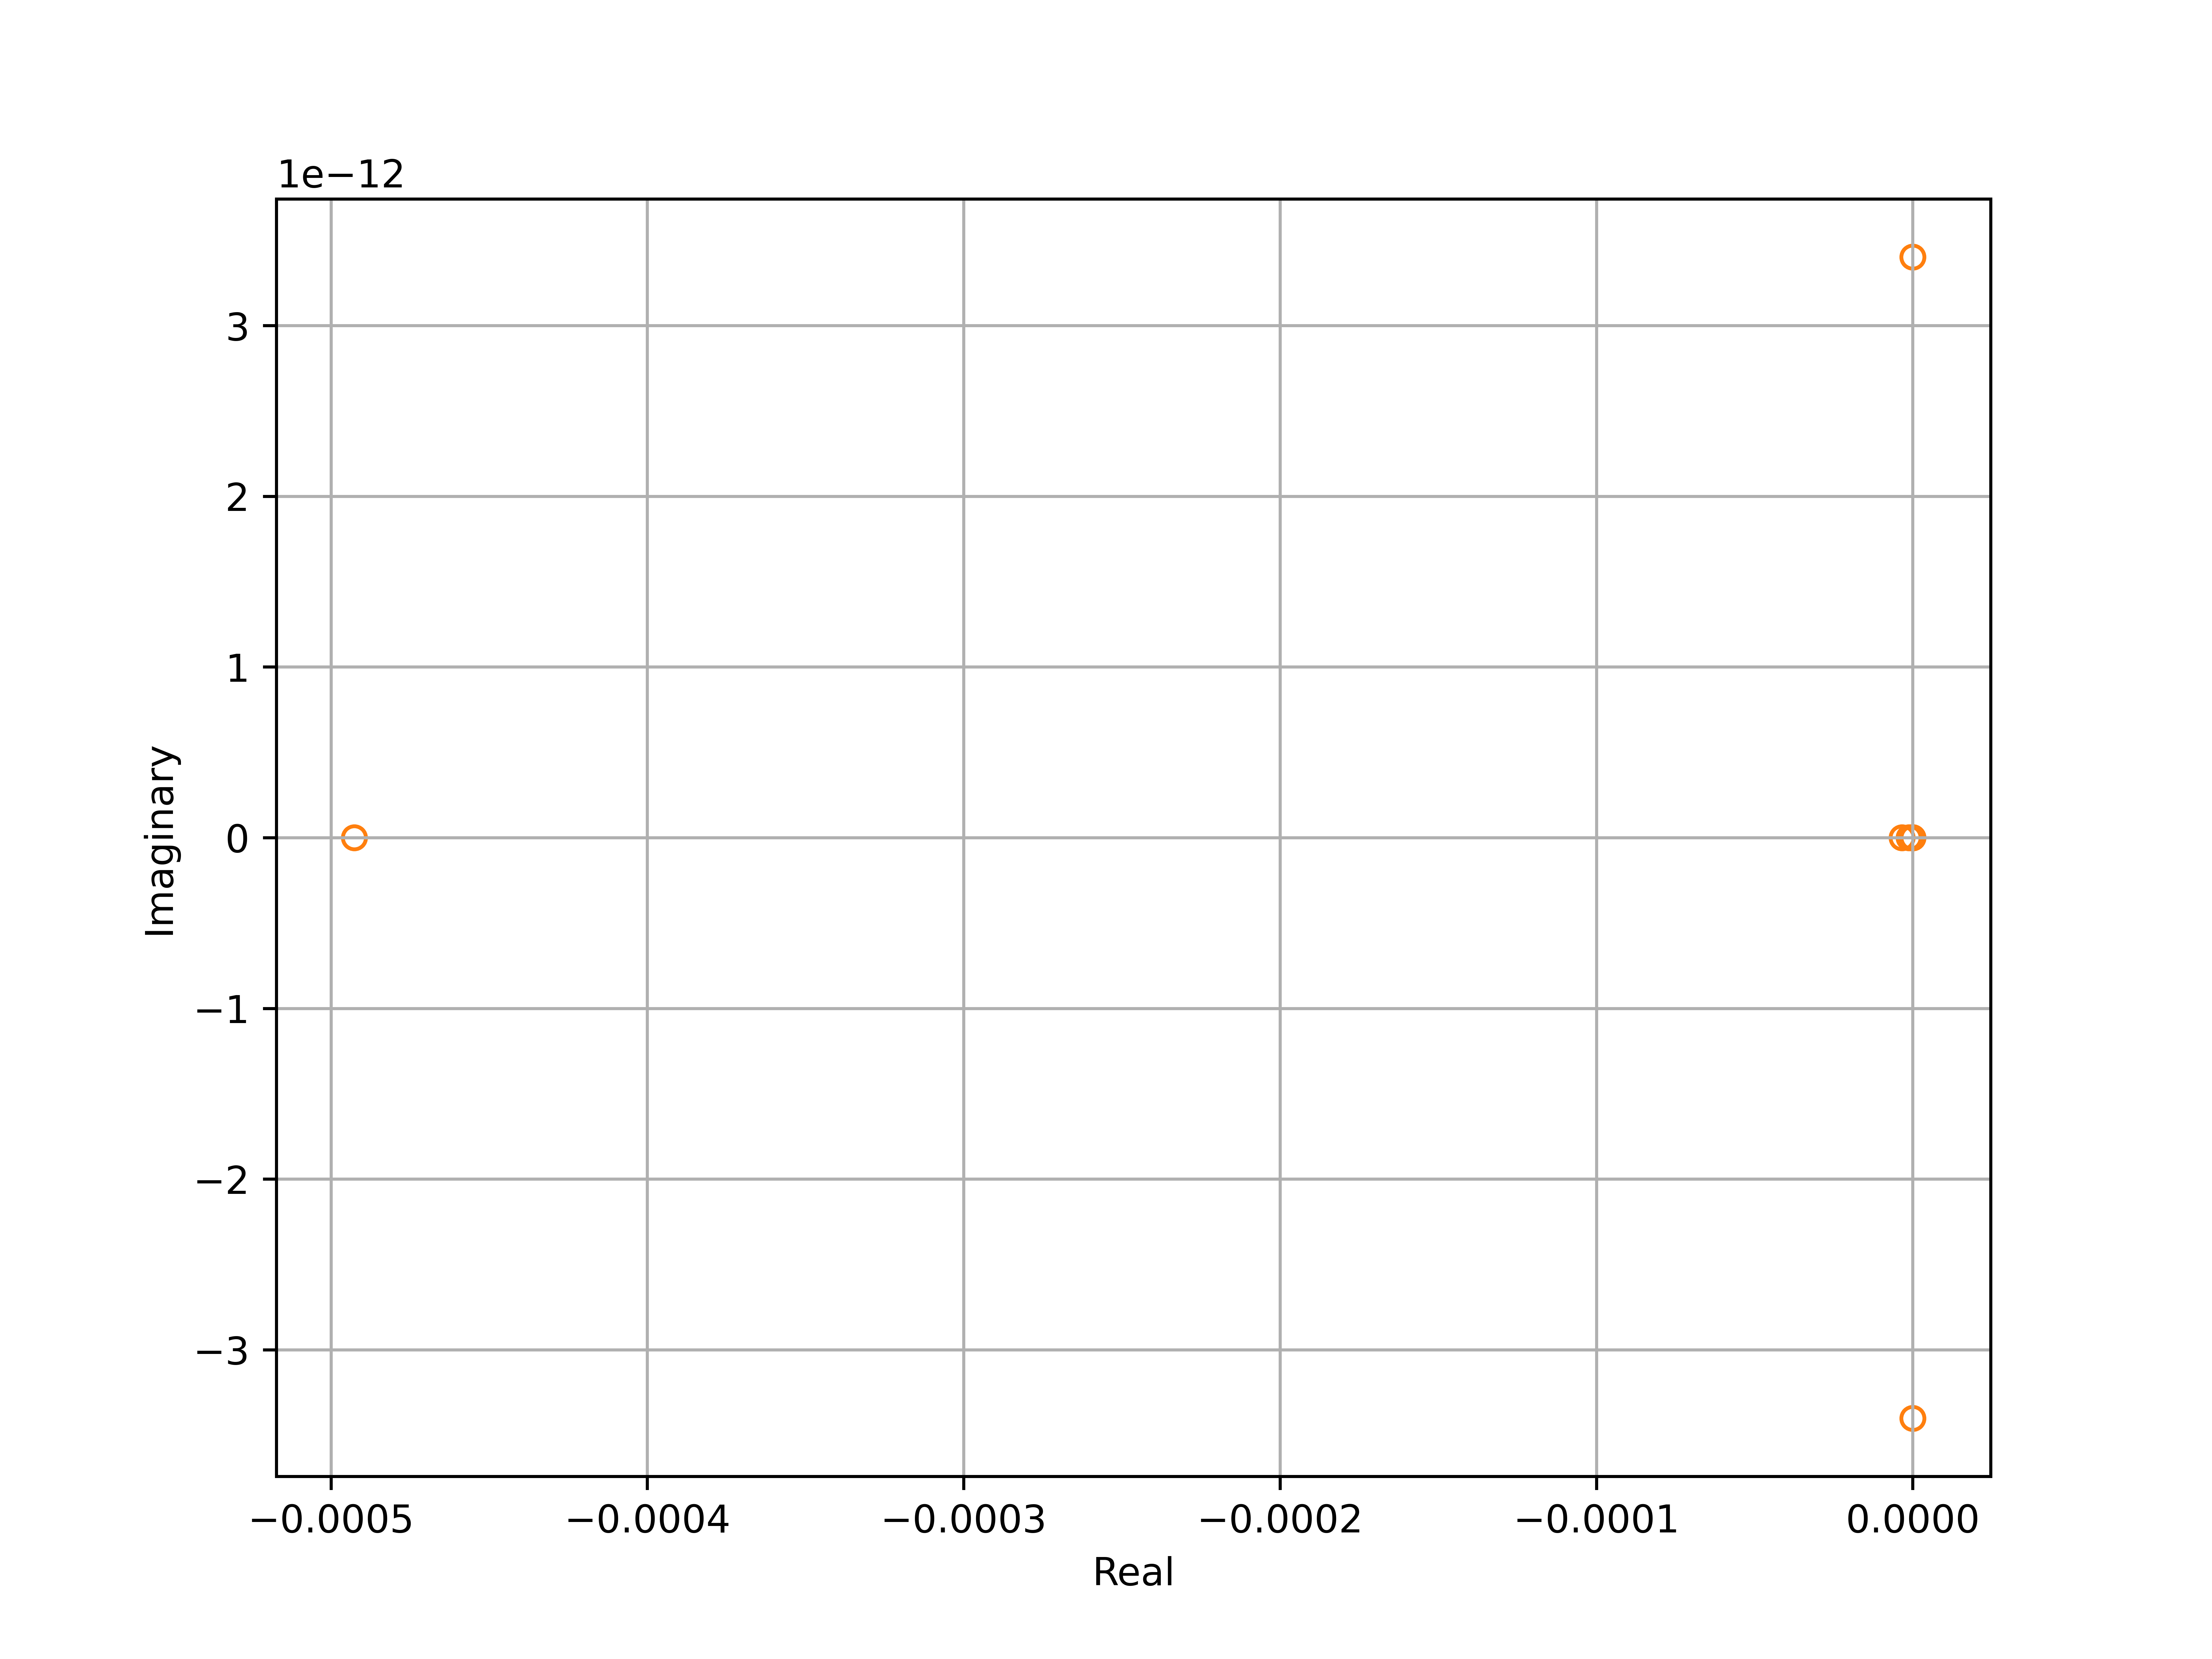
\includegraphics[width=6in]{images/chapter-5/progressionProblems/problem7/problem7Eigenvalues.png}
    \caption{Problem 7 eigenvalues}
    \label{fig:problem7_eigenvalues}
\end{figure}

\clearpage

\noindent placement of the eigenvalues, it is however, affected by the change is nuclide concentration over the time steps involved. Figure \ref{fig:problem7_nuclide_relative_error} shows the relative error of each nuclide at the 50 day time step for each of the Cauchy solvers. This Figure, along with Figure \ref{fig:problem7_solution} shows that the nuclides contributing to the highest two errors are the ones whos solution changes the most during that time step. 



\subsection{Problem 8}
This is an extension of problem 9 but for a fictitious "pipe" reactor which allows for the flow of isotopes due to a velocity. This is represented by:

\begin{equation}
\frac{d C_i}{dt} = -v\frac{\partial C_{i}}{\partial x} + \sum^9_{j = 1} A_{ij} C_j (x, t)
\end{equation}

\begin{equation}
i = \begin{dcases}
  1 , & \text{$^{233}$U}  \\
  2 , & \text{$^{234}$U}  \\
  3 , & \text{$^{235}$U}  \\
  4 , & \text{$^{236}$U}  \\
  5 , & \text{$^{237}$U}  \\
  6 , & \text{$^{238}$U}  \\
  7 , & \text{$^{239}$U}  \\
  8 , & \text{$^{239}$Pu} \\
  9 , & \text{$^{239}$Np} \\
\end{dcases}
\end{equation}

\noindent On the domain $x \in [0, 400]$, $t \in [0, 500]$. Subject to the periodic boundary conditions:

\begin{equation}
    C_{i}(0,t) = C_{i}(400,t).
\end{equation}

\clearpage

\begin{figure}[p]
    \centering
    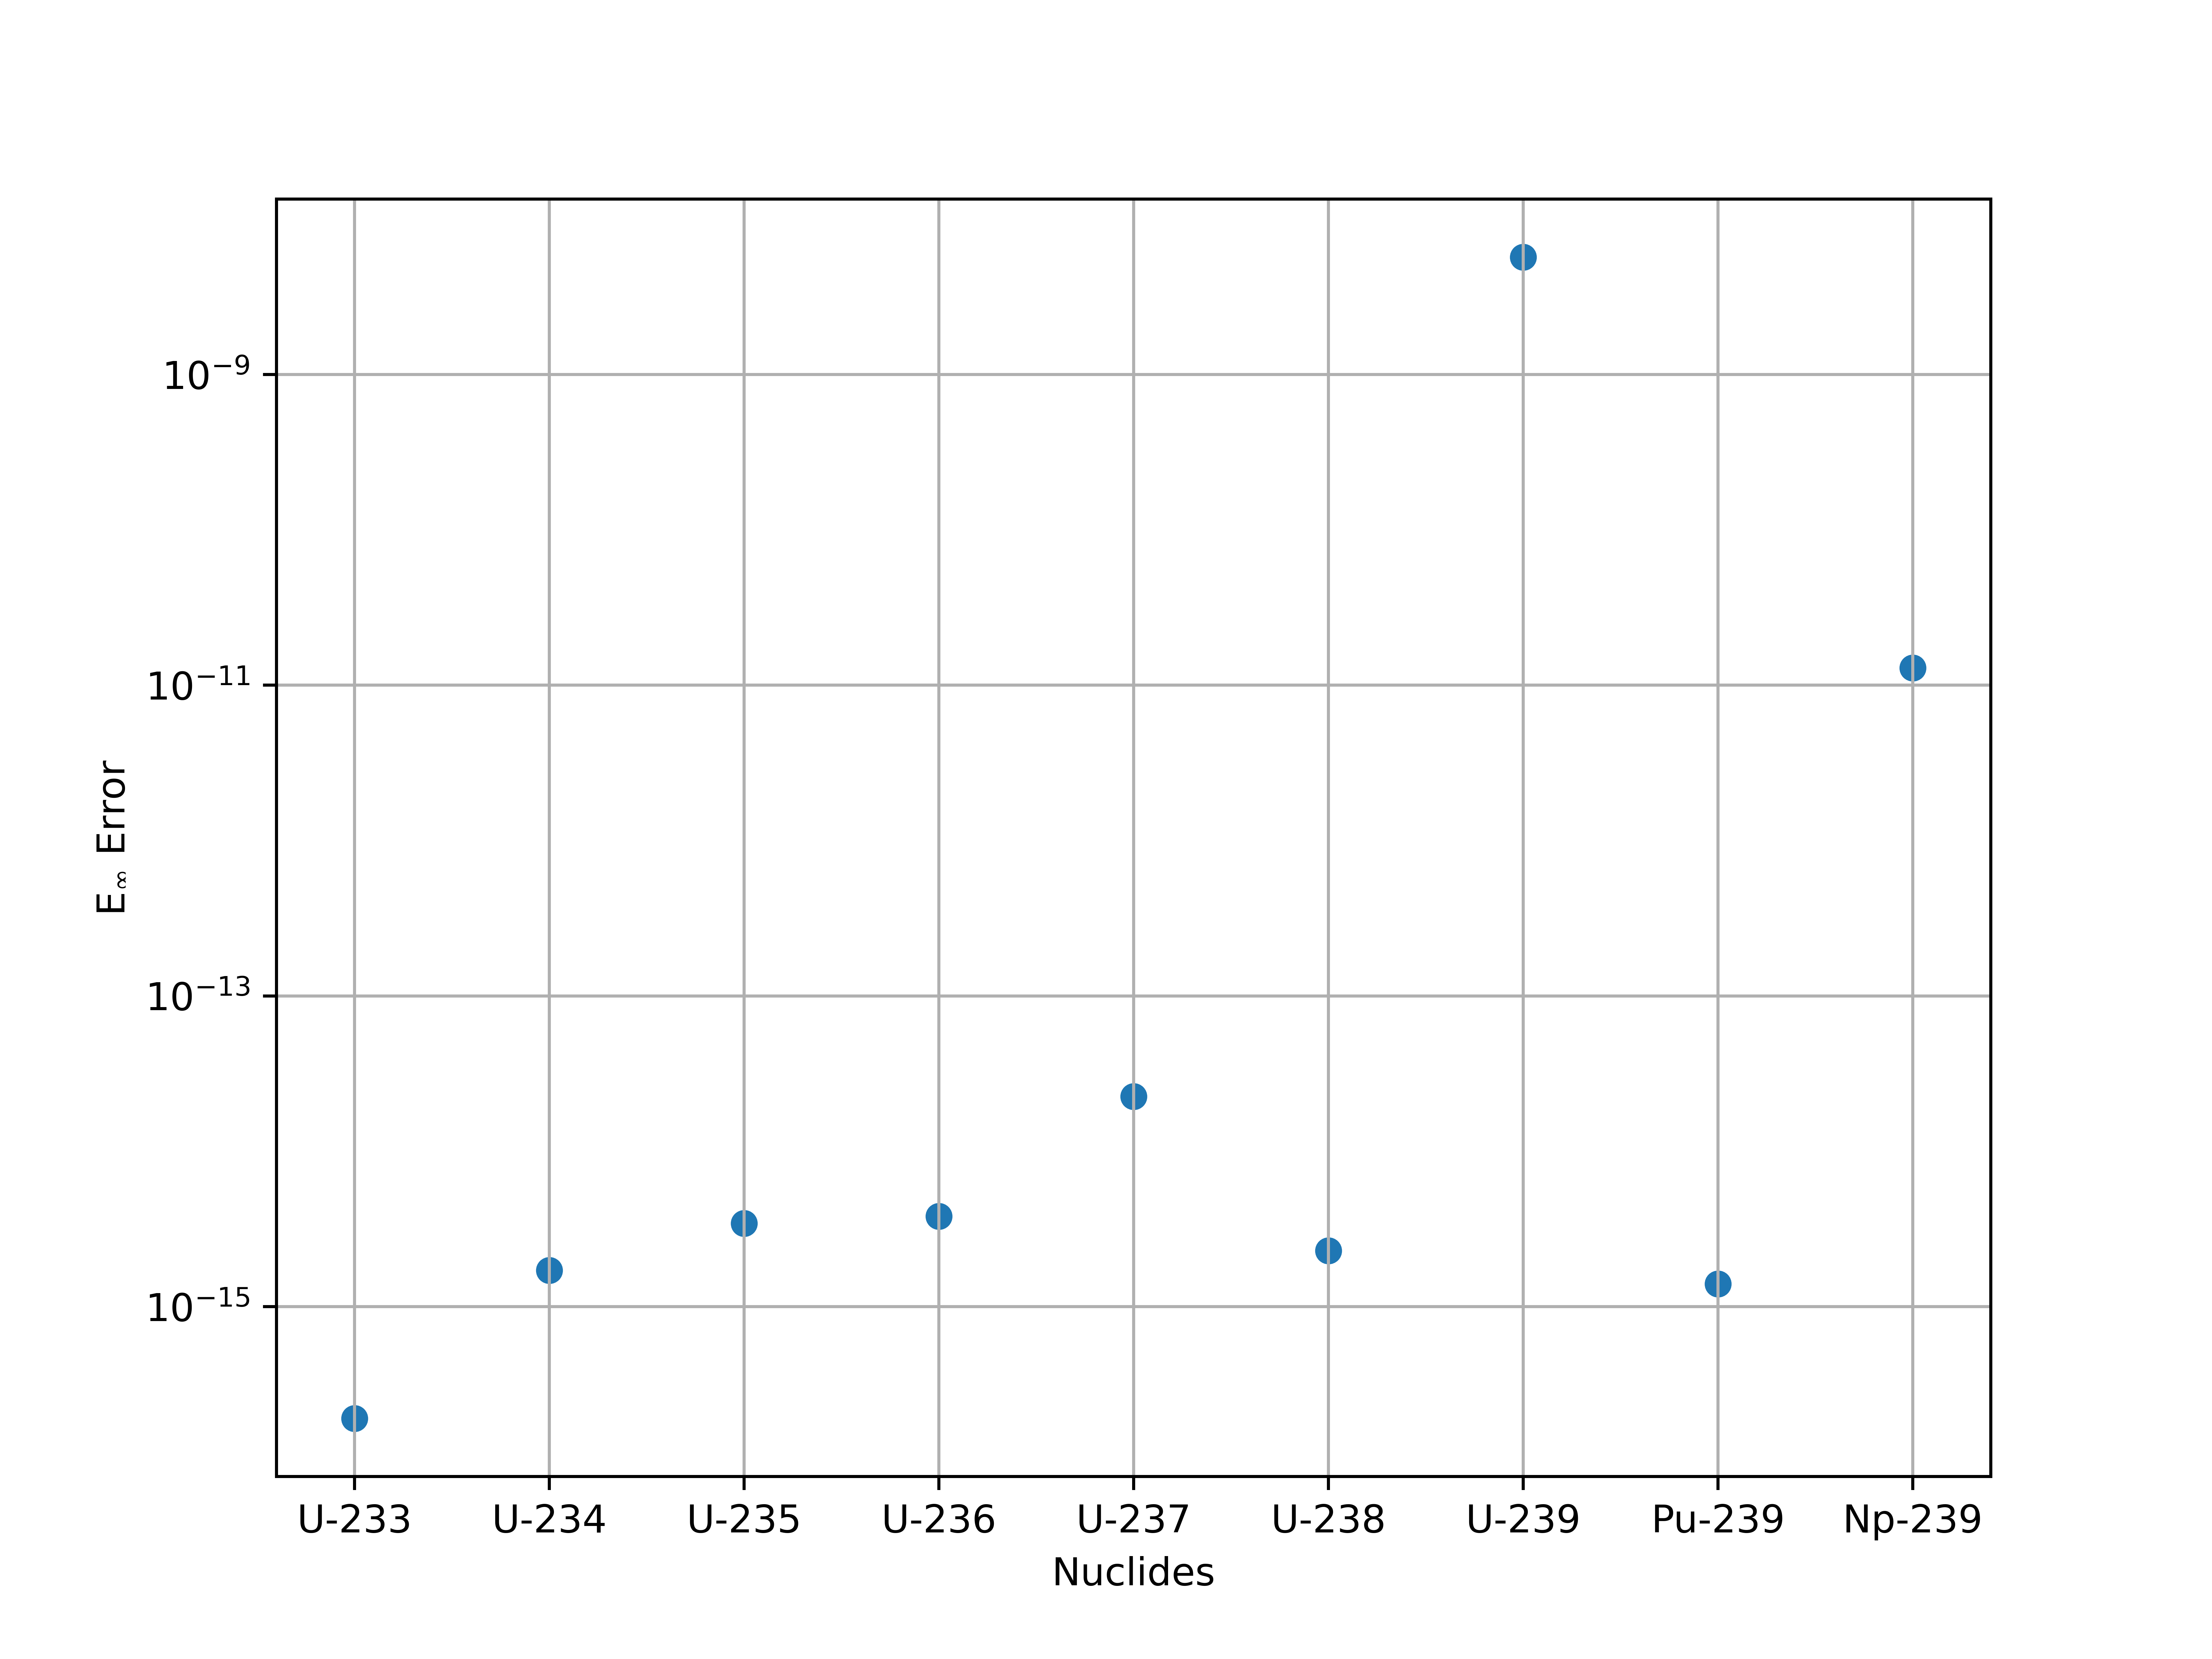
\includegraphics[width=6in]{images/chapter-5/progressionProblems/problem7/problem7NuclideErrorFirstStep.png}
    \caption{Problem 7 E${}_{\infty}$ relative error for each nuclide at the first time step}
    \label{fig:problem7_nuclide_relative_error}
\end{figure}

\clearpage

\noindent The neutron flux follows a sine function in the x-direction from $x \in [0, 200]$, half of the total length of the pipe. Four different velocities are chosen $ v = 2, 25, 50 $ and $100$, with a time step size of 50 days. This problem is ran with 3 different discretization sizes, with the number of cells varying from 10, 20 and 40. The higher order flux limiter functions are not used, with the first order upwind function being chosen for the convective flux. The reference solution is calculated using MATLAB. The eigenvalues for each velocity and discretization are shown in Figure \ref{fig:problem8_eigenvalues}, the left column are the eigenvalues of the transition matrix and the right column are the eigenvalues of the transition matrix multiplied by the time step size. As the number of cells increases the real and imaginary parts of the eigenvalues spread further out. This also happens as the velocity is increased. 



The E${}_{1}$ error for each velocity are shown for cells 10, 20 and 40 in Figures \ref{fig:problem8_E1_error_10cells}, \ref{fig:problem8_E1_error_20cells} and \ref{fig:problem8_E1_error_40cells}. Figure \ref{fig:problem8_E1_error_10cells} shows that all solvers but Pad\'e-method2 have around the same error. As the velocity is increased the error increases, with errors for velocities of 50 and 100 appear to be on top of one another except for Pad\'e-method2. Figure \ref{fig:problem8_E1_error_20cells} shows that for 20 cells, E${}_{1}$ errors for velocities 25, 50 and 100 fall on top of one another. Pad\'e-method1 again shows the worst error, with this error increasing as a function of velocity. Figure \ref{fig:problem8_E1_error_40cells} shows that the error for velocities 25 and 50 are about the same for all but Pad\'e-method2 and Taylor. Error for a velocity of 50 is only slightly higher than 25. Again Pad\'e-method2 shows the worst error, with the error increases with velocity. An important take away from these results is that each solver shows the same error behavior as a function of velocity. Indicating that the increased error seen in the Cauchy solvers do not result from the placement of the eigenvalues. Results for both the E${}_{\infty}$ and E${}_{2}$ errors for 10, 20 and 40 cells are shown in Appendix \ref{appen:results}, Figures \ref{fig:problem8_Einf_error_10cells}, \ref{fig:problem8_Einf_error_20cells}, \ref{fig:problem8_Einf_error_40cells}, \ref{fig:problem8_E2_error_10cells}, \ref{fig:problem8_E2_error_20cells} and \ref{fig:problem8_E2_error_40cells}. These error metrics show the same behavior as E${}_{1}$. 

Run times for each solver using 40 cells are shown for each velocity in Table \ref{tab:problem8_run_times}, each of the Cauchy solvers are shown with 2 sub-steps. None of the Cauchy solvers appear to show variation in run time with increased velocity but there is some slight differences with the Pad\'e solvers. The Taylor solver is most effected by the change in velocity and the reason is 

\clearpage

\begin{figure}[p]
    \centering
    \includegraphics[width=6in]{images/chapter-5/progressionProblems/problem8/problem8Eigenvalues.png}
    \caption{Problem 8 eigenvalues for each velocity and discretization}
    \label{fig:problem8_eigenvalues}
\end{figure}

\clearpage

\begin{figure}[p]
    \centering
    \includegraphics[width=6in]{images/chapter-5/progressionProblems/problem8/problem8E1ErrorWithVelocity10cells.png}
    \caption{Problem 8 E${}_{1}$ error with 10 cells}
    \label{fig:problem8_E1_error_10cells}
\end{figure}

\clearpage

\begin{figure}[p]
    \centering
    \includegraphics[width=6in]{images/chapter-5/progressionProblems/problem8/problem8E1ErrorWithVelocity20cells.png}
    \caption{Problem 8 E${}_{1}$ error with 20 cells}
    \label{fig:problem8_E1_error_20cells}
\end{figure}

\clearpage

\begin{figure}[p]
    \centering
    \includegraphics[width=6in]{images/chapter-5/progressionProblems/problem8/problem8E1ErrorWithVelocity40cells.png}
    \caption{Problem 8 E${}_{1}$ error with 40 cells}
    \label{fig:problem8_E1_error_40cells}
\end{figure}

\clearpage

\begin{table}[p]
   \caption{\label{tab:problem8_run_times} Run Times for All Solvers in Problem 8}
   \centering
   \begin{tabular}{lllll}
   \hline
    \multicolumn{1}{c}{} & \multicolumn{4}{c}{Run time (sec)}  \\
    Solver & Velocity 2 & Velocity 25 & Velocity 50 & Velocity 100 \\
   \hline
	CRAM & 7.16E-01 & 7.12E-01	& 7.14E-01 & 7.13E-01 \\
	Hyperbolic & 1.39E+00 & 1.38E+00	& 1.40E+00 & 1.38E+00 \\
	Parabolic & 1.40E+00 & 1.41E+00	& 1.40E+00 & 1.40E+00 \\
	Pad\'e-method1 & 1.70E+01 & 1.74E+01	& 1.91E+01 & 2.04E+01 \\
	Pad\'e-method2 & 2.42E+01 & 2.93E+01	& 2.76E+01 & 3.26E+01 \\
	Taylor & 3.93E+02 & 6.13E+03	& 1.27E+04 & 2.74E+04 \\
   \hline
   \end{tabular}
\end{table}  

\clearpage

\noindent found in the scaling and squaring method itself. For example, using the default parameters in the Taylor solver the required scaling parameter for velocities 2, 25, 50 and 100 are 486,179, 8,314,425, 18,132,096, and 39,544,424 for each time step. This causes a very large number of matrix vector multiplications. For the same velocities Pad\'e-method1 requires 19, 22, 23, 24 and Pad\'e-method2 requires 29, 35, 36, 38. While these run times for the Taylor solver can be mitigated by exploiting the computations from the previous time step, the time required to to compute a single time step is still quite large, about 1/10 of the total time required shown in Table \ref{tab:problem8_run_times}. The Krylov subspace method was applied to the Taylor solver, but using this method only increased the scaling and squaring value. For the Pad\'e solvers, the Krylov method is utilized in reducing the run time. These results are shown in Figure \ref{fig:problem8_E1_error_krylov} for the E$_{1}$ error and Figures \ref{fig:problem8_Einf_error_krylov} and \ref{fig:problem8_E2_error_krylov} for E$_{\infty}$ and E$_{2}$. The left most error point in these plots represents problem which is ran without using the Krylov subspace. Just by reducing the dimension by 9 increases the error a bit, followed by reaching a constant value for a number of Krylov dimensions. The error remains constant until increasing to a point where the solution blows up. These same trends occur for all 3 error metrics. 

\section{Case Studies}
The following are a selection of case studies which aim to explore libowskis' accuracy and performance with problems which come up in modeling MSRs. The small and large MSR cases require cross section data for the isotopes listed in Tables \ref{tab:small_nuclides} and \ref{tab:medium_nuclides}. This data is generated using ORIGEN f33 files with the Obiwan utility and exported to text files. These text file are then preprocessed by a python scrip (pyLibowski) to generate input files for libowski. For all of the case studies the first order upwind flux limiter function is used. For small and large lump and 2D transport studies, an MSRE type mesh is used. The description of this mesh and the calculation of other variables required for the model are in Appendix \ref{appen:nuclides}. For each of these studies there is no analytical solution. The reference solution is computed using the MATLAB method previously described. 

\clearpage

\begin{figure}[p]
    \centering
    \includegraphics[width=6in]{images/chapter-5/progressionProblems/problem8/problem8KrylovE1Error.png}
    \caption{Problem 8 E${}_{1}$ error for the Pad\'e solvers using the Krylov subspace with 40 cells}
    \label{fig:problem8_E1_error_krylov}
\end{figure}

\clearpage

For two of the case studies, classical numerical integration methods are shown. These two test are the neutron precursors and lump depletion. The purpose of showing results for these solvers is to demonstrate the why exponential time differencing is the preferred method for these problems.  

\subsection{Neutron precursors}
This problem examines a convection-driven flow with the 6 neutron precursor groups, as shown in Equations (\ref{eq:problem3}) and (\ref{eq:problem3flux}): 

\begin{equation}
\frac{\partial C_{i}}{\partial t} = -v_{x}\frac{\partial C_{i}}{\partial x} - v_{y}\frac{\partial C_{i}}{\partial y} + \beta_{i} \Psi (x, y) -\lambda_i C_{i},
\label{eq:problem3}
\end{equation}

\begin{equation}
\phi (x, y) = \begin{cases}
  \phi _0 \sin\left(\frac{\pi x}{50}\right)\sin\left(\frac{\pi y}{100}\right) , x \in [0,50], y \le 100 \\
  0\ , \text{otherwise},
  \label{eq:problem3flux}
\end{cases}
\end{equation}

\noindent where $i \in [1,6]$, $x \in [0, 50]$, $y \in [0, 400]$, $t \in [0, 60]$, $v_{x} = 0$, $\phi_0 = 1\text{E}13$ subject to the following boundary conditions:

\begin{equation}
    C_{i}(x,0) = C_{i}(x,400), \quad \frac{dC_{i}}{dx}(0,y) = 0, \quad \frac{dC_{i}}{dx}(50, y) = 0.
\end{equation}

\noindent This problem is ran at three different velocities, 25, 50 and 100. 

Coefficients for the system are shown in Table \ref{tab:precursorCoeffs} \cite{ott1985}. 
Each precursor had the same initial condition of zero, and the source term for each precursor was scaled in the x and y directions by the sine function. The spatial domain was modeled to mimic a core region extending from $y \in [0,100]$ and $x \in [0,50]$, with a core exterior loop modeled from $y \in [100, 400]$. 

The eigenvalues for this problem are shown in Figure \ref{fig:spectrum_neutron_precursors}. Each column represents the eigenvalues scaled by a single time step size and the CRAM, Hyperbolic and Parabolic solvers. Each row is a single solver with varying time step sizes. The contours represent the log base 10 absolute error of each scalar complex value on the real-imaginary plane. As the color becomes darker, the error becomes lower. While plotting there error contours along 

\clearpage

\begin{table}[p]
   \caption{\label{tab:precursorCoeffs} Parameters for Neutron Precursors}
   \centering
   \begin{tabular}{lll}
   \hline
   Group & $\lambda$ & $\beta$ \\
   \hline
   1 & 0.0127 & 0.0006 \\
   2 & 0.0317 & 0.00364 \\
   3 & 0.115 & 0.00349 \\
   4 & 0.311& 0.00628 \\
   5 & 1.4 & 0.00179\\
   6 & 3.87 & 0.0007 \\
   \hline
   \end{tabular}
\end{table} 

\clearpage

\begin{landscape}
\thispagestyle{mylandscape}
\begin{figure}[p]
    \centering
    \includegraphics[width=8in]{images/chapter-5/caseStudies/neutronPrecursors/neutronPrecursorsEigenvalues.png}
    \caption{Spectrum for the neutron precursors superimposed on the scalar complex error $\log_{10}|r(z)-e^{z}|$}
    \label{fig:spectrum_neutron_precursors}
\end{figure}
\end{landscape}

\clearpage

\noindent with the eigenvalues does not directly correlate to the total error for all matrices, examining these plots will provide insight into the accuracy of computing the matrix exponential with the Cauchy based methods. Just by examining the first column of Figure \ref{fig:spectrum_neutron_precursors}, it appears that based on the placement of the eigenvalues the accuracy of our solution should be very high for all three of the solvers. The eigenvalues for the lowest velocity are clusted in the center of the quadrature points. As the velocity is increased, the eigenvalues grow on the real axis at a larger rate than the imaginary axis. While the accuracy of the solution at 60 seconds is in fact while accuracy, shown in Figure \ref{fig:neutron_precursors_Einf_steps0}, at the first time step, the solution is quite inaccurate. This error can be drastically decreased in the first few time steps by applying the sub-stepping routine to each of these solvers, shown in Figure \ref{fig:neutron_precursors_Einf_dt1_with_substeps}. In Figure \ref{fig:neutron_precursors_Einf_dt1_with_substeps} each of the Cauchy solvers show dramatic decrease in error with the addition of sub-stepping. Other interesting behavior can be found by looking at the error as a function of time while using 12 substeps, shown in Figure \ref{fig:neutron_precursors_Einf_dt1_steps12}. When using zero sub-steps the error continues to decrease over the the time span. Using 12 sub-steps the error decreases to a point then gradually starts to increase. Both sub-stepping schemes end up leading to approximately the same solution at t = 60. The trend of the error beginning small and gradually increases can also be noticed in each of the Pad\'e solvers, with Pad\'e-method 2 being vastly more accuracy than Pad\'e-method 1. The Taylor solver also shows some decreased accuracy for the lower two velocities before self correcting and gradually increasing in error until t = 60. 

The second column in Figure \ref{fig:spectrum_neutron_precursors} shows the eigenvalues using a time step size of 10 seconds. Based on just the placement of the eigenvalues the error for a velocity of 100 should be the highest followed by 50 and 25. Figure \ref{fig:neutron_precursors_Einf_dt10_steps0} shows that for zero sub-steps confirms the behavior of error with velocity. At the first time step, the error is highest for a velocity of 100, followed by 50 and 25. What is interesting is the error at 60 seconds. The error for each of the solvers for a velocity of 100 is $~5\text{E}-9$. The initial error for velocity 50 is lower for the first time step, at t = 60, the error for a velocity of 100 is actually lower. The error for velocity 25 is lowest for the initial time step and for the final time step at t = 60. The Cauchy solvers also show the same error behavior with velocities 25 and 50. Hyperbolic 

\clearpage

\begin{figure}[p]
    \centering
    \includegraphics[width=5in]{images/chapter-5/caseStudies/neutronPrecursors/dt1/neutronPrecursorsEinfErrorerrorSteps0.png}
    \caption{Relative E$_{\infty}$ error with dt = 1 second for matrix exponential solvers in the neutron precursors case study using zero sub-steps for the Cauchy solvers}
    \label{fig:neutron_precursors_Einf_steps0}
\end{figure}

\clearpage

\begin{figure}[p]
    \centering
    \includegraphics[width=5in]{images/chapter-5/caseStudies/neutronPrecursors/dt1/neutronPrecursorsEinfErrorerrorWithSteps.png}
    \caption{Relative E$_{\infty}$ error for dt = 1 second as a function of sub-stepping in the neutron precursors case study for the first time step}
    \label{fig:neutron_precursors_Einf_dt1_with_substeps}
\end{figure}

\clearpage

\begin{figure}[p]
    \centering
    \includegraphics[width=5in]{images/chapter-5/caseStudies/neutronPrecursors/dt1/neutronPrecursorsEinfErrorerrorSteps12.png}
    \caption{Relative E$_{\infty}$ error with dt = 1 second for matrix exponential solvers in the neutron precursors case study using 12 sub-steps for the Cauchy solvers}
    \label{fig:neutron_precursors_Einf_dt1_steps12}
\end{figure}

\clearpage

\begin{figure}[p]
    \centering
    \includegraphics[width=5in]{images/chapter-5/caseStudies/neutronPrecursors/dt10/neutronPrecursorsEinfErrorerrorSteps0.png}
    \caption{Relative E$_{\infty}$ error with dt = 10 second for matrix exponential solvers in the neutron precursors case study using zero sub-steps for the Cauchy solvers}
    \label{fig:neutron_precursors_Einf_dt10_steps0}
\end{figure}

\clearpage

\noindent is the lowest error, followed by CRAM and Parabolic. Each of the series based solvers (Pad\'e and Taylor) show the same general trend with error that was seen in the dt = 1 runs. Pad\'e-method 1, showed the highest error of all solvers. Pad\'e-method 2, showed the second lowest error over all, with none of the zero sub-step Cauchy solvers acheiving lower accuracy. Tayler showed the lowest over all error. Figure \ref{fig:neutron_precursors_Einf_dt10_with_substeps} shows the error with sub-stepping for each of the Cauchy solvers. As with the dt = 1 results, there is dramatic accuracy imporvement with the first sub-step, about 10 orders of magnitude with 12 sub-steps. Each of the cauchy solvers begin with their errors spread out over many magnitudes but at 12 sub-steps the solvers are clustered around the same error magnitued. Results for each of the solvers with 12 sub-step Cauchy based algorithms are shown in Figure \ref{fig:neutron_precursors_Einf_dt10_steps12}. Each of the Cauchy solvers showed improvement for both in the first sub-step and the error at t = 60. This behavior was not seen for the dt = 1 runs, were regardless of the number of sub-steps, each of the Cauchy solvers showed about the same accuracy at t = 60. With 12 sub-steps, the hyperbolic solver becomes the lowest over all error, followed by CRAM, Taylor, Parabolic and Pad\'e-method 2. 

The last set of time step results are for exponential time differencing solvers that compute the final result with one time step (dt = 60) and for various explicit and implicit classical integrator schemes with different dt values. Looking back at the eigenvalues in Figure \ref{fig:spectrum_neutron_precursors}, all of the eigenvalues are pushed to a region which looks like their placement will not affect the error. Looking closer at the origin, the eigenvalues for velocity 25 and 50 are actually located in a region that might cause the solution accuracy to slightly degrade. Figure \ref{fig:neutron_precursors_Einf_dt60_with_substeps} shows errors for each of the Cauchy solvers with sub-stepping. For a velocity of 25, each of the solvers show improvment with each additional sub-step, where the error decays up to 12 sub-steps. What has not been seen before is the error behavior with velocities 50 and 100, where the error remains constant for a period then begins to decay. Error for a velocity of 100 also shows a step in which the error increases for a single sub-step for the CRAM and Parabolic solvers. The Hyperbolic solver does not show this behavior. Errors for each of the classical integrator solvers are shown in Figure \ref{fig:neutron_precursors_Einf_classical_integrator}. BDF 1 - 6 are implicit multi-step 

\begin{figure}[p]
    \centering
    \includegraphics[width=5in]{images/chapter-5/caseStudies/neutronPrecursors/dt10/neutronPrecursorsEinfErrorerrorWithSteps.png}
    \caption{Relative E$_{\infty}$ error for dt = 10 second as a function of sub-stepping in the neutron precursors case study for the first time step}
    \label{fig:neutron_precursors_Einf_dt10_with_substeps}
\end{figure}

\clearpage

\begin{figure}[p]
    \centering
    \includegraphics[width=5in]{images/chapter-5/caseStudies/neutronPrecursors/dt10/neutronPrecursorsEinfErrorerrorSteps12.png}
    \caption{Relative E$_{\infty}$ error with dt = 10 second for matrix exponential solvers in the neutron precursors case study using 12 sub-steps for the Cauchy solvers}
    \label{fig:neutron_precursors_Einf_dt10_steps12}
\end{figure}

\clearpage

\begin{figure}[p]
    \centering
    \includegraphics[width=5in]{images/chapter-5/caseStudies/neutronPrecursors/dt60/neutronPrecursorsEinfErrorerrorWithSteps.png}
    \caption{Relative E$_{\infty}$ error for dt = 60 second as a function of sub-stepping in the neutron precursors case study for the first time step}
    \label{fig:neutron_precursors_Einf_dt60_with_substeps}
\end{figure}

\clearpage

\begin{figure}[p]
    \centering
    \includegraphics[width=5in]{images/chapter-5/caseStudies/neutronPrecursors/dt60/neutronPrecursorsEinfErrorerrorIntegrators.png}
    \caption{Relative E$_{\infty}$ error for classical integrator solvers as a function of time step size at time = 60 seconds in neutron precursor case study}
    \label{fig:neutron_precursors_Einf_classical_integrator}
\end{figure}

\clearpage

\noindent backward differencing solvers of orders 1 - 6. Each of the other solvers belong to the family of explicit single-step Runge-Kutta methods. Solver errors are capped at 1E1, so solvers with error above this will be set to 1E1. For these results this indecates that solver was unstable at that time step size. From Figure \ref{fig:neutron_precursors_Einf_classical_integrator}, BDF1 and forward euler have the same errors for fine time step sizes but forward euler is unstable for large time step sizes. BDF1 is an implicit forward euler and it unconditionally stable. The midpoint and and BDF2 solvers also show the same trend as with forward euler and BDF1, because the midpoint solvers is a second order explicit mehtod. BDF3 and Kutta 3rd order show follow the same convergence rate at lower time step sizes with, Kutta 3rd order being slightly more accurate. As the order of the integrator increases past 3, the error behavior for finer time step sizes get slightly chaotic, going to a minmal value at dt = $10^{-2}$. The BDF6 solver also shows some instability for larger time step sizes. A summary of all solver errors at time = 60 seconds is shown in Figure \ref{fig:neutron_precursors_error_all_solvers}. All of the Cauchy solvers are shown with 12 sub-steps with dt = 60 and all of the classical integrator solvers are shown with the lowest errors for the given time step ranges. Taylor has the over all lowest error, followed by the 3rd and 4th order Kutta solvers. All solvers except for BDF1, forward euler and Pad\'e-method 1 have errors below $10^{-8}$.

Next the run times for each of the methods are discussed, the results for each method is taken as an average runtime of each of the velocities. Run times with the exponential time differencing solvers are shown in Figure \ref{fig:neutron_precursors_mat_exp_runtimes} for each time step size taken. Each of the Cauchy solvers in Figure \ref{fig:neutron_precursors_mat_exp_runtimes} is with zero sub-steps. The Pad\'e solvers take the longest, followed by the Hyperbolic and Parabolic solvers, CRAM and finally Taylor. For the largest time step size, the CRAM solver over takes the Taylor solver for the lowest run time. Run times for the classical integrator solvers are shown in Figure \ref{fig:neutron_precursors_classical_integrators_runtimes} as a function of time step size. Each of the BDF solvers start out with much different solve times, going from lowest order to highest following lowest run time to highest. As the time step size is decreased, they begin to converge to about the same run times. Each of the explicit Rung-Kutta solvers showed lower run times than their implicit counter parts. In general, the exponential time 

\clearpage

\begin{figure}[p]
    \centering
    \includegraphics[width=5in]{images/chapter-5/caseStudies/neutronPrecursors/dt60/neutronPrecursorsAllSolverErrors.png}
    \caption{Relative error for all solvers at time = 60 seconds in neutron precursor case study}
    \label{fig:neutron_precursors_error_all_solvers}
\end{figure}

\clearpage

\begin{figure}[p]
    \centering
    \includegraphics[width=5in]{images/chapter-5/caseStudies/neutronPrecursors/neutronPrecursorsMatExpRuntimes.png}
    \caption{Run times for the exponential time differencing solvers using zero sub-steps in neutron precursor case study}
    \label{fig:neutron_precursors_mat_exp_runtimes}
\end{figure}

\clearpage

\begin{figure}[p]
    \centering
    \includegraphics[width=5in]{images/chapter-5/caseStudies/neutronPrecursors/neutronPrecursorsIntegratorRuntimes.png}
    \caption{Run times for the classical integrators in neutron precursor case study}
    \label{fig:neutron_precursors_classical_integrators_runtimes}
\end{figure}

\clearpage

\noindent differencing solvers had higher run times for the same dt size however, the cost vs accuracy for the exponential time differencing solvers is better than the classical integrator methods. Run times as a function of sub-stepping for each of the Cauchy solvers is shown in Figure \ref{fig:neutron_precursors_substepping_cauchy_runtimes}. As expected, run times linearly increase as the number of sub-steps is increased, with the run times for Cauchy solvers with dt = 1 reaching values as high has 300 seconds. 

The Cauchy solvers were written to perform in parallel and performance study is conducted to assess this capability. Each solver is ran is such a way to evenly distribute the work load for each CPU core. A single 16th order CRAM solve consist of solving 8 independent linear systems, the 32nd order Hyperbolic and Parabolic solver each have 16 independent linear systems. In the case of CRAM, this leads to using 1, 2, 4 and 8 cores. For the Hyperbolic and Parabolic solvers, this set is extended to include 16 cores. Two sets of results are shown, the first is for speedup and the second is for parallel efficiency. Speedup is defined as run time for a single core over run time for multi-core. Parallel efficiency is the same ratio as speedup but also divided by the number of cores. Results for parallel speedup is shown in Figure \ref{fig:neutron_precursors_cauchy_speedup} and parallel efficiency in Figure \ref{fig:neutron_precursors_cauchy_parallel_eff}. Figure \ref{fig:neutron_precursors_cauchy_speedup} shows that for up to 8 cores, each of the solvers have close to the ideal linear speedup. As the number of cores grows larger to 16, the speedup diminishes some but overall the speedup is quite good. The Hyperbolic and Parabolic speedup closely resemble one another up to 8 cores, followed by the Parabolic solver showing slightly better speedup. Figure \ref{fig:neutron_precursors_cauchy_parallel_eff} shows a linear regression of parallel efficiency with all solvers, with CRAM diminishing more quickly. The differences in each of the Cauchy solvers might be within the complex valued coefficients causing some discrepancy in the linear solve time. 

\subsection{Lump depletion and mass transport}
This is a depletion problem using the selected isotopes in Table \ref{tab:small_nuclides} represented by the following equations:

\clearpage


\begin{figure}[p]
    \centering
    \includegraphics[width=5in]{images/chapter-5/caseStudies/neutronPrecursors/neutronPrecursorsCauchyRuntimes.png}
    \caption{Run times as a function of sub-stepping for Cauchy solvers in neutron precursor case study}
    \label{fig:neutron_precursors_substepping_cauchy_runtimes}
\end{figure}

\clearpage

\begin{landscape}
\thispagestyle{mylandscape}
\begin{figure}[p]
    \centering
    \includegraphics[width=8in]{images/chapter-5/caseStudies/neutronPrecursors/neutronPrecursorsCauchyParallelSpeedup.png}
    \caption{Parallel speedup for Cauchy solvers as various time step sizes and sub-steps in neutron precursor case study}
    \label{fig:neutron_precursors_cauchy_speedup}
\end{figure}
\end{landscape}

\clearpage

\begin{landscape}
\thispagestyle{mylandscape}
\begin{figure}[p]
    \centering
    \includegraphics[width=8in]{images/chapter-5/caseStudies/neutronPrecursors/neutronPrecursorsCauchyParallelEfficiency.png}
    \caption{Parallel efficiency for Cauchy solvers as various time step sizes and sub-steps in neutron precursor case study}
    \label{fig:neutron_precursors_cauchy_parallel_eff}
\end{figure}
\end{landscape}


\clearpage

\begin{equation}
\begin{split}
    \frac{\partial \rho_{i,l}}{\partial t}
    &=
    \sum_{j=1}^{N_{l}}\bigg[\frac{M_{i}}{M_{j}}\bigg(b_{j\rightarrow i}\lambda_{j} + 
    \sum_{k=1}^{K}\gamma_{j\rightarrow i,k}\sigma_{k,j}\phi \bigg)\rho_{j,l}
    - \bigg(\lambda_{i} + \phi\sum_{k=1}^{K} \sigma_{k,i}\bigg)\rho_{i, l} \bigg]\\ &+ \sum_{j=1}^{N_{w}} \bigg[-\frac{k_{w}A_{w}}{V}\rho_{i,l} \bigg] + \sum_{j=1}^{N_{g}} \bigg[  \frac{k_{g}A_{g}}{V}\bigg(\frac{1000H_{i}RT}{\alpha_{g}MM_{i}}\rho_{i, g} - \rho_{i,l}\bigg) \bigg],
    \label{eq:MSRLumpDepletionSmallLiquidPhase}
\end{split}
\end{equation}

\begin{equation}
\begin{split}
    \frac{\partial \rho_{i,w}}{\partial t} = \sum_{j=1}^{N_{w}}\bigg[&\frac{M_{i}}{M_{j}}\bigg(b_{j\rightarrow i}\lambda_{j} + 
    \sum_{k=1}^{K}\gamma_{j\rightarrow i,k}\sigma_{k,j}\phi \bigg)\rho_{j, w}
    - \bigg(\lambda_{i} + \phi\sum_{k=1}^{K} \sigma_{k,i}\bigg)\rho_{i, w} \bigg]\\ &+ \sum_{j=1}^{N_{w}} \bigg[\frac{k_{w}A_{w}}{V}\rho_{i,l} \bigg],
    \label{eq:MSRLumpDepletionSmallWallPhase}
\end{split}
\end{equation}

\begin{equation}
\begin{split}
    \frac{\partial \rho_{i,g}}{\partial t}
    =
    \sum_{j=1}^{N_{g}}\bigg[&\frac{M_{i}}{M_{j}}\bigg(b_{j\rightarrow i}\lambda_{j} + 
    \sum_{k=1}^{K}\gamma_{j\rightarrow i,k}\sigma_{k,j}\phi \bigg)\rho_{j, g}
    - \bigg(\lambda_{i} + \phi\sum_{k=1}^{K} \sigma_{k,i}\bigg)\rho_{i, \text{gas}} \bigg]\\ & + \sum_{j=1}^{N_{g}} \bigg[  \frac{k_{g}A_{g}}{V}\bigg(\rho_{i,l} - \frac{1000H_{i}RT}{\alpha_{g}MM_{i}}\rho_{i, g}\bigg) \bigg],
    \label{eq:MSRLumpDepletionSmallGasPhase}
\end{split}
\end{equation}

\noindent where $N_{l}$, $N_{w}$ and $N_{g}$ represent the set of species which exist in the liquid, wall and gas phases. A species that exist in the liquid, wall a gas phase is represented by $\rho_{i,l}$, $\rho_{i,w}$ and $\rho_{i,g}$.  This problem is ran with two different time ranges in mind. The first is computing the solution over 10 time steps in the range $t \in [0, 200]$, resulting in time step sizes of 20 days. The matrix exponential solvers are tested using this range. The second is by computing a single time step of just 20 days using the matrix exponential solvers and the classical integrator methods. This is done is such a way to understand the classical integrator requirements for solving for just one hypothetical depletion time step. 

\subsubsection{Small case}
Eigenvalues for this problem are shown in Figure \ref{fig:small_lumped_depletion_eigenvalues}. These eigenvalues are clustered around the negative real axis and will not have an affect on the error for Cauchy based solvers, even with a time step size of 20 days. Using zero sub-steps, results for all solvers are shown in Figure \ref{fig:small_lumped_depletion_Einf_steps0} over 200 days and in Figure \ref{fig:small_lumped_depletion_species_errors} for each isotope at t = 20 days. These errors shown the typical behavior that as been shown in other problems. The Cauchy based solvers begin with a large error which exponentially decreases as the solution progresses. Figure \ref{small_lumped_depletion_species_errors} shows very interesting results in that the error for the Cauchy solvers is driven by the error in actinide elements Pu, Am and Cm. For the CRAM and Hyperbolic solvers, every other element as error at or below $10^-{11}$. The Parabolic solver has all other elemental errors at or below $10^{-9}$. Pad\'e-method 2 has the highest error, with Pad\'e-method 1 and Taylor having approximately the same and over all lowest errors. The error for all three of these solvers begins low and gradually increases over the time span. 

Figure \ref{fig:small_lumped_depletion_Einf_with_substeps} shows Cauchy solvers errors as a function of sub-stepping. Each solver shows the same general trend of exponential decay in error with sub-stepping. The Parabolic solver has the highest error, with the CRAM and Hyperbolic solvers following closely in error. Figure \ref{fig:small_lumped_depletion_Einf_steps12} shows the error for each solver were each of the Cauchy solvers have 12 sub-steps. The Parabolic solver follows the same exponential decay trend as before. The CRAM and Hyperbolic solvers begin to decay until they reach a point where the error begins the climb. With sub-stepping, each of the Cauchy solvers achieves lower error at 200 days than the series solvers. 

Results for the classical integrator methods are shown in Figure \ref{fig:small_lumped_depletion_Einf_integrators}. These results are for a total time of 20 days, representing a single time step taken from the exponential time differencing solvers. Integrator errors are capped at 10, so any error which is 10 is unstable. All of the explicit solvers are unstable except for the lowest time step size. BDF1-3 show classical convergence rates for all time step sizes, BDF4-6 reach a minimal value before increasing with a reduction in time step size. This is the same behavior that was seen in the neutron precursors case study. 


\clearpage

\begin{figure}[p]
    \centering
    \includegraphics[width=5in]{images/chapter-5/caseStudies/smallLumpedDepletion/msrLumpedDepletionSmallEigenvalues.png}
    \caption{Eigenvalues for the small lumped depletion case}
    \label{fig:small_lumped_depletion_eigenvalues}
\end{figure}

\clearpage

\begin{figure}[p]
    \centering
    \includegraphics[width=5in]{images/chapter-5/caseStudies/smallLumpedDepletion/msrSmallLumpDepletionEinfErrorerrorSteps0.png}
    \caption{Relative E$_{\infty}$ error with dt = 20 days for matrix exponential solvers in the small lumped depletion case study using zero sub-steps for the Cauchy solvers}
    \label{fig:small_lumped_depletion_Einf_steps0}
\end{figure}

\clearpage

\begin{figure}[p]
    \centering
    \includegraphics[width=5in]{images/chapter-5/caseStudies/smallLumpedDepletion/msrLumpedDepletionSmallSteps0.png}
    \caption{Relative E$_{\infty}$ error for each isotope at t = 20 days for matrix exponential solvers in the small lumped depletion case study using zero sub-steps for the Cauchy solvers}
    \label{fig:small_lumped_depletion_species_errors}
\end{figure}

\clearpage

\begin{figure}[p]
    \centering
    \includegraphics[width=5in]{images/chapter-5/caseStudies/smallLumpedDepletion/msrSmallLumpedDepletionEinfErrorerrorWithSteps.png}
    \caption{Relative E$_{\infty}$ error for dt = 20 days as a function of sub-stepping in the small lumped depletion case study for the first time step}
    \label{fig:small_lumped_depletion_Einf_with_substeps}
\end{figure}

\clearpage

\begin{figure}[p]
    \centering
    \includegraphics[width=5in]{images/chapter-5/caseStudies/smallLumpedDepletion/msrSmallLumpDepletionEinfErrorerrorSteps12.png}
    \caption{Relative E$_{\infty}$ error with dt = 20 days for matrix exponential solvers in the small lumped depletion case study using 12 sub-steps for the Cauchy solvers}
    \label{fig:small_lumped_depletion_Einf_steps12}
\end{figure}

\clearpage

\begin{figure}[p]
    \centering
    \includegraphics[width=5in]{images/chapter-5/caseStudies/smallLumpedDepletion/msrSmallLumpedDepletionEinfErrorerrorIntegrators.png}
    \caption{Relative E$_{\infty}$ error with at time = 20 days for the classical integrator methods in small lumped depletion case}
    \label{fig:small_lumped_depletion_Einf_integrators}
\end{figure}

\clearpage


Run times for each of the Cauchy solvers as a function of sub-stepping are shown in Figure \ref{fig:small_lumped_depletion_Cauchy_runtimes}. The results show the typical linear run time increase with the number of sub-steps. Run times for the BDF integrators are shown in Figure \ref{fig:small_lumped_depletion_integrator_runtimes}. These shown the same trend shown in the neutron precursors case. As the largest time step size, each of the integrator run times are separated by order. These values are ranked from lowest to highest according to the BDF order. As the time step size is increased, each of the solvers converge to approximately the same value.  

A summary of results for each of the matrix exponential solvers and backward differencing solvers are shown in Table \ref{tab:small_lumped_depletion_runtimes} for both a single time step of 20 days and the total run time for 200 days with 10 20 day time steps for each of the matrix exponential solvers. Each of the Cauchy solvers is shown with 12 sub-steps. BDF solvers 4-6 reach their minimal error for time step sizes that are not the minimal value tested, resulting in smaller run times. CRAM, Hyperbolic, Pad\'e-method 1 and the Taylor solvers have the same order of magnitude for error. The Hyperbolic solver has twice the run time as CRAM and Taylor but takes about 14 times longer to run than CRAM. Pad\'e-method 1 is 42 times fast than CRAM. BDF3 also has the same order of magnitude as these solvers but takes 158 times longer than CRAM and 6,660 times longer than Pad\'e-method 1. BDF4 is an order of magnitude greater in accuracy but is 16 times slower than CRAM and 660 times slower than Pad\'e-method 1. BDF5 and 6 each have the lowest two errors with about double the run time as CRAM but show some unwanted behavior with low run times.  Each of the explicit solvers showed major instability and were not included in Table \ref{tab:small_lumped_depletion_runtimes}. 

Results for the parallel Cauchy solvers are shown in Figure \ref{fig:small_lumped_depletion_cauchy_speedup} for parallel speedup and Figure \ref{fig:small_lumped_depletion_cauchy_parallel_eff} for parallel efficiency. Figure \ref{fig:small_lumped_depletion_cauchy_speedup} shows that the parallel speed up increases as the number of sub-steps is increased. Figure \ref{fig:small_lumped_depletion_cauchy_parallel_eff} shows a linear decrease in parallel efficiency as the number of cores is increased. 


\clearpage

\begin{figure}[p]
    \centering
    \includegraphics[width=5in]{images/chapter-5/caseStudies/smallLumpedDepletion/msrLumpedDepletionSmallCauchyRuntimes.png}
    \caption{Run time as a function of sub-steps for Cauchy solvers in small lumped depletion case}
    \label{fig:small_lumped_depletion_Cauchy_runtimes}
\end{figure}

\clearpage

\begin{figure}[p]
    \centering
    \includegraphics[width=5in]{images/chapter-5/caseStudies/smallLumpedDepletion/msrLumpedDepletionSmallIntegratorRuntimes.png}
    \caption{Run time as a function of time step size for the BDF integrators in the small lumped depletion case}
    \label{fig:small_lumped_depletion_integrator_runtimes}
\end{figure}

\clearpage

\begin{table}[p]
\centering
\begin{threeparttable}
   \caption{\label{tab:small_lumped_depletion_runtimes} Summary of results for small lump depletion case}
   \begin{tabular}{lllll}
   \hline
   \multicolumn{1}{c}{} & \multicolumn{2}{c}{20 days\tnote{1}} & \multicolumn{2}{c}{200 days\tnote{2}} \\
   \cline{2-5} 
   Solver & Run time (sec) & E$_{\infty}$ error & Run time (sec) & E$_{\infty}$ error \\
   \hline
   CRAM\tnote{3} & 3.98E-01 & 3.78E-11 & 3.87E+00 & 2.66E-12 \\
   Hyperbolic\tnote{3} & 7.89E-01 & 2.49E-11 & 7.71E+00 & 2.68E-12 \\
   Parabolic\tnote{3} & 7.75E-01 & 1.34E-09 & 7.81E+00 & 1.31E-11 \\
   Pad\'e-method 1 & 9.43E-03 & 1.05E-11 & 9.48E-02 & 1.03E-10 \\
   Pad\'e-method 2 & 4.15E-02 & 4.74E-09 & 5.43E-01 & 4.01E-08 \\
   Taylor & 5.48E+00 & 1.30E-11 & 5.55E+01 & 1.13E-10 \\
   BDF1\tnote{4} & 7.28E+01 & 2.68E-04 & - & - \\
   BDF2\tnote{4} & 6.28E+01 & 1.06E-08 & - & - \\
   BDF3\tnote{4} & 6.29E+01 & 4.11E-11 & - & - \\
   BDF4\tnote{5} & 6.22E+00 & 4.51E-12 & - & - \\
   BDF5\tnote{6} & 6.55E-01 & 4.71E-12 & - & - \\
   BDF6\tnote{6} & 6.99E-01 & 6.68E-13 & - & - \\
   \hline
   \end{tabular}
	\begin{tablenotes}
      \small
      \item [1] Ran with one time step for the matrix exponential solvers
      \item [2] Ran with 10 time steps
      \item [3] Ran with 12 sub-steps
      \item [4] Results shown for dt = 17.28 seconds
      \item [5] Results shown for dt = 172.8 seconds
      \item [6] Results shown for dt = 1728 seconds
    \end{tablenotes}
\end{threeparttable}
\end{table} 

\clearpage

\begin{figure}[p]
    \centering
    \includegraphics[width=5in]{images/chapter-5/caseStudies/smallLumpedDepletion/msrLumpedDepletionSmallCauchyParallelSpeedup.png}
    \caption{Parallel speedup for Cauchy solvers as various time step sizes and sub-steps for the small lumped depletion case}
    \label{fig:small_lumped_depletion_cauchy_speedup}
\end{figure}

\clearpage

\begin{figure}[p]
    \centering
    \includegraphics[width=5in]{images/chapter-5/caseStudies/smallLumpedDepletion/msrLumpedDepletionSmallCauchyParallelEfficiency.png}
    \caption{Parallel efficiency for Cauchy solvers as various time step sizes and sub-steps for the small lumped depletion case}
    \label{fig:small_lumped_depletion_cauchy_parallel_eff}
\end{figure}

\clearpage


\subsubsection{Large case}
Eigenvalues for the large case are shown in Figure \ref{fig:large_lumped_depletion_eigenvalues}, these eigenvalues are clustered around the negative real axis and will not affect the accuracy of the Cauchy solvers. Results using zero sub-steps are shown in Figure \ref{fig:large_lumped_depletion_Einf_steps0}. These results are nearly identical to the small lumped depletion case except for the slightly elevated separation between the Taylor and Pad\'e-method 1 solvers. The Taylor solver has a slight increase in error between these two cases. Figure \ref{fig:large_lumped_depletion_Einf_with_substeps} also shows identical error behavior with increasing the number of sub-steps that was seen in the small case. The error exponential decays as a function of sub-steps. Figure \ref{fig:large_lumped_depletion_Einf_steps12} shows results for each solver were each of the Cauchy solver have 12 sub-steps. All solvers have the same behavior that was seen in the small case except for CRAM and the Hyperbolic solvers. The small case was able to achieve a lower minimal error than the large case. In both cases, the error decreases for the first few time steps but the large case increases in error to a greater degree as the solution progresses to 200 days. In this case, the CRAM and Hyperbolic solvers seem to more closely follow one another in error across the time span. Results for the classical integrator methods are shown in Figure \ref{fig:large_lumped_depletion_Einf_integrators} for a total time of 20 days. These errors are almost identical to the small case, showing that the added nuclides did not result in any notable change in error performance. 

Run times for each of the Cauchy solvers as a function of sub-stepping are shown in Figure \ref{fig:large_lumped_depletion_Cauchy_runtimes}. This trend is identical to the small case, only varying in run time. For the Hyperbolic and Parabolic solvers the run time for 12 sub-steps grow from about 8 seconds in the small case to a little over 20 seconds in the large case. CRAM increases from just under 8 seconds in the small case to about 12 seconds in the large case. Run time results for the classical integrator methods are shown in Figure \ref{fig:large_lumped_depletion_integrator_runtimes}. The same trend that was shown in the small case is seen here, except that the BDF1 integrator seems to converge closer to the other integrators as the time step size is decreased. 


Table \ref{tab:large_lumped_depletion_runtimes} shows a summary of results for the large lumped depletion case. These results show the same general behavior with the small case. CRAM, Hyperbolic, Taylor and BDF3 all have the same order of magnitude

\clearpage

\begin{figure}[p]
    \centering
    \includegraphics[width=5in]{images/chapter-5/caseStudies/largeLumpedDepletion/msrLumpedDepletionLargeEigenvalues.png}
    \caption{Eigenvalues for the large lumped depletion case}
    \label{fig:large_lumped_depletion_eigenvalues}
\end{figure}

\clearpage

\begin{figure}[p]
    \centering
    \includegraphics[width=5in]{images/chapter-5/caseStudies/largeLumpedDepletion/msrLargeLumpDepletionEinfErrorerrorSteps0.png}
    \caption{Relative E$_{\infty}$ error with dt = 20 days for matrix exponential solvers in the large lumped depletion case study using zero sub-steps for the Cauchy solvers}
    \label{fig:large_lumped_depletion_Einf_steps0}
\end{figure}

\clearpage

\begin{figure}[p]
    \centering
    \includegraphics[width=5in]{images/chapter-5/caseStudies/largeLumpedDepletion/msrLargeLumpedDepletionEinfErrorerrorWithSteps.png}
    \caption{Relative E$_{\infty}$ error for dt = 20 days as a function of sub-stepping in the large lumped depletion case study for the first time step}
    \label{fig:large_lumped_depletion_Einf_with_substeps}
\end{figure}

\clearpage

\begin{figure}[p]
    \centering
    \includegraphics[width=5in]{images/chapter-5/caseStudies/largeLumpedDepletion/msrlargeLumpDepletionEinfErrorerrorSteps12.png}
    \caption{Relative E$_{\infty}$ error with dt = 20 days for matrix exponential solvers in the large lumped depletion case study using 12 sub-steps for the Cauchy solvers}
    \label{fig:large_lumped_depletion_Einf_steps12}
\end{figure}

\clearpage

\begin{figure}[p]
    \centering
    \includegraphics[width=5in]{images/chapter-5/caseStudies/largeLumpedDepletion/msrLargeLumpedDepletionEinfErrorerrorIntegrators.png}
    \caption{Relative E$_{\infty}$ error with at time = 20 days for the classical integrator methods in large lumped depletion case}
    \label{fig:large_lumped_depletion_Einf_integrators}
\end{figure}

\clearpage

\begin{figure}[p]
    \centering
    \includegraphics[width=5in]{images/chapter-5/caseStudies/largeLumpedDepletion/msrLumpedDepletionLargeCauchyRuntimes.png}
    \caption{Run time as a function of sub-steps for Cauchy solvers in large lumped depletion case}
    \label{fig:large_lumped_depletion_Cauchy_runtimes}
\end{figure}

\clearpage


\begin{figure}[p]
    \centering
    \includegraphics[width=5in]{images/chapter-5/caseStudies/largeLumpedDepletion/msrLumpedDepletionLargeIntegratorRuntimes.png}
    \caption{Run time as a function of time step size for the BDF integrators in the large lumped depletion case}
    \label{fig:large_lumped_depletion_integrator_runtimes}
\end{figure}

\clearpage

\begin{table}[p]
\centering
\begin{threeparttable}
   \caption{\label{tab:large_lumped_depletion_runtimes} Summary of results for large lump depletion case}
   \begin{tabular}{lllll}
   \hline
   \multicolumn{1}{c}{} & \multicolumn{2}{c}{20 days\tnote{1}} & \multicolumn{2}{c}{200 days\tnote{2}} \\
   \cline{2-5} 
   Solver & Run time (sec) & E$_{\infty}$ error & Run time (sec) & E$_{\infty}$ error \\
   \hline
   CRAM\tnote{3} & 1.27E+00 & 3.78E-11 & 1.18E+01 & 5.83E-12 \\
   Hyperbolic\tnote{3} & 2.31E+00 & 2.49E-11 & 2.30E+01 & 5.88E-12 \\
   Parabolic\tnote{3} & 2.43E+00 & 1.34E-09 & 2.34E+01 & 1.31E-11 \\
   Pad\'e-method 1 & 2.82E-02 & 1.05E-11 & 2.97E-01 & 1.05E-10 \\
   Pad\'e-method 2 & 1.25E-01 & 4.74E-09 & 1.57E+00 & 4.01E-08 \\
   Taylor & 1.17E+01 & 1.50E-11 & 1.17E+02 & 1.49E-10 \\
   BDF1\tnote{4} & 1.40E+02 & 2.68E-04 & - & - \\
   BDF2\tnote{4} & 1.41E+02 & 1.06E-08 & - & - \\
   BDF3\tnote{4} & 1.40E+02 & 4.11E-11 & - & - \\
   BDF4\tnote{5} & 1.43E+01 & 4.51E-12 & - & - \\
   BDF5\tnote{6} & 1.55E+00 & 4.72E-12 & - & - \\
   BDF6\tnote{6} & 1.47E+00 & 9.51E-13 & - & - \\
   \hline
   \end{tabular}
	\begin{tablenotes}
      \small
      \item [1] Ran with one time step for the matrix exponential solvers
      \item [2] Ran with 10 time steps
      \item [3] Ran with 12 sub-steps
      \item [4] Results shown for dt = 17.28 seconds
      \item [5] Results shown for dt = 172.8 seconds
      \item [6] Results shown for dt = 1728 seconds
    \end{tablenotes}
\end{threeparttable}
\end{table} 

\clearpage

\noindent error with BEF4-6 having about an order of magnitude lower in error. Out of these solvers Pad\'e-method 1 had the lowest run time by 2 orders of magnitude. While the errors for the small and large cases are about the same, the run time almost doubles for each solver. 

Parallel results for the Cauchy solvers are shown in Figure \ref{fig:large_lumped_depletion_cauchy_speedup} for speedup and Figure \ref{fig:large_lumped_depletion_cauchy_parallel_eff}. Figure \ref{fig:large_lumped_depletion_cauchy_speedup} shows interesting results due to a lack in speedup from 1 core to zero cores. At 4 cores the speed up should be around 4 times but only has twice the speed up. This same trend is seen for the rest of the cores. Figure \ref{fig:large_lumped_depletion_cauchy_parallel_eff} mirrors there results with a sharp decrease in parallel efficiency at 2 cores, followed by a slow linear decrease. This behavior seems to be driven by the machine the case was ran on. 




\subsection{2D depletion and mass transport}
This is a depletion problem using the selected isotopes in Table \ref{tab:small_nuclides} represented by the following equations:

\begin{equation}
\begin{split}
    \frac{\partial \rho_{i,l}}{\partial t} + &v_{y}\frac{\partial \rho_{i,l}}{\partial x}
    = 
    \sum_{j=1}^{N_{l}}\bigg[\frac{M_{i}}{M_{j}}\bigg(b_{j\rightarrow i}\lambda_{j} + 
    \sum_{k=1}^{K}\gamma_{j\rightarrow i,k}\sigma_{k,j}\phi \bigg)\rho_{j, l}
   - \bigg(\lambda_{i} + \phi\sum_{k=1}^{K} \sigma_{k,i}\bigg)\rho_{i, l} \bigg]\\& + \sum_{j=1}^{N_{w}} \bigg[-\frac{k_{w}A_{w}}{V}\rho_{i,l} \bigg] + \sum_{j=1}^{N_{g}} \bigg[  \frac{k_{g}A_{g}}{V}\bigg(\frac{1000H_{i}RT}{\alpha_{g}MM_{i}}\rho_{i, g} - \rho_{i,l}\bigg) \bigg],
    \label{eq:MSR2DDepletionSmallLiquidPhase}
\end{split}
\end{equation}

\begin{equation}
\begin{split}
    \frac{\partial \rho_{i,w}}{\partial t} = \sum_{j=1}^{N_{w}}\bigg[&\frac{M_{i}}{M_{j}}\bigg(b_{j\rightarrow i}\lambda_{j} + 
    \sum_{k=1}^{K}\gamma_{j\rightarrow i,k}\sigma_{k,j}\phi \bigg)\rho_{j, w}
    - \bigg(\lambda_{i} + \phi\sum_{k=1}^{K} \sigma_{k,i}\bigg)\rho_{i, w} \bigg]\\ &+ \sum_{j=1}^{N_{w}} \bigg[\frac{k_{w}A_{w}}{V}\rho_{i,l} \bigg],
    \label{eq:MSR2DDepletionSmallWallPhase}
\end{split}
\end{equation}

\clearpage

\begin{figure}[p]
    \centering
    \includegraphics[width=5in]{images/chapter-5/caseStudies/largeLumpedDepletion/msrLumpedDepletionLargeCauchyParallelSpeedup.png}
    \caption{Parallel speedup for Cauchy solvers as various time step sizes and sub-steps for the large lumped depletion case}
    \label{fig:large_lumped_depletion_cauchy_speedup}
\end{figure}

\clearpage

\begin{figure}[p]
    \centering
    \includegraphics[width=5in]{images/chapter-5/caseStudies/largeLumpedDepletion/msrLumpedDepletionLargeCauchyParallelEfficiency.png}
    \caption{Parallel efficiency for Cauchy solvers as various time step sizes and sub-steps for the large lumped depletion case}
    \label{fig:large_lumped_depletion_cauchy_parallel_eff}
\end{figure}

\clearpage


\begin{equation}
\begin{split}
    \frac{\partial \rho_{i,g}}{\partial t} + v_{y}\frac{\partial \rho_{i,g}}{\partial x}
    =
    \sum_{j=1}^{N_{g}}\bigg[&\frac{M_{i}}{M_{j}}\bigg(b_{j\rightarrow i}\lambda_{j} + 
    \sum_{k=1}^{K}\gamma_{j\rightarrow i,k}\sigma_{k,j}\phi \bigg)\rho_{j, g}
    - \bigg(\lambda_{i} + \phi\sum_{k=1}^{K} \sigma_{k,i}\bigg)\rho_{i, g} \bigg]\\ & + \sum_{j=1}^{N_{g}} \bigg[  \frac{k_{g}A_{g}}{V}\bigg(\rho_{i,l} - \frac{1000H_{i}RT}{\alpha_{g}MM_{i}}\rho_{i, g}\bigg) \bigg],
    \label{eq:MSR2DDepletionSmallGasPhase}
\end{split}
\end{equation}

\noindent where $N_{l}$, $N_{w}$ and $N_{g}$ represent the set of species which exist in the liquid, wall and gas phases. A species that exist in the liquid, wall a gas phase is represented by $\rho_{i,l}$, $\rho_{i,w}$ and $\rho_{i,g}$.

\subsubsection{Small case}
Results for zero sub-steps for each of the matrix exponential solvers is shown in Figure \ref{fig:small_2D_depletion_Einf_steps0}. Each of the Cauchy solvers begin with large error which decrease to match the errors of Pad\'e-method 1 and Taylor. CRAM and Hyperbolic decrease faster than the Parabolic solver. Pad\'e-method 2 has the largest error at 200 days. Errors as a function of sub-stepping for each of the Cauchy solvers is shown in Figure \ref{fig:small_2D_depletion_Einf_with_substeps}. What is most interesting about these results compared to the lumped cases is that increases the sub-steps reduces the errors for CRAM and Hyperbolic until a point which it remains level. The Parabolic solver continues to decrease for all of the sub-steps. Errors for 12 sub-steps are shown in Figure \ref{fig:small_2D_depletion_Einf_steps12}. All of the solvers except for Pad\'e method 2 have approximately the same error. This is a trend that was not seen in the lumped depletion cases. Errors for the BDF solvers are shown in Figure \ref{fig:small_2D_depletion_Einf_integrators}. BDF1-3 show good convergence rates over the time span. BEF4-6 show good convergence for the first three time steps, then the errors remain constant for the last two time steps. 

Run times as a function of sub-stepping for the Cauchy solvers is shown in Figure \ref{fig:small_2D_depletion_Cauchy_runtimes}. These results show the typical linear run time increase for each solver. The Hyperbolic solver shows slightly higher run time than the parabolic solver. Run times for the BDF solvers is 

\clearpage

\begin{figure}[p]
    \centering
    \includegraphics[width=5in]{images/chapter-5/caseStudies/small2DDepletion/msrSmall2DDepletionEinfErrorerrorSteps0.png}
    \caption{Relative E$_{\infty}$ error with dt = 20 days for matrix exponential solvers in the small 2D depletion case study using zero sub-steps for the Cauchy solvers}
    \label{fig:small_2D_depletion_Einf_steps0}
\end{figure}

\clearpage

\begin{figure}[p]
    \centering
    \includegraphics[width=5in]{images/chapter-5/caseStudies/small2DDepletion/msrSmall2DDepletionEinfErrorerrorWithSteps.png}
    \caption{Relative E$_{\infty}$ error for dt = 20 days as a function of sub-stepping in the small 2D depletion case study for the first time step}
    \label{fig:small_2D_depletion_Einf_with_substeps}
\end{figure}

\clearpage

\begin{figure}[p]
    \centering
    \includegraphics[width=5in]{images/chapter-5/caseStudies/small2DDepletion/msrSmall2DDepletionEinfErrorerrorSteps12.png}
    \caption{Relative E$_{\infty}$ error with dt = 20 days for matrix exponential solvers in the small 2D depletion case study using 12 sub-steps for the Cauchy solvers}
    \label{fig:small_2D_depletion_Einf_steps12}
\end{figure}

\clearpage

\begin{figure}[p]
    \centering
    \includegraphics[width=5in]{images/chapter-5/caseStudies/small2DDepletion/msrSmall2DDepletionEinfErrorerrorIntegrators.png}
    \caption{Relative E$_{\infty}$ error with at time = 20 days for the classical integrator methods in small 2D depletion case}
    \label{fig:small_2D_depletion_Einf_integrators}
\end{figure}

\clearpage

\begin{figure}[p]
    \centering
    \includegraphics[width=5in]{images/chapter-5/caseStudies/small2DDepletion/msr2DDepletionSmallCauchyRuntimes.png}
    \caption{Run time as a function of sub-steps for Cauchy solvers in small 2D depletion case}
    \label{fig:small_2D_depletion_Cauchy_runtimes}
\end{figure}

\clearpage

\noindent shown in Figure \ref{fig:small_2D_depletion_integrator_runtimes}, showing the typical behavior of each of the solvers being spread out for large time step sizes. These values converge as the time step size grows smaller. 

A summary of results for each of solvers tested is shown in Table \ref{tab:small_2D_depletion_runtimes}. While the values for the lowest errors are shown, it should be noted that BEF4-6 had only slightly better accuracy than the previous time step. At the previous time step BEF4-6 has run times of 712, 768 and 792 seconds, each of which is still greater than each of the matrix exponential solver but Taylor. CRAM, Hyperbolic, Pad\'e-method 1, Taylor and 3 of the BDF solvers all have about the same error. Taylor takes the longest by one to two orders of magnitude for the matrix exponential solvers. 

Results for the parallel Cauchy solvers are shown in Figures \ref{fig:small_2D_depletion_cauchy_speedup} and \ref{fig:small_2D_depletion_cauchy_parallel_eff}. These results show good parallel speed up for each of the sub-steps, reaching 12 times the speed up for 16 cores in the Hyperbolic and Parabolic solvers. The parallel efficiency shows an apparent elevated value for 2 processors when using 6 and 12 sub-steps. This is due to the slight differences in run times each time the problem is ran. After two cores the parallel efficiency shows the common linear decrease as the number of cores is increased. 

\subsubsection{Large case}


\clearpage

\begin{figure}[p]
    \centering
    \includegraphics[width=5in]{images/chapter-5/caseStudies/small2DDepletion/msr2DDepletionSmallIntegratorRuntimes.png}
    \caption{Run time as a function of time step size for the BDF integrators in the small 2D depletion case}
    \label{fig:small_2D_depletion_integrator_runtimes}
\end{figure}

\clearpage

\begin{table}[p]
\centering
\begin{threeparttable}
   \caption{\label{tab:small_2D_depletion_runtimes} Summary of results for small 2D depletion case}
   \begin{tabular}{lllll}
   \hline
   \multicolumn{1}{c}{} & \multicolumn{2}{c}{20 days\tnote{1}} & \multicolumn{2}{c}{200 days\tnote{2}} \\
   \cline{2-5} 
   Solver & Run time (sec) & E$_{\infty}$ error & Run time (sec) & E$_{\infty}$ error \\
   \hline
   CRAM\tnote{3} & 2.47E+02 & 9.60E-10 & 2.46E+03 & 8.67E-09 \\
   Hyperbolic\tnote{3} & 4.65E+02 & 9.60E-10 & 4.54E+03 & 8.67E-09 \\
   Parabolic\tnote{3} & 4.63E+02 & 1.24E-08 & 4.42E+03 & 8.67E-09 \\
   Pad\'e-method 1 & 9.12E+01 & 9.78E-10 & 8.97E+02 & 8.84E-09 \\
   Pad\'e-method 2 & 1.88E+02 & 5.93E-08 & 1.87E+03 & 5.92E-07 \\
   Taylor & 5.16E+03 & 9.48E-10 & 5.18E+04 & 8.40E-09 \\
   BDF1\tnote{4} & 6.17E+03 & 2.68E-03 & - & - \\
   BDF2\tnote{4} & 6.28E+03 & 1.06E-06 & - & - \\
   BDF3\tnote{4} & 6.36E+03 & 9.39E-10 & - & - \\
   BDF4\tnote{4} & 6.12E+03 & 9.39E-10 & - & - \\
   BDF5\tnote{4} & 6.83E+03 & 9.99E-10 & - & - \\
   BDF6\tnote{4} & 6.45E+03 & 9.43E-10 & - & - \\
   \hline
   \end{tabular}
	\begin{tablenotes}
      \small
      \item [1] Ran with one time step for the matrix exponential solvers
      \item [2] Ran with 10 time steps
      \item [3] Ran with 6 sub-steps
      \item [4] Results shown for dt = 172.8 seconds
    \end{tablenotes}
\end{threeparttable}
\end{table} 

\begin{figure}[p]
    \centering
    \includegraphics[width=5in]{images/chapter-5/caseStudies/small2DDepletion/msrSmall2DDepletionCauchyParallelSpeedup.png}
    \caption{Parallel speedup for Cauchy solvers as various time step sizes and sub-steps for the large lumped depletion case}
    \label{fig:small_2D_depletion_cauchy_speedup}
\end{figure}

\clearpage

\begin{figure}[p]
    \centering
    \includegraphics[width=5in]{images/chapter-5/caseStudies/small2DDepletion/msrSmall2DDepletionCauchyParallelEfficiency.png}
    \caption{Parallel efficiency for Cauchy solvers as various time step sizes and sub-steps for the small 2D depletion case}
    \label{fig:small_2D_depletion_cauchy_parallel_eff}
\end{figure}

\clearpage
